\documentclass[
%pdftex,
paper=a4,
11pt,
%BCOR=15mm,
%DIV=10,
twoside,
open=right,
parskip=half-,
headinclude=true,
headsepline,
%footsepline,
titlepage=true,
%chapterprefix=on,
%appendixprefix=on,
headings=normal,
bibliography=totoc,
listof=totoc,
listof=nochaptergap,
%leqno,
%fleqn,
%draft=true,
numbers=noenddot,
ngerman
]{scrbook}
%\evensidemargin0mm
%\oddsidemargin15mm

\usepackage{hyphsubst}
\HyphSubstIfExists{ngerman-x-latest}{%
	\HyphSubstLet{ngerman}{ngerman-x-latest}}{}
\usepackage[ngerman]{babel}
\usepackage[T1]{fontenc}
\usepackage[utf8]{inputenc}
\usepackage{textcomp}
\usepackage{lmodern}
\usepackage{times}
\fontfamily{ptm}\selectfont
\KOMAoptions{DIV=last}
\usepackage[final,babel]{microtype}

\setkomafont{disposition}{\normalcolor\bfseries}

\usepackage{chngcntr}
\counterwithout{figure}{chapter}
\counterwithout{table}{chapter}

\usepackage{etoolbox}
\usepackage{tabularx}
\usepackage{tabulary}
\usepackage{colortbl}
\usepackage{subcaption}
\captionsetup[subfigure]{list=true, font=small, labelfont=bf, 
	labelformat=brace, position=top}
\usepackage{multirow}
\usepackage{enumitem}
\newlist{titemize}{itemize}{1}																% neue Listenumgebung für Tabellen 
\setlist[titemize]{nosep, label=\textbullet, after=\strut, align=left, leftmargin=*}

\DeclareMicrotypeSet*[tracking]{my}%
  { font = */*/*/sc/* }%
\SetTracking{ encoding = *, shape = sc }{ 45 }


\usepackage[inner=34mm, outer=30mm]{geometry}
\usepackage[automark]{scrlayer-scrpage}
\pagestyle{scrheadings}																		% lebendiger Seitentitel

\raggedbottom
\setlength{\parindent}{0em}
\setlength{\parskip}{1ex}

\newcommand{\mydate}{\today}

\usepackage{amsmath}																		% erweiterter Mathematiksatz
\usepackage{amssymb}																		% weitere Mathematiksymbole
\renewcommand\theequation{\thechapter-\arabic{equation}}

\usepackage{pdflscape} 
\usepackage[tight,nice]{units}																% ermöglicht Angabe physikal. Größen
\usepackage[version-1-compatibility]{siunitx}
\sisetup{detect-family, locale=DE}
\usepackage{booktabs}

\usepackage{dcolumn}																		% für gezielte Ausrichtung von Zahlen in Tabellen

\usepackage{url}																			% für url-Angaben

\usepackage{float}
\usepackage{wasysym}

\usepackage{relsize}																		% Schriftgrüßen nicht absolut, sondern relativ angeben
\usepackage{setspace}																		% Zeilenabstand

\usepackage[margin=10pt,font=small,labelfont=bf,labelsep=endash,format=hang,figurename={Abb.}, tablename={Tab.}
]{caption}																					% für schönere Unterschriften bei Abbildungen und Tabellen

\usepackage{calc}
%\usepackage[printonlyused]{acronym}

\usepackage[section]{placeins}																% Einfügen einer "FloatBarrier"

\usepackage[final]{graphicx}																% Paket zum Einbinden von Bildern, Option "final" hebt die globale "draft" bei Abbildungen auf

\usepackage{textpos}																		% für millimetergenaue Paltzierung von Text(Grafik-)blöcken
\usepackage[update]{epstopdf}

\usepackage{lipsum}																			% Paket für "Lorem Ipsum" Paragraphen
\usepackage{pdfpages}
\usepackage[]{todonotes}
%\usepackage{pdfcomment}

\usepackage{scrhack}																		% Damit keine Warnung \float@addtolists auftritt (bei verwendung von listings)
\usepackage{listings}
\lstset{ %
language=Matlab,
frame=single,
tabsize=4,
breaklines=true,
breakatwhitespace=true,
basicstyle=\footnotesize,
}
\renewcommand{\lstlistingname}{Quellcode} 													% Umbennen 'Listing' nach 'Quellcode'
\usepackage{rotating}

\usepackage[german,intoc,refpage]{nomencl}
\let\abbr\nomenclature																		% Befehl nomenclature umbenennen in abbr
\renewcommand{\nomname}{Symbolverzeichnis}													% Abkürzungsverzeichnis soll Symbolverzeichnis heißen
\setlength{\nomlabelwidth}{.20\hsize}
\renewcommand{\nomlabel}[1]{#1 \dotfill}													% Punkte zw. Abkürzung und Erklärung
\setlength{\nomitemsep}{-\parsep}															% Zeilenabstände verkleinern
\makenomenclature																			% Verzeichnis erstellen



\author{Julian-Marvin}
\title{Evaluierung von Methoden zur ventilatorischen Schwellenbestimmung in der Spiroergometrie}
\subject{Bachelorarbeit}
\date{\mydate}
\publishers{Fachhochschule Lübeck\\ --- Fachbereich Angewandte Naturwissenschaften}

\usepackage[nomain,nonumberlist,nopostdot,nogroupskip,style=super,acronym,xindy,toc]{glossaries}
\newcommand{\myglsgen}[1]{%
	\glsdoifexists{#1}%
	{%
		\ifglsused{#1}{%
			\acrshort{#1}%
		}% 
		{%
			\glsuseri{#1} (\acrshort{#1})%
			\glsunset{#1}%
		}%
	}%	
}%
\setacronymstyle{long-short}
\glsaddall
\makeglossaries
\usepackage[xindy]{imakeidx}
\makeindex

\usepackage[autostyle=true,german=quotes]{csquotes}
\usepackage[
backend=biber,
style=iso-numeric,
autolang=other,
bibencoding=UTF8,
maxnames=3,
hyperref
]{biblatex}

\DefineBibliographyStrings{ngerman}{andothers={et\ al\adddot}}
\addbibresource{Referenzen.bib}

\apptocmd{\UrlBreaks}{\do\f\do\m}{}{}
\setcounter{biburllcpenalty}{9000}% Kleinbuchstaben
\setcounter{biburlucpenalty}{9000}% Großbuchstaben

\usepackage{hyperref}
\hypersetup{
	unicode=false,
	pdftoolbar=true,
	pdfmenubar=true,
	pdffitwindow=false,
	pdfstartview={FitH},
	pdfborder={Thema der Arbeit},
	pdftitle={Thema der Arbeit},
	pdfauthor={Julian-Marvin Lütten},
	pdfsubject={Bachelorthesis},
	pdfnewwindow=true,
	colorlinks=true,
	linkcolor=black,
	citecolor=black,
	filecolor=black,
	urlcolor=black,
	breaklinks=true
}

\endinput


\newcommand{\setN}{\mathbb{N}}						% Mengensymbole
\newcommand{\setZ}{\mathbb{Z}}
\newcommand{\setP}{\mathbb{P}}
\newcommand{\setF}{\mathbb{F}}

%\renewcommand{\epsilon}{\varepsilon}			% schöneres Epsilon

\newcommand{\imag}{\hat{\imath}}					% imaginäre Einheit i

\newcommand{\transp}{^\mathsf{T}}					% Transponiert-Zeichen

\newcommand{\ggT}{\mathrm{ggT}}						% Symbol für "ggT"

\newcommand{\Spur}[1]{\mathrm{Spur}\!\left(#1\right)}		% Symbol für "Spur"

\newcommand{\coloneq}{\mathrel{\mathop:}=}		% Symbol für ":="

\newcommand{\eqcolon}{\mathrel{=:}}				% Symbol für "=:"

\newcommand{\divides}{\mathbin|}					% Symbol für das Teilt-Zeichen

\newcommand{\mathdegree}{\ensuremath{^\circ}}				% Symbol für das Grad-Zeichen

\newcommand{\Erw}[1]{\mathbf{E}\!\left[#1\right]}			% Symbol für den Erwartungswert

\newcommand{\Var}[1]{\mathbf{Var}\!\left[#1\right]}		% Symbol für die Varianz



\newenvironment{mymatrix}[1]{\left(\begin{array}{#1}}{\end{array}\right)}				% Matrizenumgebung mit der Möglichkeit, die Einträge auszurichten

\newenvironment{plainenv}{}{}

\newenvironment{nullabsatz}{\begin{plainenv}\setlength{\parindent}{0em}}{\end{plainenv}}			% die erste Zeile neuer Absätze vorübergehend nicht einrücken



\endinput




\chapter{Abkürzungsverzeichnis}
% Siehe Paket acronym !!
\begin{acronym}[REKOM]% in [] das längste Acronym (zur optischen ausrichtung)
	
	\acro{CCPS}{cardioscan Checkpoint Software}
	\acro{VT1}{1. Ventilatorische Schwelle}
	\acro{VT2}{2. Ventilatorische Schwelle}
	\acro{RQ}{Respiratorischer Quotient}
	\acro{CO2}[CO\textsubscript{2}]{Kohlenstoffdioxid}
	\acro{O2}[O\textsubscript{2}]{Sauerstoff}
	\acro{VCO2}[\.{V}CO\textsubscript{2}]{Kohlenstoffdioxidabgabe}
	\acro{VO2}[\.{V}O\textsubscript{2}]{Sauerstoffaufnahme}
	\acro{ATP}{Adenosintriphosphat}
	\acro{ADP}{Adenosindiphosphat}
	\acro{P}[P\textsubscript{i}]{Phophatrest}
	\acro{H2O}[H\textsubscript{2}O]{Wasser}
	\acro{H+}[H\textsuperscript{+}]{Wasserstoff}
	\acro{CrP}{Kreatinphosphat}
	\acro{Cr}{Kreatin}
	\acro{NADH}{Nicotinamidadenindinukleotid}
	\acro{HLa}{Milchsäure}
	\acro{La-}[La\textsuperscript{-}]{Laktat}
	\acro{LDH}{Laktatdehydrogenase}
	\acro{HCO3-}[HCO\textsubscript{3}\textsuperscript{-}]{Bicarbonat}
	\acro{H2CO3}[H\textsubscript{2}CO\textsubscript{3}]{Kohlensäure}
	\acro{RCP}{Respiratorischer Kompensationspunkt nach Wasserman (1981)}
	\acro{MLSS}{Maximales Laktat-Steady-State}
	\acro{VE}[\.{V}E]{Ventilation}
	\acro{AMV}{Atemminutenvolumen}
	\acro{FIO2}[FIO\textsubscript{2}]{Fraktion des inspirierten Sauerstoffs}
	\acro{FEO2}[FEO\textsubscript{2}]{Fraktion des exspirierten Sauerstoffs}
	\acro{FECO2}[FECO\textsubscript{2}]{Fraktion des exspirierten Kohlenstoffdioxids}
	\acro{COPD}{chronisch obstruktive Lungenerkrankung}
	\acro{EQCO2}[EQCO\textsubscript{2}]{Kohlenstoffdioxid-Äquivalent}
	\acro{EQO2}[EQO\textsubscript{2}]{Sauerstoff-Äquivalent}
	\acro{W}{Leistung}
	\acro{WL}{"`work load"', Leistung bzw. Belastungsintensität}
	\acro{POW}{Punkt des maximalen Wirkungsgrades nach Hollmann (1959)}
	\acro{EKG}{Elektrokardiogramm}
	\acro{HF}{Herzfrequenz}
	\acro{CSI}{Cardio-Stress-Index}
	\acro{SHIP}{Study of Health in Pomerania}
	\acro{Wmax}[W\textsubscript{max}]{maximale Leistung}
	\acro{Wstart}[W\textsubscript{Start}]{Anfangsbelastung}
	\acro{WHO}{Weltgesundheitsorganisation}
	\acro{BAL}{Bundesausschuss Leistungssport}
	\acro{AF}{Atemfrequenz}
	\acro{CSV}{Comma-separated values}
	\acro{ID}{Identifikator}
	\acro{HFmax}[HF\textsubscript{max}]{maximal erreichte Herzfrequenz}
	\acro{VO2max}[VO\textsubscript{2max}]{absolute maximale Sauerstoffaufnahme}
	\acro{SD}{Standardabweichung}
	\acro{REKOM}{Regeneratives/Kompensatorisches Training}
	\acro{GA1}{Extensives Grundlagentraining}
	\acro{GA2}{Intensives Grundlagentraining}
	\acro{EW}{Entwicklungsbereich}
	
\end{acronym}


\begin{document} 
	
	\frontmatter
	\begin{titlepage}
%\quad
%\newpage
%\thispagestyle{empty} 
\begin{center}

	%\begin{textblock*}{40mm}(\textwidth - 40mm,0mm)  % Mit Standardabmessungen
	\begin{textblock*}{50mm}(\textwidth - 40mm,-20mm)
		
\includegraphics[width=50mm]{fhl_logo}
	\end{textblock*}
		
		
\vspace*{10mm}
%\Large
\large {Bachelorthesis\\
im Rahmen des Studiengangs\\
Biomedizintechnik}\\

\vspace{5mm}
\hrulefill\\
\vspace{5mm}

\textbf{\Large%
%% Thema der Arbeit... max. 3 Zeilen zu je 50 Anschlägen 
Evaluierung von Methoden zur Bestimmung\\
der ventilatorischen Schwellen in der\\
Spiroergometrie\\}

\vspace{5mm}
\hrulefill\\
\vspace{5mm}
\large angefertigt bei\\[1.0\baselineskip]
\large \textsc{cardioscan GmbH}\\[0.2\baselineskip]
\large \textsl{M. Sc. Lucas Davenport}\\[0.5\baselineskip]
\large als verantwortlichem industriellen Betreuer\\[1.5\baselineskip]
\large und dem\\[1.5\baselineskip]
\large {\textsc{Zentrum für Biomedizintechnik der FH Lübeck\\
Labor Medizinsysteme}}\\[0.2\baselineskip]
\large {\textsl{Prof.~Dr.~Dipl.-Ing.\ Ullrich Wenkebach}}\\[1.5\baselineskip]
\large vorgelegt von\\[1.5\baselineskip]

\textbf{\Large Julian-Marvin Lütten}\\[0.5\baselineskip]
\large geboren am 11. Oktober 1994 in Reinbek\\[2.0\baselineskip]

\textbf{Hamburg, \mydate}

\end{center}

\end{titlepage}

\cleardoubleemptypage
	\onehalfspacing
	\thispagestyle{empty}
\section*{Erklärung zur Bachelorarbeit}%\addcontentsline{toc}{chapter}{Erklärung zur Bachelorarbeit}

Ich versichere, dass ich die Arbeit selbstständig, ohne fremde Hilfe verfasst habe.
\par
Bei der Abfassung der Arbeit sind nur die angegebenen Quellen benutzt worden.\\
Wörtlich oder dem Sinne nach entnommene Stellen sind als solche gekennzeichnet.

\vspace{1.5cm}

Hamburg,~\mydate \hfill	
\includegraphics[width=22mm]{Bilder/Unterschrift.png}

\vspace{1.5cm}
\hrulefill\\
\vspace{1cm}
\section*{Vertraulichkeitsvermerk}%\addcontentsline{toc}{chapter}{Vertraulichkeitsvermerk}

Die Bachelor-Abschlussarbeit unterliegt der Geheimhaltungspflicht und darf nicht veröffentlicht, an Dritte zur Einsichtnahme vorgelegt oder Kopien zur Weitergabe an Dritte angefertigt werden.

\vspace{1.5cm}

Hamburg,~\mydate \hfill 
\includegraphics[width=22mm]{Bilder/Unterschrift.png}

%\cleardoubleemptypage

%%%%%%%%%%%%%%%%%%%%%%%%%%%%%%%%%%%%%%%%%%%%%%%%%%%%
%%
%% Alternative mit Chapters und auf mehr Seiten verteilt
%%%%%%%%%%%%%


%\chapter*{Abschlussprüfung}
%%Alternativ folgendes
%%\textrm{\large \bfseries Abschlussprüfung:}
%\begin{tabbing}
%Datum der Prüfung:\qquad\= \rule{60mm}{0.4pt}\\
%Erstprüfer:\>Prof.\ Dr.\ Mustermann\\
%Zweitprüfer:\>Prof.\ Dr.\ Musterfrau
%\end{tabbing}
%
%
%\chapter*{Studentenerklärung}%\addcontentsline{toc}{chapter}{Studentenerklärung}
%
%%%% usw. entsprechend ....

	\cleardoubleemptypage
	\pagenumbering{Roman} 
	\setcounter{page}{1}
	\tableofcontents
	\printglossary[title=Abkürzungsverzeichnis]
	\clearpage
	\listoffigures
	\listoftables
	\chapter*{Abstract}\addcontentsline{toc}{chapter}{Abstract}

Im Rahmen dieser Bachelorthesis wurden vier ausgewählte Methoden zur Bestimmung der 1. sowie 2. ventilatorischen Schwelle, welche als Basis für die Trainingszonendefinition dienen, in Verbindung mit dem Spiroergometer \textsl{metabolicscan} der Firma cardioscan GmbH angewandt und evaluiert. Bislang wurde das Gerät nur für die Ruhestoffwechselanalyse und indirekte Kalorimetrie getestet und soll künftig mit den geeigneten Algorithmen auch zur Leistungsdiagnostik angeboten werden. Um Messdaten zu erheben, wurde hierzu ein Projekt in Form einer Versuchsreihe mit insgesamt 28 internen und externen Probanden durchgeführt. Es wurde angestrebt, eine möglichst breite Varianz an Testpersonen zu erreichen. Jede Person absolvierte das gleiche, zuvor festgelegte Prozedere. Als Interface zur Durchführung fungierte die bereits existierende, jedoch zu optimierende cardioscan Checkpoint Software. Alle Messungen wurden nach dem Stufentest-Verfahren auf einem Fahrradergometer durchgeführt. Die respiratorischen Rohdaten des metabolicscan werden durch die Software in Textdateien gespeichert, die mit einem MATLAB-Programm eingelesen und zur grafischen Auswertung vorbereitet wurden. Die Bestimmung der ventilatorischen Schwellen erfolgte individuell durch zwei menschliche Rater und durch einen MATLAB-Algorithmus. Ziel dieser Arbeit war es, die Schwellenbestimmung methodenkritisch zu evaluieren und für die Firma cardioscan die optimale Methode zu erarbeiten, mit der zukünftig die Basis für die Trainingszonendefinition bereitgestellt werden soll.\\
Aus der Evaluierung der bestimmten Schwellen resultierten Probleme bei der Bestimmung der VT1, die auf die Art der Durchführung einer Spiroergometrie bei cardioscan zurückzuführen sind. Die VT2 konnte mithilfe der Kohlenstoffdioxid-Äquivalent-Methode zum größten Teil optimal bestimmt werden, sodass diese, nach Referenzierung und Abwägung der Vor- und Nachteile, der Firma cardioscan als neuer Algorithmus empfohlen wird. In Kombination mit dieser Methode können nach einem Modell von Wilfried Kindermann vom Institut für Sport- und Präventivmedizin Saarbrücken auch die Trainingszonen definiert werden, sodass die Ziele des Unternehmens hiermit erreicht wurden.

	
	\mainmatter
	\chapter{Einleitung}

Eine oft genutzte technische Anwendung der Sportmedizin ist die Leistungsdiagnostik zur Bestimmung individueller, zielorientierter Trainingsbereiche. Hierzu gibt es zwei von einander unabhängige Verfahren: die Betrachtung der Laktatkinetik durch Blutentnahme und die Spiroergometrie (aus lat. \textsl{spirare}: atmen, griech. \textsl{ergo}: Arbeit) mit Analyse von respiratorischen Daten während steigender körperlicher Belastung~\cite{Westhoff.2012} . Der große Vorteil der Spiroergometrie besteht darin, dass sie anders als die Laktatdiagnostik nicht-invasiv ist. Früher wurde sie allerdings nur in speziellen Sport- oder Funktionslaboren bei ärztlichem Fachpersonal angeboten, war darüber hinaus sehr kostenintensiv und deshalb nur für hoch ambitionierte Leistungssportler eine gute Investition. Jedoch ist besonders der Markt für den Breitensport in den letzten Jahren stetig im Wachstum und Statistiken zeigen einen deutlichen Aufwärtstrend der Fitness-Wirtschaft. Zwischen 2014 und 2017 stieg die Gesamtanzahl an Mitgliedern in deutschen Fitnessstudios und Gesundheitszentren um 14,4 \% von 9,08 Mio. auf 10,61 Mio.~\cite{DSSV.2018}. In einer Umfrage des Arbeitgeberverbandes deutscher Fitness- und Gesundheits-Anlagen (DSSV e.V.) positionierten sich 2017 rund 44 \% aller deutschen Fitnessanlagenbetreiber im Sektor Gesundheit und Prävention. Dieser stellt für den Hamburger Medizintechnik-Hersteller \textsl{cardioscan GmbH} den größten Abnehmer dar. Die Firma bietet für eine Vielzahl an diagnostischen Bereichen MPG-zertifizierte Systemlösungen in Form von Software oder Hardware, die bereits bei vielen internationalen Kunden im Einsatz sind. Die meistverkauften Analysesysteme sind das Ruhe-EKG, die Bioimpedanzanalyse sowie das Stoffwechsel-Messgerät \textsl{metabolicscan}, das cardioscan im Jahre 2017 entwickelt hat. In Verbindung mit der dazugehörigen \textsl{\ac{CCPS}} und unterschiedlichen Fahrradergometern ist der metabolicscan auch für die Spiroergometrie geeignet. Die \acs{CCPS} enthält sowohl die Steueroberfläche, als auch einen Auswertungsalgorithmus zur automatischen Bestimmung der Trainingsbereiche. Jener ist derzeitig allerdings recht sensitiv für Abweichungen und Fehler bei bestimmten Personengruppen und soll zukünftig dahingehend optimiert werden, dass die Messungen auch für jene Personen valide Ergebnisse liefern. Deshalb sollen neue Algorithmen zur Bestimmung der beiden sogenannten ventilatorischen Schwellen evaluiert werden, anhand derer die Trainingsbereiche für eine Person zuverlässiger definiert werden können.

\section{Physiologische Grundlagen}

Grundsätzlich werden heutzutage in der Spiroergometrie zwei von Prof. Karlman Wasserman geprägte Schwellen identifiziert, anhand derer die Trainingsbereiche Regeneration/Kompensation, extensive sowie intensive Grundlagenausdauer, Entwicklung und Leistung bestimmt werden. Dieses ventilatorische Schwellenkonzept beruft sich auf die nachweisliche physiologische Reaktion des Metabolismus auf erhöhte Belastung und hängt direkt mit der momentanen Energiebereitstellung des Körpers zusammen~\cite{Westhoff.2012}. Um diese Zusammenhänge nachzuvollziehen, wird zunächst auf die Mechanismen der Energiegewinnung eingegangen.

\subsection{Innere \& äußere Atmung}

\begin{figure}[H]
	\centering
	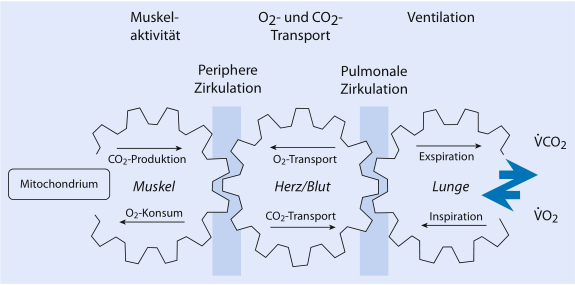
\includegraphics[scale=0.65]{Bilder/zahnraeder.png}
	\caption[3-Zahnräder-Modell mit physiologischen Interaktionen im Gasaustausch]{3-Zahnräder-Modell nach K. Wasserman: Die physiologischen Interaktionen im Austausch von \acs{CO2} und \acs{O2} zwischen Lunge, Blut und Muskelzelle~\cite{Loellgen.2010}}
	\label{pic:pic1}
\end{figure}

Ausgangspunkt der betrachteten physiologischen Prozesse ist die Atmungsventilation - also der Gasaustausch zwischen Umgebung, Lunge, Blut und Muskelzelle, wie in Abb. \ref{pic:pic1} veranschaulicht. Man kann prinzipiell zwischen "`innerer"' und "`äußerer"' Atmung bzw. peripherer und pulmonaler Zirkulation differenzieren. Die innere Atmung bezieht sich auf den molekularen Gasaustausch in den Mitochondrien. Die äußere Atmung betrifft den Transfer zwischen Blut und Lunge. Wesentlich sind hierbei die zwei in der Atemluft enthaltenen Gase \ac{CO2} und \ac{O2}.
%
\begin{equation}
RQ = \frac{\dot{V}(CO_2)}{\dot{V}(O_2)}
\label{eq:formel1}
\end{equation}
%
Das Verhältnis von \ac{VCO2} zu \ac{VO2}, der Respiratorische Quotient (\acs{RQ}), muss normalerweise getrennt für die innere und äußere Atmung betrachtet werden. Bei gesunden Menschen bzw. bei idealer Zirkulation ohne Einschränkungen auf der Strecke des Gastransfers herrscht jedoch ein Gleichgewicht ("`Steady State"')~\cite{Kroidl.2015} und das 3-Zahnräder-Modell nach Wasserman (siehe Abb. \ref{pic:pic1}) funktioniert einwandfrei. Da kardiopulmonale Defizite in der Sportmedizin ein Ausschlusskriterium für eine Spiroergometrie darstellen, wird in dieser Arbeit generell von einem Steady State ausgegangen. Der RQ wird bei der Ruhestoffwechselanalyse gemessen und deutet an, aus welchen Makronährstoffen der Körper momentan Energie bezieht. Werden ausschließlich Fette metabolisiert, liegt er bei ca. 0,7. Dies ist in absoluter körperlicher Ruhe der Fall. Liefern Kohlenhydrate die gesamte Energie, nimmt er den Wert 1 an~\cite{Kroidl.2015}. Eine steigende Kohlenhydratverbrennung wird durch zunehmende Aktivität initiiert. Darauf fußt auch der aktuelle Software-Algorithmus von cardioscan. Die damit verbundene Problematik wird in Kapitel 1.3 erläutert.

\subsection{Energiebereitstellung des Körpers}

\subsubsection{Primäre Energiebereitstellung}

Die Bewegung des menschlichen Körpers wird durch mechanische Kontraktionen der Skelettmuskulatur möglich. Hierfür dient die hydrolytische Spaltung des körpereigenen "`Brennstoffs"' \ac{ATP} zu \ac{ADP}, \ac{H+} und \ac{P} als Energiequelle:
%
\begin{equation}
ATP + H_2O \rightarrow ADP + P_i + H^+
\label{eq:formel2}
\end{equation}
%
Mit der durchschnittlichen \acs{ATP}-Konzentration im Muskel von \SIrange{5}{7}{\milli\mole\per\kg} lassen sich nur wenige Kontraktionen durchführen bzw. ein bis zwei Sekunden starke körperliche Arbeit verüben~\cite{DeMarees.1981}. Für längere Aktivität muss stetig \acs{ATP} resynthetisiert werden. Dies geschieht vorerst durch die anaerobe Reaktion von \acs{ADP}, \ac{CrP} und \acs{H+}~\cite{Heck.2006}.

\begin{equation}
ADP + CrP + H^+ \leftrightarrow ATP + Cr
\label{eq:formel3}
\end{equation}

\acs{CrP} kann mit einem Muskelgehalt von \SIrange{15}{20}{\milli\mole\per\kg} für ca. fünf bis sechs Sekunden körperlicher Last Energie liefern. Dementsprechend genügt diese Energiegewinnung nur für kurze Belastungsphasen. Mit weiterer andauernder und inkrementierter Belastung nimmt jedoch die \acs{CrP}-Konzentration sehr steil ab und der Organismus greift auf sekundäre Energiequellen zurück.

\subsubsection{Sekundäre Energiebereitstellung}

Die sekundäre Energiegewinnung kann in die aerobe sowie anaerob-laktazide ATP-Resynthese differenziert werden~\cite{Kroidl.2015}. Durch zunehmende Belastung werden mehr zusätzliche Muskelfasern rekrutiert, welche die Energie schnell benötigen und aus Glukose beziehen. Die aerobe Glykolyse setzt zuerst ein, da sie mit insgesamt ca. \SI{36}{\mole} ATP pro Glukose-Molekül sehr effektiv ist~\cite{Kroidl.2015}. Der gesamte Prozess erfolgt enzymatisch in mehreren Teilschritten und endet mit dem Anion Pyruvat~\cite{Heck.2006}. Ist genügend Sauerstoff in den Mitochondrien vorhanden, kann das Pyruvat direkt in den Citratzyklus zur ATP-Resynthese überführt werden~\cite{Rassow.2008}. Bei zunehmender Belastung und damit auch erhöhtem \acs{O2}-Verbrauch kommt mit der Zeit die oxidative Kapazität zum Erliegen und das Redox-Coenzym \acs{NADH} reichert sich in unoxidierter Form an. Für die Glykolyse wird es allerdings als oxidiertes Substrat benötigt. Damit diese fortlaufen kann, hilft sich der Organismus selbst, indem er das Pyruvat durch das Enzym \ac{LDH} zu \ac{HLa} reduziert~\cite{Rassow.2008} und die anaerob-laktazide Glykolyse aktiviert. Durch die dabei stattfindende Reoxidation des \acs{NADH}/\acs{H+} kann die Glykolyse, deren Rate bei zunehmender Muskelarbeit gesteigert werden muss, fortwähren~\cite{Heck.2006}. Bei jener entstehen aus einem Molekül Glukose zwei Moleküle \ac{HLa} bzw. \acs{H+} und \acs{La-}:

\begin{equation}
Glukose \rightarrow 2 HLa \rightarrow 2 H^+ + 2 La^-
\label{eq:formel4}
\end{equation}

Das Laktat dient zu Beginn dieser Umstellung auch als Substrat für die Rückreaktion und akkumuliert zunächst in die Skelettmuskelfasern und anschließend im Herzmuskel~\cite{Klinke.2003}. Die \acs{H+}-Konzentration steigt hingegen weiter an, sodass der Blut-pH-Wert sinkt. Dieser oftmals als "`Übersäuerung"' bezeichnete Zustand wird auch metabolische Azidose (aus lat. \textsl{acidum}: Säure) genannt~\cite{Boening.2008}. Infolgedessen wird das \acl{HCO3-}-Puffersystem des Körpers zur Aufrechterhaltung des natürlichen Säure-Base-Haushalts aktiv, wodurch das \acs{HCO3-} den \acs{H+} zu instabiler \ac{H2CO3} bindet, welche direkt zu \acs{CO2} und \acs{H2O} zerfällt~\cite{Kroidl.2015}:

\begin{equation}
HCO_3^- + H^+ \rightleftharpoons H_2CO_3 \rightleftharpoons CO_2 + H_2O
\label{eq:formel5}
\end{equation}

Das zusätzlich während dieser Prozesse entstehende \acs{CO2} muss nun mit dem \acs{CO2} aus der Energiebereitstellung über die Lunge eliminiert werden. Durch diese "`ventilatorische Kompensation"' kommt es zu einem messbaren Anstieg an exspiriertem \acs{CO2} im Verhältnis zum inspirierten \acs{O2}~\cite{Boening.2008}. Die nachweisliche \ac{CO2}-Elimination gewährleistet letztlich die ventilatorische Schwellenbestimmung.
%
\section{Spiroergometrie}

\subsection{Ventilatorische Schwellen}

Wie im Kapitel 1.2.2 aufgeführt, kann die Energiegewinnung eines Menschen grob in die Phasen aerob, aerob-anaerob und anaerob gegliedert werden~\cite{Antonutto.1995}. Die realen Zustände sind aber bei jedem Menschen sehr individuell und vermischt~\cite{Moosburger.1995}. Abhängig vom Gesundheits- oder Trainingszustand eines Menschen kann auch eine teilweise anaerobe Energiebereitstellung in Ruhe oder aber eine überwiegend aerobe bei hoher Belastung vorliegen~\cite{Skinner.1980}. Um individuell Trainingsbereiche definieren zu können, müssen diese Übergänge also zuerst bestimmt werden. Sie wurden einst als aerobe und anaerobe Schwellen deklariert~\cite{Wasserman.1973}. Da in Publikationen aus der Vergangenheit unterschiedliche Titel für die gleichen Schwellen auftauchten, wurden inzwischen mit der 1. und 2. Ventilatorischen Schwelle - abgekürzt als \acs{VT1} und \acs{VT2} - einheitliche Fachtermini festgelegt, die weitestgehend Verwendung finden~\cite{Westhoff.2012}.
\begin{table}[H]
	\centering
	\caption[Pathophysiologische Veränderungen an VT1 und VT2]{Pathophysiologische Veränderungen an VT1 und VT2~\cite{Westhoff.2012}}
	\medskip
	\begin{tabularx}{\textwidth}{X X}
		\toprule
		\textbf{VT1} & \textbf{VT2} \\
		\midrule
		\midrule
		Laktatanstieg mit Laktatpufferung zu Beginn des aerob-anaeroben Übergangs & Überschreiten des Max. Laktat-Steady-State zum Ende des aerob-anaeroben Übergangs \\
		\begin{titemize}
			\item Steigerung der Ventilation \acs{VE}
			\item Zunahme der \acs{VCO2} relativ zur \acs{VO2}
		\end{titemize}
		&\begin{titemize}
			\item Laktatexzess
			\item Metabolische Azidose
			\item Überproportionale Ventilationssteigerung
		\end{titemize}\\
		\bottomrule
	\end{tabularx}
	\label{tab:tabelle1}
\end{table}
Tab.~\ref{tab:tabelle1} listet die physiologischen Prozesse auf, die als Indikatoren für VT1 und VT2 gelten. Die \ac{VE} beschreibt das Gesamtvolumen an Luft, die pro Zeiteinheit ein- bzw. ausgeatmet wird. Sie ist ein direkter Messwert und wird in \si{\litre\per\minute} angegeben und daher auch als \ac{AMV} betitelt. Die \acs{VO2} ist das Produkt aus der \acs{VE} und der Differenz aus der Fraktion des inspirierten (\acs{FIO2}) und exspirierten Sauerstoffs (\acs{FEO2}). Da die \acs{CO2}-Konzentration in der atmosphärischen Luft vernachlässigbar klein ist, wird die \acs{VE} nur mit der \ac{FECO2} multipliziert.
%
\begin{flalign}
\dot{V}O_2 &= \dot{V}E * (FIO_2 - FEO_2)
\label{eq:formel6}\\[1em]
\dot{V}CO_2 &= \dot{V}E * FECO_2
\label{eq:formel7}
\end{flalign}

Zu Beginn einer Belastung sind Laktatproduktion und -elimination während der aeroben Glykolyse im Gleichgewicht und werden außerdem nicht gesteigert. Letzteres ändert sich jedoch bei steigender Belastung und ab Erreichen der maximalen aeroben Glykolyse mit dem ersten Anstieg der Laktatkonzentration~\cite{Antonutto.1995}. Die ventilatorische Antwort auf die Laktatzunahme ist nun das sogenannte Exzess-\acs{CO2}~\cite{Westhoff.2012}. Dieses wird zusätzlich zum normal metabolisierten \acs{CO2} exspiriert und sorgt für den überproportionalen Anstieg von \acs{VCO2} gegenüber \acs{VO2}, der ab VT1 mess- und visualisierbar wird. Daraus resultiert auch eine messbare Ventilationszunahme zum Abatmen des Exzess-\acs{CO2}~\cite{Kroidl.2015} (siehe Tab. \ref{tab:tabelle1}). Wenn die Elimination aus kapazitiven Gründen endet, der kontinuierliche Laktat-Anstieg jedoch anhält, ist das von Heck et al. geprägte Maximale Laktat-Steady-State (\acs{MLSS}) erreicht und es kommt zum Ende des aerob-anaeroben Übergangs~\cite{Heck.1985}. Sobald das \acs{MLSS} überschritten wird, setzt etwas zeitversetzt die metabolische Azidose und die weitere überproportionale \acs{VCO2}-Steigerung infolge einer Hyperventilation bei VT2 ein~\cite{Kroidl.2015}. Diese Gegebenheiten gelten allerdings nur im Falle einer störungsfreien Wechselwirkung zwischen \acs{CO2}-Gehalt im Blut und ventilatorischer Reaktion, die beispielsweise bei einer chronisch obstruktiven Lungenerkrankung (\acs{COPD}) nicht mehr funktioniert. Die ventilatorischen Schwellen werden in der Regel mit der entsprechenden Leistung in \si{\watt} oder Herzfrequenz in \si{\per\minute} angegeben.
%\clearpage

\subsection{Methoden zur Schwellenbestimmung}

\subsubsection{9-Felder-Grafik nach Prof. Karlman Wasserman}

Das wichtigste grafische Instrument der Spiroergometrie ist die 9-Felder-Grafik nach Prof. Karlman Wasserman~\cite{Wasserman.2012}. In dieser Grafik werden in neun Feldern verschiedene Messparameter des Belastungstests gegeneinander aufgetragen und in Beziehung gesetzt. Dabei besitzt jedes Feld ein eigenes Koordinatensystem und entsprechende Achsenbezeichnungen. Die Nummerierung erfolgt von links oben nach rechts unten von eins bis neun. Sowohl in der Sportmedizin als auch in der klinischen Medizin findet dieses Tool Anwendung. In der Kardiologie, Pneumologie sowie der Sportmedizin betrachtet man unterschiedliche Felder. Einige können allerdings auch Informationen für mehrere Domänen beherbergen. Die Grafik kann je nach Diagnostik-Schwerpunkt sehr komplex werden, wobei auch viele Felder mehr als zwei zu vergleichende Größen beinhalten können. In der sportmedizinischen Spiroergometrie sind, abhängig von der verwendeten Auswertungsmethode und der zu bestimmenden ventilatorischen Schwelle, nur bestimmte Felder relevant. Mittlerweile existieren hierfür einige Standards in der Sportmedizin und der Fokus wird zumeist auf die Felder 4, 5, 6 und 9 gelegt~\cite{ScharhagRosenberger.2013}. Abb.~\ref{pic:pic2} zeigt exemplarisch eine solche 9-Felder-Grafik einer sportlich aktiven Frau, die nach einem Belastungstest erstellt wurde.

\begin{figure}[H]
	\centering
	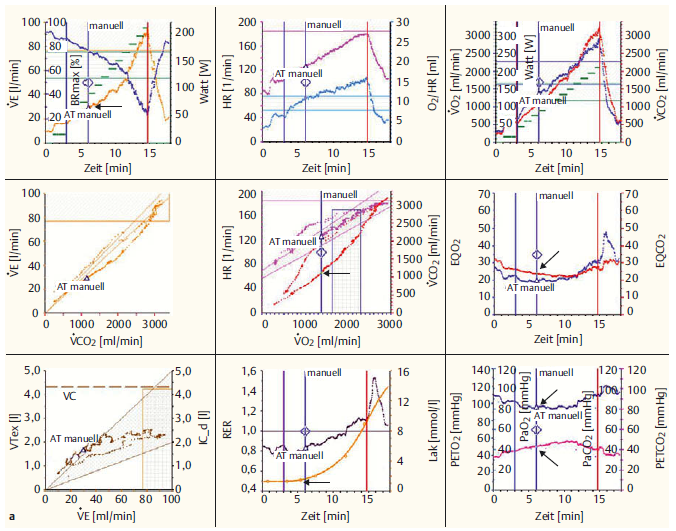
\includegraphics[width=\textwidth]{Bilder/9fieldcomplex.png}
	\caption[Beispielhafte 9-Felder-Grafik nach einer Spiroergometrie]{Beispiel einer 9-Felder-Grafik nach einer Spiroergometrie mit einer jungen sportlichen Frau mit den relevanten Feldern: 4, 5, 6 und 9.\\
	Feld 4: \acs{VE} in \si{\litre\per\minute} gegenüber \acs{VCO2} in \si{\milli\litre\per\minute}, Feld 5: \acs{HF} in \si{\per\minute} und \acs{VCO2} in \si{\milli\litre\per\minute} gegenüber \acs{VO2} in \si{\milli\litre\per\minute}, Feld 6: \acs{EQO2} und \acs{EQCO2} gegenüber der Zeit in \si{\minute}; VT1 wird mit einer vertikalen blauen Linie bzw. einer Raute und einem schwarzen Pfeil markiert. VT2 wird mit einer roten vertikalen Linie markiert.~\cite{Kroidl.2015}}
	\label{pic:pic2}
\end{figure}
%
Anhand eines Pfeils und einer vertikalen blauen Linie mit einer kleinen Raute wurde in den Feldern 1, 4, 5, 6, 8 und 9 die VT1 markiert. Eine vertikale rote Linie stellt VT2 dar. Die Plots enthalten noch weitere Cursor, die für andere diagnostische Anwendungen relevant sind. Die Felder enthalten sehr viele Informationen, weswegen die gesamte Grafik für einen Anwender ohne ausreichendes Hintergrundwissen sehr kompliziert und die Menge an Parametern und Größen sehr umfassend wird. Die 9-Felder-Grafik sich sehr gut zum Vergleich unterschiedlicher Felder und Auswertungsmethoden verwenden. Mit der ihr lassen sich Schwellenbestimmungen auf einen Blick evaluieren und auf Übereinstimmung der Werte prüfen. Allerdings müssen die Graphen zuerst manuell ausgewertet werden. Sie sind für die Zwecke und Kunden von cardioscan zu komplex, da auch zu viele Plots für die Trainingsbereichsplanung wenig relevant sind. Es wird eine Darstellung benötigt, in der lediglich die bereits algorithmisch bestimmten ventilatorischen Schwellen eingefügt werden und die keine irrelevanten Informationen beinhaltet. Der Kunde soll ein Ergebnis generiert bekommen, welches nicht mehr händisch ausgewertet werden muss und einfacher nachvollziehbar ist. Um die VT1 und VT2 zu bestimmen, existieren mehrere Verfahren. Die wissenschaftlich am erfolgreichsten angewandten Methoden wurden 2012 offiziell zusammengefasst und auf vier je Schwelle reduziert~\cite{Westhoff.2012}. Da die Evaluation aller aufgeführten Methoden zeitlich zu umfangreich wäre, wird sich in dieser Arbeit nur auf die jeweils zwei renommiertesten Methoden konzentriert. Tab.~\ref{tab:tabelle2} listet diese gegenübergestellt für die VT1 und VT2 auf und nennt die relevanten Messwerte sowie die entsprechenden Plots der 9-Felder-Grafik.
%
\begin{table}[H]
	\centering
	\caption{Ausgewählte Methoden zur Bestimmung von VT1 und VT2}
	\medskip
	\begin{tabularx}{\textwidth}{X X}
		\toprule
		\textbf{VT1} & \textbf{VT2} \\
		\midrule
		\midrule
		\begin{titemize}
			\item V-Slope-Methode: erster überproportionaler Anstieg der \acs{VCO2} gegenüber der \acs{VO2} (Feld 5)
			\item Anstieg des \ac{EQO2} ohne gleichzeitigen Anstieg des \ac{EQCO2} (Feld 6)
		\end{titemize}
		&\begin{titemize}
			\item überproportionaler Anstieg der \acs{VE} gegenüber der \acs{VCO2} (Feld 4)
			\item Anstieg des \ac{EQCO2} (Feld 6)
		\end{titemize}\\
		\bottomrule
	\end{tabularx}
	\label{tab:tabelle2}
\end{table}
%
\subsubsection{Bestimmung der VT1}

\begin{figure}[H]
	\centering
	\begin{subfigure}[c]{0.45\textwidth}
		\centering
		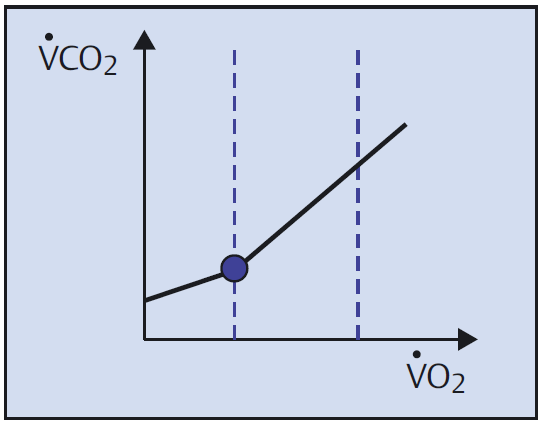
\includegraphics[width=50mm]{Bilder/vslope.png}
		\subcaption[Schematische Darstellung der V-Slope-Methode]{Schematische Darstellung der V-Slope-Methode, bei der die \acs{VCO2} gegen die \acs{VO2} aufgetragen wird}
		\label{subpic:pic5}
	\end{subfigure}%
	\hfil
	\begin{subfigure}[c]{0.45\textwidth}
		\centering
		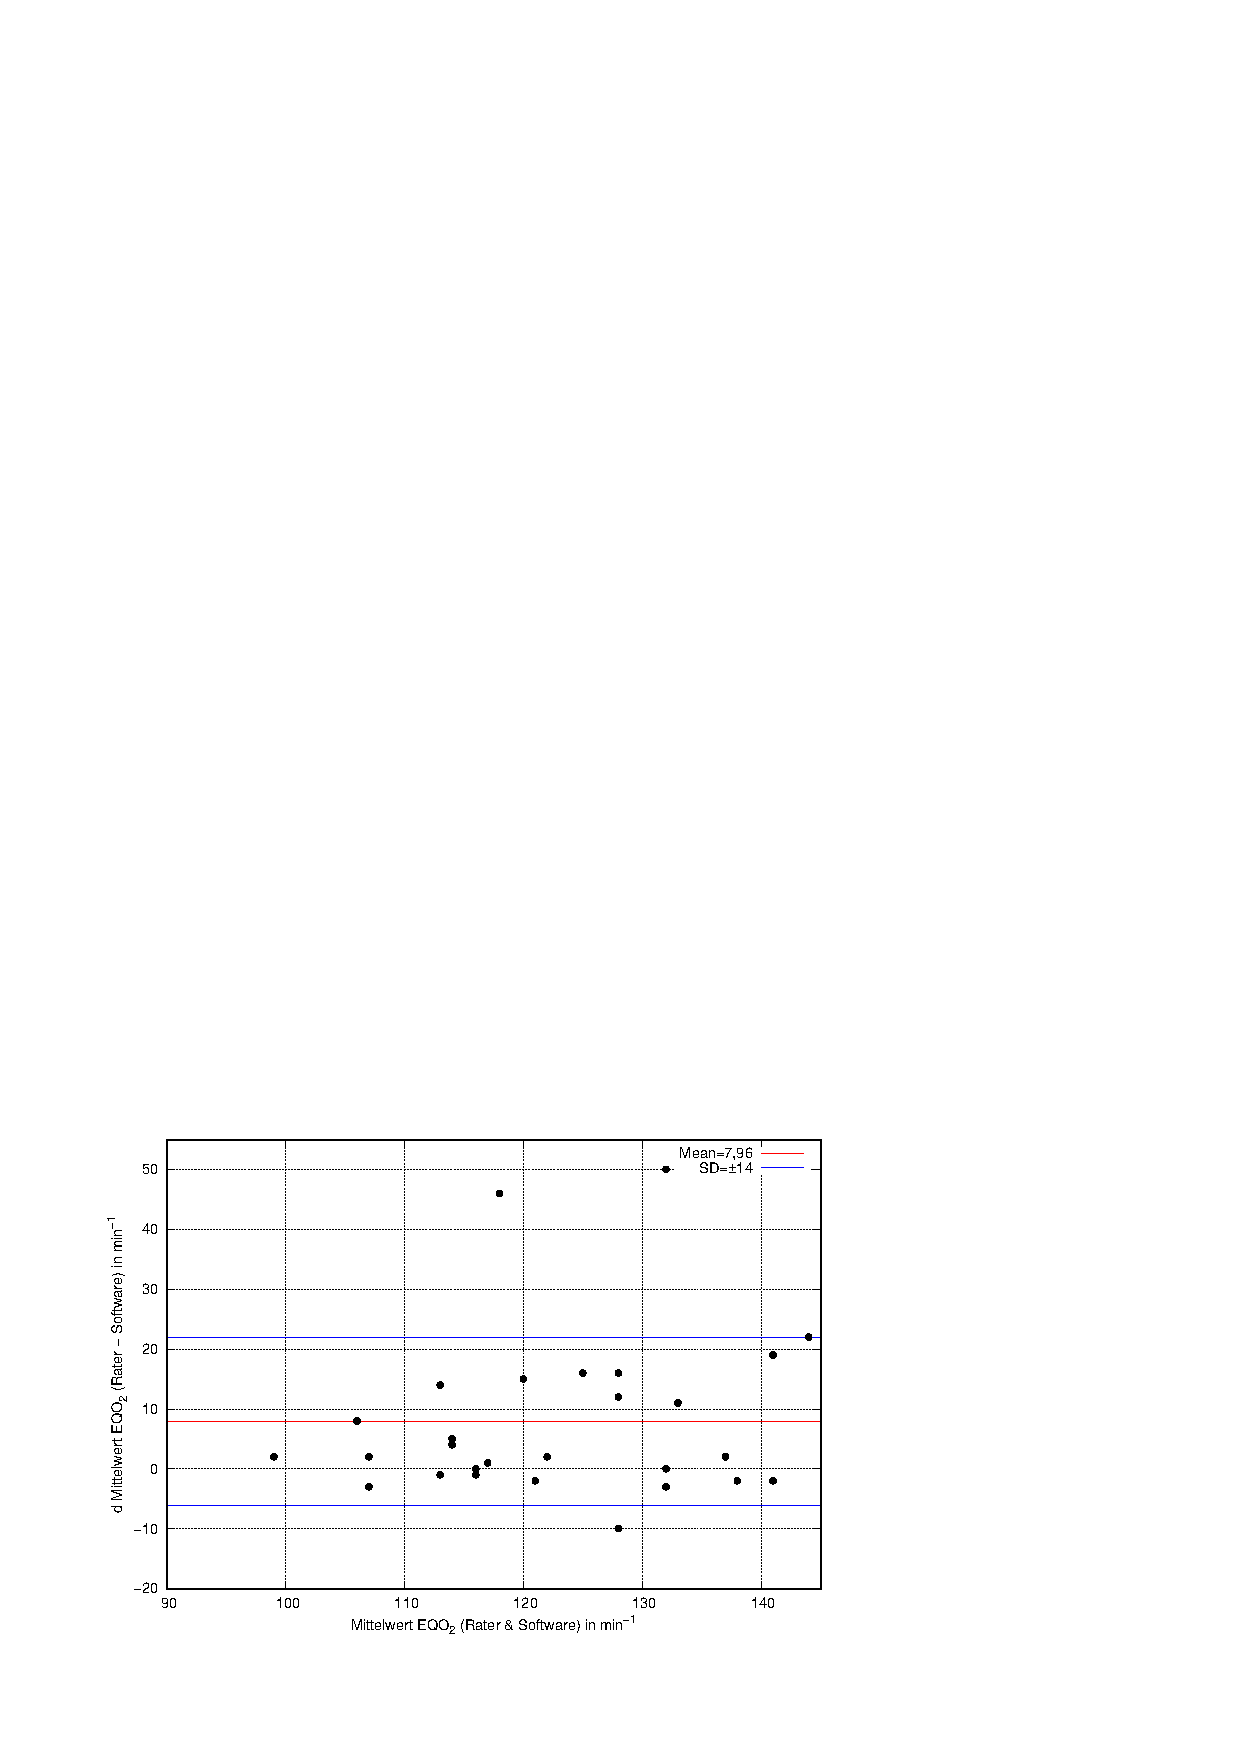
\includegraphics[width=50mm]{Bilder/eqo2.png}
		\subcaption[Schematische Darstellung des \acs{EQO2}]{Schematische Darstellung des \acs{EQO2}; Das Verhältnis aus der \acs{VE} und der \acs{VO2} wird gegenüber der Zeit oder der Leistung \acs{WL} geplottet}
		\label{subpic:pic6}
	\end{subfigure}
	\caption[Methoden zur grafischen Bestimmung der VT1]{Methoden zur grafischen Bestimmung der VT1; Die VT1 wird durch die erste vertikale Linie und den blauen Punkt markiert. Die zweite vertikale Linie deutet VT2 an~\cite{Kroidl.2015}}
	\label{pic:pic4}
\end{figure}

Die erste Methode zur Bestimmung der VT1 ist die Begutachtung des sogenannten "`V-Slopes"' in Feld 5 nach Beaver et al.~\cite{Beaver.1986}. Die Nomenklatur bezieht sich auf den Vergleich zwischen der \acs{VCO2} und der \acs{VO2}, welches beide Volumengrößen sind, sowie die sich ändernde Steigung (engl. \textsl{slope}) des Graphen. Dabei geht es um die Identifizierung charakteristischer Knickpunkte als Indikator für das Exzess-\acs{CO2}. Dieser grafische Vergleich der Flows an \acs{CO2} und \acs{O2} ist sehr stark vereinfacht und idealisiert als schematisches Beispiel in Abb.~\ref{subpic:pic5} zu sehen. Ebenfalls anwendbar ist die gleichzeitige Analyse der Atemäquivalente \acs{EQCO2} und \acs{EQO2} in Relation zur Zeit in \si{\minute} oder alternativ der Belastung \acs{W} (bzw. \acs{WL}) in \si{\watt} in Feld 6. Mathematisch werden diese durch das Verhältnis aus \acs{VE} und dem Flow des jeweiligen Gases definiert. Die Atemäquivalente sind einheitslos.
%
\begin{flalign}
EQO_2 = \frac{\dot{V}E}{\dot{V}O_2}  &\hspace{2cm} EQCO_2 = \frac{\dot{V}E}{\dot{V}CO_2}
\label{eq:formel8}
\end{flalign}
%
Dieses Schema ist vereinfacht in Abb.~\ref{subpic:pic6} zu sehen. Anhand der linken gestrichelten Linien und den blauen Punkten in Abb. \ref{pic:pic4} ist VT1 markiert. Bei VT1 ist erkennbar, dass \acs{VCO2} gegenüber \acs{VO2} durch das zusätzliche Exzess-\acs{CO2} aus der Laktatpufferung stärker ansteigt. Wo eine zweite deutliche Zunahme von \acs{VCO2} zur Kompensation der metabolischen Azidose erkennbar ist, kann ggf. je nach Qualität des Graphen auch VT2 gekennzeichnet werden, weshalb in der Abbildung durch die rechte gestrichelte Linie auch VT2 angedeutet ist. Dies wird allerdings lediglich für Vergleiche mit anderen Methoden getan und zählt nicht als gängige VT2-Methode. Die Atemäquivalente \acs{EQCO2} und \acs{EQO2} beschreiben, wie viel geatmet werden muss, um einen Liter \acs{O2} aufzunehmen bzw. \acs{CO2} abzugeben. Der Tiefpunkt der \acs{EQO2}-Kurve wurde 1958 von Hollmann als Punkt des optimalen Wirkungsgrades (\acs{POW}) deklariert, welcher sich mit VT1 deckt~\cite{Kroidl.2015}. Auch hier sind anhand der gestrichelten Linien beide Schwellen (VT1 links, VT2 rechts) markiert. Danach beginnt die Laktatbildung und die Ventilation nimmt im Zuge der \acs{CO2}-Elimination zu, wodurch vorerst nur die \acs{EQO2}-Kurve beginnt, anzusteigen.

\subsubsection{Bestimmung der VT2}

Wie in Abb.~\ref{pic:pic5} durch die rechte gestrichelte Linie zu sehen, ist die VT2 ebenfalls in Feld 6 durch Betrachtung der Atemäquivalente bestimmbar. Dazu wird jedoch die \acs{EQCO2}-Kurve analysiert, wie schematisch in Abb.~\ref{subpic:pic7} verdeutlicht. Diese nimmt für üblich eine charakteristische "`Badewannenform"' an~\cite{Kroidl.2015}.
%
\begin{figure}[H]
	\centering
	\begin{subfigure}[c]{0.45\textwidth}
		\centering
		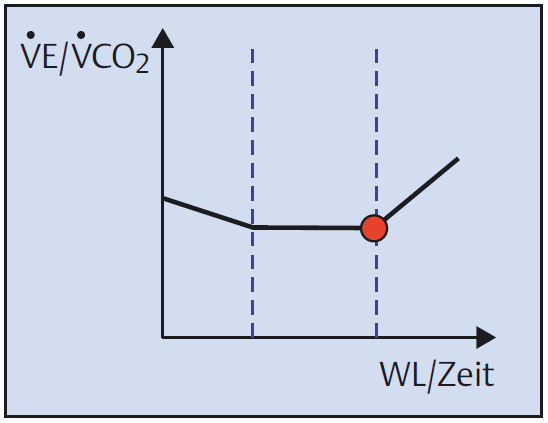
\includegraphics[width=50mm]{Bilder/eqco2.png}
		\subcaption[Schematische Darstellung des \acs{EQCO2}]{Schematische Darstellung des \acs{EQCO2}; Das Verhältnis aus der \acs{VE} und der \acs{VO2} wird gegenüber der Zeit oder Leistung \acs{WL} geplottet}
		\label{subpic:pic7}
	\end{subfigure}%
	\hfil
	\begin{subfigure}[c]{0.45\textwidth}
		\centering
		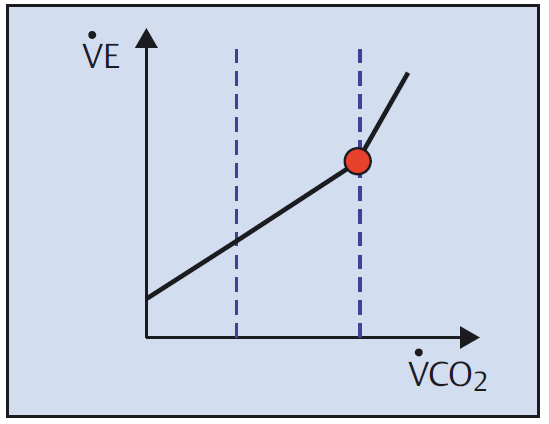
\includegraphics[width=50mm]{Bilder/field4.png}
		\subcaption[Schematische Darstellung der \acs{VE} relativ zur \acs{VCO2}]{Schematische Darstellung des grafischen Vergleichs der \acs{VE} relativ zur \acs{VCO2}; Analogie zum V-Slope}
		\label{subpic:pic8}
	\end{subfigure}
	\caption[Methoden zur grafischen Bestimmung der VT2]{Methoden zur grafischen Bestimmung der VT2; Die VT2 wird durch die zweite vertikale Linie und den orangen Punkt markiert. Die erste vertikale Linie deutet VT1 an~\cite{Kroidl.2015}}
	\label{pic:pic5}
\end{figure}
%
In Abb. \ref{pic:pic5} wird VT2 durch die rechte Linie und den orangefarbenen Punkt markiert. Bei Analyse des \acs{EQCO2} wird sie an dem Punkt gesetzt, an dem \acs{EQCO2} deutlich sichtbar ansteigt. Dies ist in Abb. \ref{subpic:pic7} erkennbar. Dies stellt die Kompensation der metabolischen Azidose aufgrund des Ventilationsanstiegs, der sich auch in \acs{VCO2} widerspiegelt, dar. Als Goldstandard für die VT2-Bestimmung wird die Gegenüberstellung von \acs{VE} und \acs{VCO2} in Feld 4 behandelt~\cite{ScharhagRosenberger.2013}. Dabei wird auf Erkenntnisse von Meyer et al. verwiesen, die mit dieser Methode bei einer Vielzahl an Probanden die VT2 (damals "`anaerobe Schwelle"') bestimmen konnten~\cite{Meyer.2005}. In Abb.~\ref{subpic:pic8} ist diese Methode vereinfacht visualisiert. Diese Grafik weist Analogien zum V-Slope auf, da auch zwei Flows miteinander verglichen und auch hier die Schwellen mithilfe von Knickpunkten bestimmt werden. An der rechten gestrichelten Linie und dem orangen Punkt auch dort die VT2 zu sehen, welche der zur Azidose-Kompensation einsetzenden Hyperventilation bei ausgelastetem Bicarbonat-Puffer folgt~\cite{ScharhagRosenberger.2010}.\\
Der V-Slope und der Vergleich der \acs{VE} zur \acs{VCO2} werden häufig als allgemeine Goldstandards bezeichnet~\cite{ScharhagRosenberger.2013}. Dennoch wurde bereits von Friederike Scharhag-Rosenberger~\cite{ScharhagRosenberger.2010} und Wilfried Kindermann~\cite{Kindermann.2004} vom Institut für Sport- und Präventivmedizin Saarbrücken festgestellt, dass ansteigende Intensitäten bei Stufentests für Artefakte sorgen können und deshalb stets differenziert ausgewertet werden müssen. Generell sollten unterschiedliche Methoden angewandt und zur Auswertung kombiniert werden, um Vergleiche innerhalb einer individuellen Diagnostik anstellen zu können~\cite{ScharhagRosenberger.2010}.
%\clearpage
\section{Problemstellung \& Ziele der Arbeit}

Die Bestimmung der ventilatorischen Schwellen in der Leistungsdiagnostik ist ein modernes und häufig empfohlenes Verfahren zur Trainingsplanung und daher für cardioscan eine sinnvolle Technik. Momentan nutzt die Firma einen Algorithmus, der vom RQ abhängig ist. Die VT2 wird dort gesetzt, wo dieser den Wert eins erreicht. Begründet wird diese Verfahrensweise dadurch, dass Fettsäuren in körperlicher Ruhe den oxidativen Hauptenergielieferanten verkörpern, der RQ dann normalerweise bei ca. 0,7 liegt und mit zunehmender Belastung langsam ansteigt. Diefenthaeler et al.~\cite{Diefenthaeler.2017} und Zagatto et al.~\cite{Zagatto.2012} konnten dies in ihren Studien untermauern. Leti et al. hingegen machten die Beobachtung, dass die Belastungsintensität bei RQ~=~1 deutlich von der objektiv mit VT2 assoziierten Intensität abwich~\cite{Leti.2012}. Dem sind besonders Trainingszustand sowie Belastungsart und -protokoll zugrundeliegend. Erschwert wird zusätzlich dadurch, dass der Respiratorische Quotient (\acs{RQ}) auf unterschiedliche Weise, z.B. durch kohlenhydrathaltige Ernährung, akut beeinflussbar ist~\cite{ScharhagRosenberger.2010}. cardioscan arbeitet mit Stufenprotokollen und nutzt hauptsächlich Fahrradergometer. Daraus können ebenfalls Abweichungen bei den Trainingszonen resultieren, wenn beispielsweise Laufathleten, die nicht häufig Fahrrad fahren, relativ frühzeitig muskulär ausbelastet sind, obwohl der RQ noch unterhalb von 1 liegt. Eine kardiorespiratorische Ausbelastung läge somit noch nicht vor und die VT2 wäre faktisch noch nicht erreicht~\cite{Tzvetkov.2008}. Zur Bestimmung der VT2 ist das Erreichen des Maximums jedoch unabdingbar~\cite{ScharhagRosenberger.2013}. Gemäß der Literaturempfehlungen wurden daher mehrere alternative Verfahren ausgewählt.\\
Zur Bestimmung der VT1:
%
\begin{itemize}
	\item V-Slope-Methode durch Analyse der \acs{VCO2} zur \acs{VO2}
	\item Äquivalent-Methode und alleiniger Anstieg des \acs{EQO2}
\end{itemize}
%
Zur Bestimmung der VT2:
%
\begin{itemize}
	\item Identifizierung des Anstiegs der \acs{VE} gegenüber der \acs{VCO2}
	\item Äquivalent-Methode und Anstieg des \acs{EQCO2}
\end{itemize}
%
Als Referenz für die VT2 wurde bei den Testmessungen die momentane Methode RQ~=~1 angewandt.\\
Im Rahmen der Arbeit werden mithilfe der Messungen folgende Fragen behandelt:
%
\begin{enumerate}
	\item Eignet sich der metabolicscan zur Bestimmung ventilatorischer Schwellen?
	\item Mit welcher Methode können die Schwellen optimal bestimmt werden?
	\item Ist eine genauere Bestimmung der VT2 mit den neuen Methoden möglich?
\end{enumerate}
%
Ziel dieser Arbeit war die Durchführung von Testmessungen sowie Evaluierung der genannten Methoden mit dem metabolicscan. Hierfür bestimmten mehrere zwei Personen und ein Algorithmus unabhängig voneinander beide Schwellen. Deren Auswertungen wurden miteinander verglichen und die Korrelation der Ergebnisse analysiert.
\clearpage
	\chapter{Methode}

Zur Bearbeitung der Fragestellung wurde im Umfang dieser Arbeit ein firmeninternes Pilotprojekt durchgeführt, bei dem spiroergometrische Testmessungen mit unterschiedlichen internen und externen Probanden stattfanden. Im Vorwege wurden Einschluss- und Ausschlusskriterien sowie Bedingungen zur Vorbereitung erarbeitet, welche bei allen Testpersonen gleichermaßen eingehalten wurden. Eingeladen waren gesunde Menschen zwischen 18 und 60 Jahren, zu denen Sportler und Nicht-Sportler sowie Raucher und Nichtraucher zählten. Die Daten der Teilnehmer des Projektes sind unter Kapitel 2.5 aufgeführt. Mit den Messwerten wurden Grafiken generiert, anhand derer die ventilatorischen Schwellen zu bestimmen waren.

\section{Material \& Testaufbau}

Für die Tests wurde das \textsl{motion cycle 200med} der Firma \textsl{Emotion Fitness} genutzt, welches seriell mit einem Laptop und der \acs{CCPS} verbunden wird. Zur Abklärung der kardialen Gesundheit wurde der \textsl{cardioscan cs-3 effect} genutzt. Dies ist das firmeneigene MPG-zertifiziert Medizingerät zur Erstellung von Ruhe-Elektrokardiogrammen (\acs{EKG}) mittels tetrapolarer Klebe-Elektroden, mit dem die \ac{HF} in Ruhe und der \ac{CSI} erhoben werden. Für alle Tests wurde ein kalibriertes Modell des metabolicscan genutzt. Die Respirationsmessung erfolgt beim metaboliscan durch eine Atemeinheit, welches über ein Kabel und einen Probenschlauch mit der Haupteinheit des Gerätes verbunden ist. Dieses sowie der Laptop und der cs-3 effect stehen darum auf einem Tisch in unmittelbarer Nähe zum Ergometer. Die Atemeinheit wird vor jeder Messung mit einem unbenutzten antibakteriellen Polypropylen-Filter des Herstellers \textsl{GVS} und einem dazugehörigen flexiblen Elastomer-Mundstück versehen. Jenes dient der Möglichkeit, das Atemmodul mit der Kiefermuskulatur festzuhalten, sodass die Hände während einer Messung am Ergometer bleiben können.

\subsection{Funktionsweise des metabolicscan}

Der metabolicscan besteht aus zwei Modulen: dem Atemmodul und der Haupteinheit. Im Atemmodul des metabolicscan ist ein Flowsensor\footnote{Technische Daten: siehe Anhang A} verbaut. Dieser misst in direkter Nähe zum Mund die Strömungsgeschwindigkeit der Inspirations- bzw. Exspirationsluft in einem Bereich von $\pm$\SI{300}{S\litre\per\minute} mit einer Abtastrate von einer Millisekunde. Mithilfe einer mathematischen Integration über der Zeit wird anschließend das Strömungsvolumen berechnet. \acs{O2}- und \acs{CO2}-Sensor\footnote{Technische Daten: siehe Anhang B} sind in der separaten Haupteinheit implementiert. Sie bilden ein optimal aufeinander abgestimmtes Modul und müssen daher für die Messung nicht zeitlich synchronisiert werden. Ein Anteil der Luft wird am Ende des Flowsensors über den Probenschlauch durch die integrierte Pumpe des \acs{CO2}-Sensors angesaugt. Die Funktion des \acs{CO2}-Sensors basiert auf Messung der Infrarotlichtabsorption durch \acs{CO2}, die im Spektralbereich von \SIrange{4,2}{4,3}{\micro\metre} besonders stark ist. Er eignet sich für eine \ac{AF} bis zu \SI{150}{\per\minute}, was ausreicht, da diese bei einer Spiroergometrie selten höher als \SI{60}{\per\minute} ansteigt~\cite{Hollmann.2006}. Anschließend wird die angesaugte Luft zum galvanischen \acs{O2}-Sensor geleitet. Dieser hat im Konzentrationsbereich von 0 bis 40 \% eine Genauigkeit von $\pm$~ (1~ \%\textsubscript{abs} + 1 \%\textsubscript{rel}), solange die \acs{AF} \SI{60}{\per\minute} nicht überschreitet.

\begin{figure}[H]
	\centering
	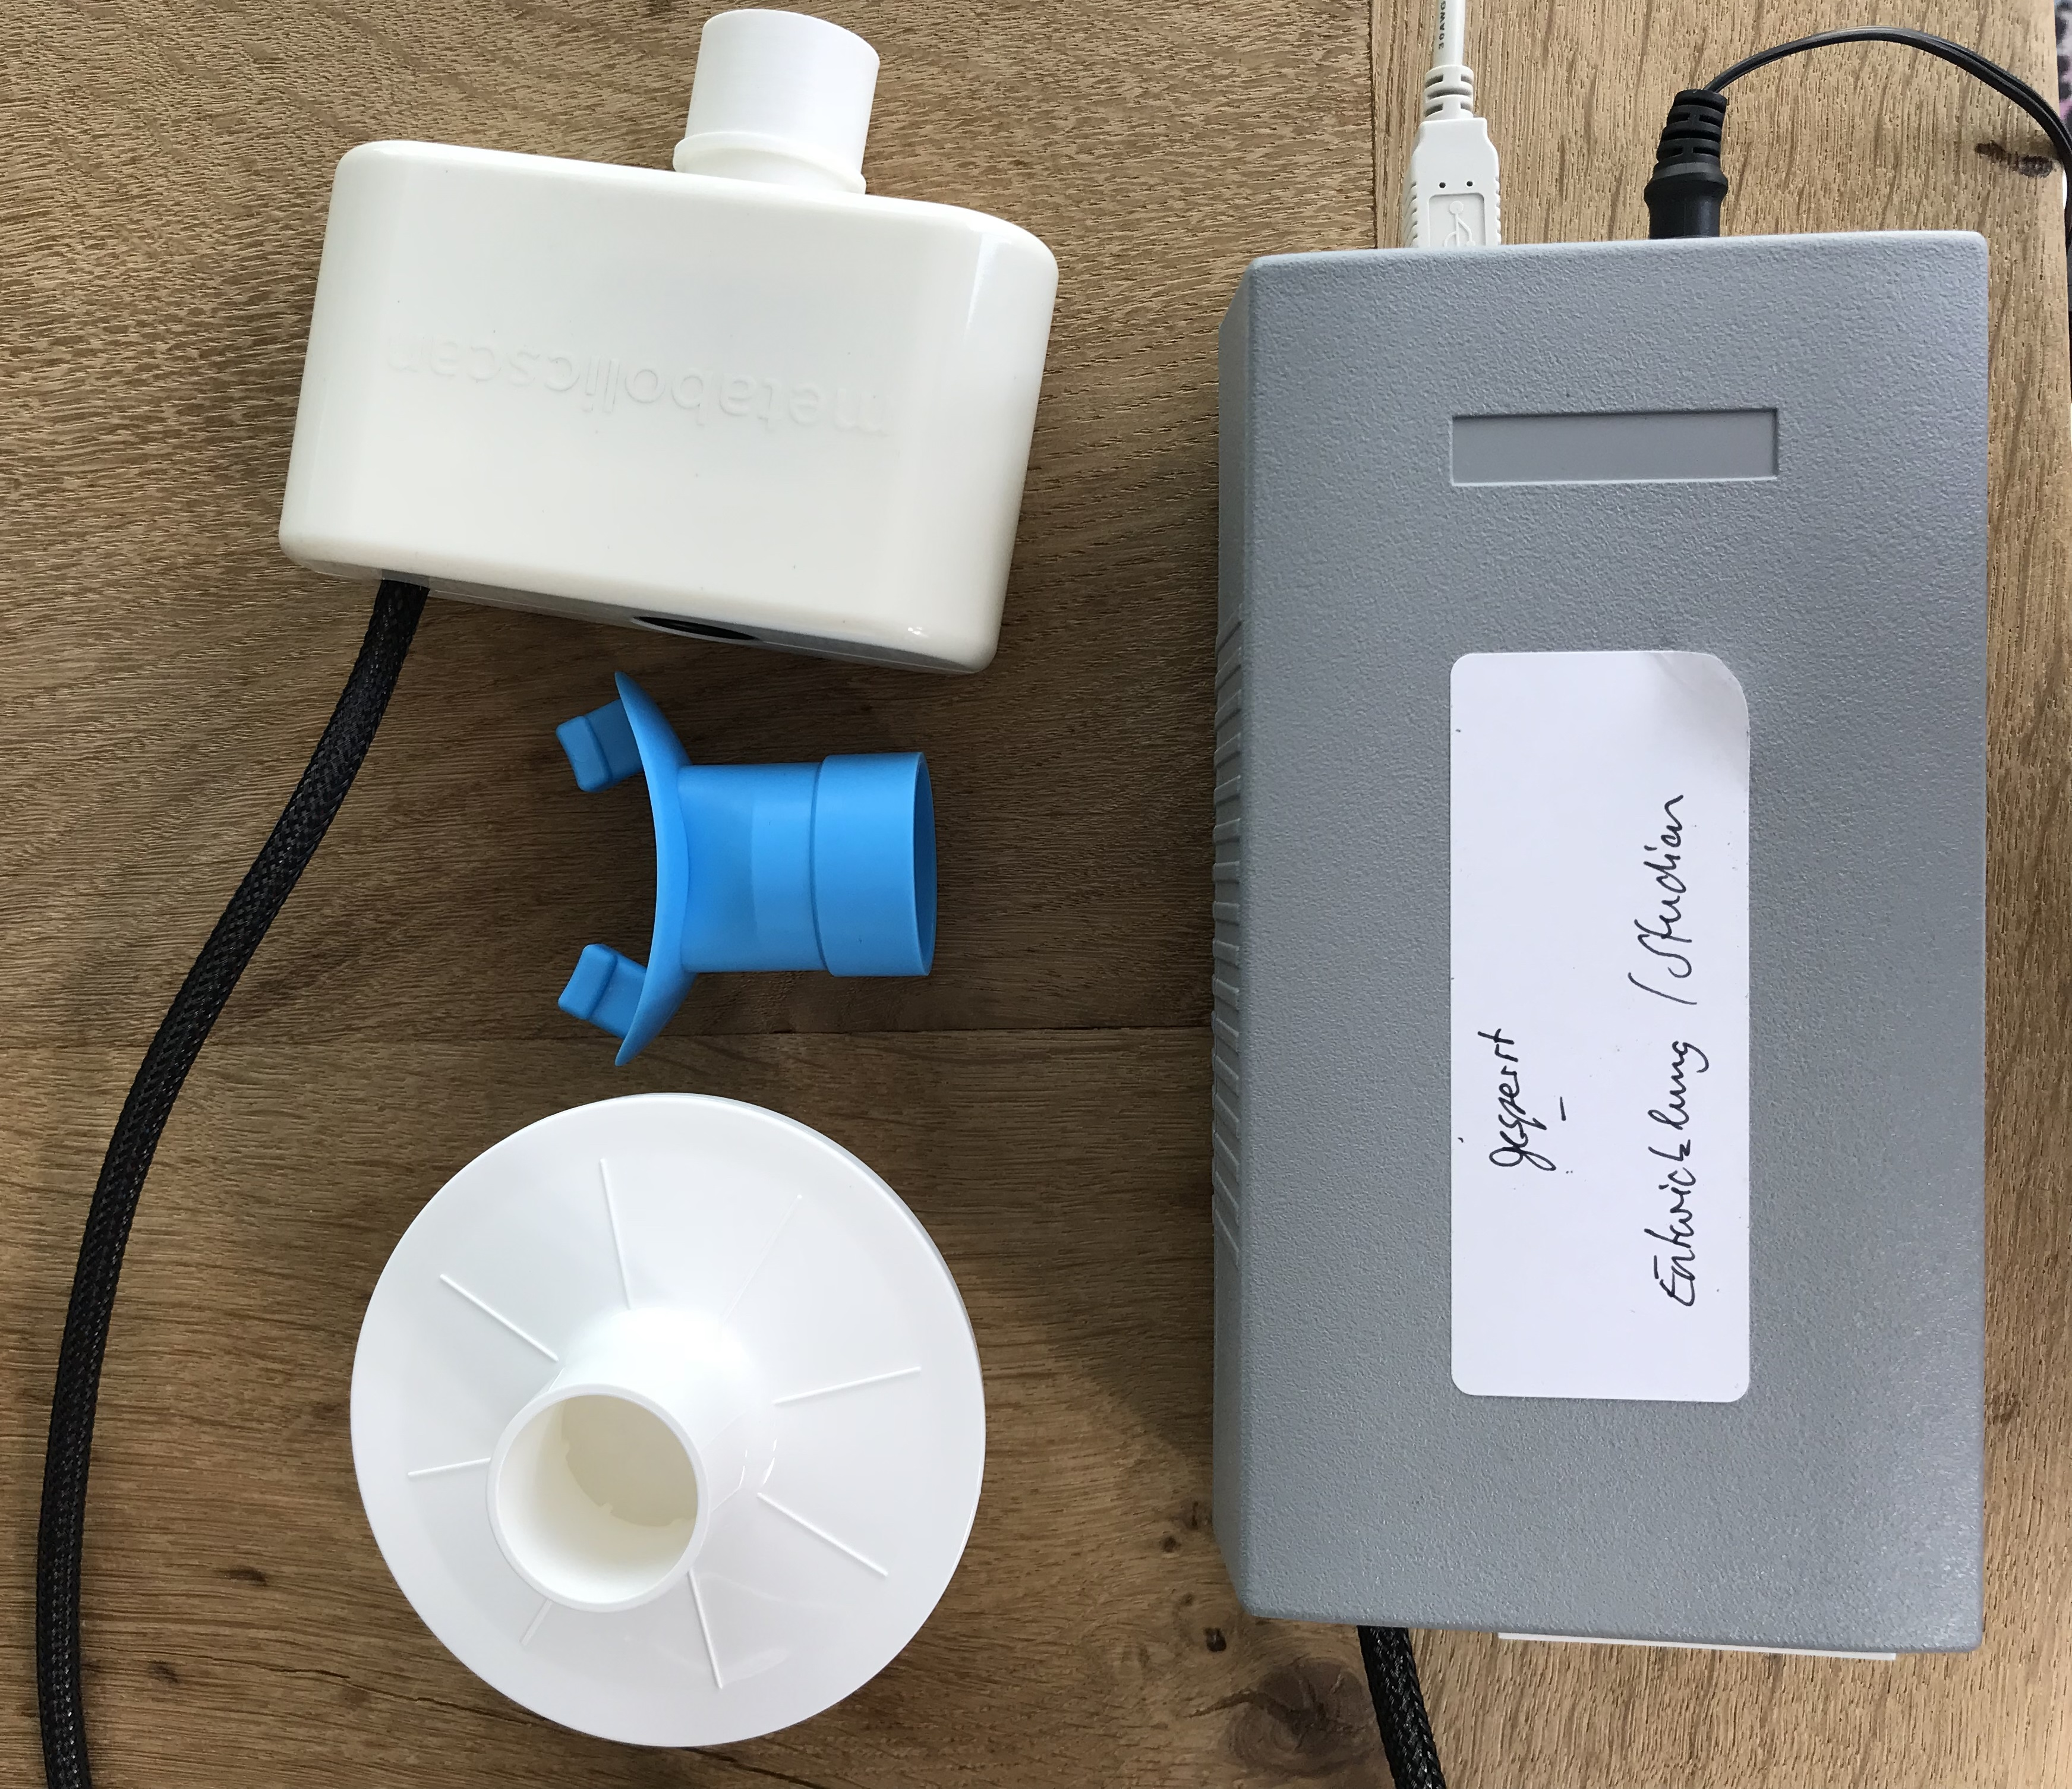
\includegraphics[width=100mm]{Bilder/mbs.jpg}
	\caption[metabolicscan: Haupteinheit, Atemmodul, Filter und Mundstück]{metabolicscan: Haupteinheit (rechts), Atemmodul (oben links), Filter (unten links) und Mundstück (blau)}
	\label{pic:pic9}
\end{figure}

\subsection{Messbedingungen}

Um gleichwertige Grundbedingungen zu schaffen, fanden alle Messungen in demselben Raum statt und es wurde darauf geachtet, dass die Raumtemperatur zwischen \SIlist{18;22}{\degreeCelsius} betrug, da diese sich auf die Herzfrequenz und Laktatakkumulation auswirken kann~\cite{Marino.2001}. Außerdem wurde der Raum vor jedem Test gut durchlüftet, um den \acs{CO2}-Anteil der Luft zu minimieren. Der metabolicscan wurde mindestens zehn Minuten vor dem ersten Test eingeschaltet, da sich die Sensoren kalibrieren und aufheizen müssen.
Als generelle Ausschlusskriterien für Probanden waren akute fiebrige Infekte, Herz-Kreislauf-Erkrankungen, chronische Atemwegserkrankungen (z.B. COPD) und Schwangerschaft festgelegt. Alle Teilnehmer erhielten bei Terminvergabe einen Informationsbogen, in dem sie unter anderem darüber aufgeklärt wurden, dass am Vortag auf anstrengende Sporteinheiten verzichtet werden sollte und ab zwei Stunden vor der Messung keine Mahlzeiten mehr eingenommen werden durften, da vor allem zuckerhaltige Lebensmittel kurz vor einer Messung neben dem RQ auch den Grund-Laktat-Spiegel erhöhen und somit das Messergebnis verfälschen~\cite{Ivy.1981}. Auch auf Koffein sollte in diesem Rahmen wegen eventueller Entzugserscheinungen verzichtet werden~\cite{Kroidl.2015}. Beim Fahrradergometer kann die Belastungsintensität neben der voreingestellten Leistung auch noch durch die Trittfrequenz beeinflusst werden. Damit die Intensität möglichst artefaktfrei gemäß des Belastungsprotokolls inkrementiert wird, sollte deshalb jeder Proband eine Trittfrequenz zwischen \SIlist{70;90}{\per\minute} beibehalten~\cite{Wonisch.2008}.

\section{Durchführung der Messungen}

\subsection{Vorbereitung \& Erwartungswerte}

Unmittelbar vor einem Test wurden die Probanden ein weiteres Mal über die Durchführung sowie eventuelle Risiken informiert und hatten eine Einwilligungserklärung zu unterzeichnen. Anschließend wurde ein Anamnesebericht ausgefüllt. Dafür wurden zunächst die Körpergröße sowie das Körpergewicht mithilfe der Ultraschallmessstation \textsl{seca 287} ermittelt. In Folge eines kurzen Interviews wurde der Trainings- und Gesundheitszustand der Person notiert. Mit dem cs-3 effect wurde ein zweiminütiges Ruhe-\acs{EKG} erstellt. Danach konnten durch die \acs{CCPS} Auffälligkeiten der \acs{HF} und des Herzrhythmus im Ruhezustand detektiert und betroffene Personen ggf. abgelehnt werden. Zur Erfassung der \acs{HF} während der Belastungsphase wurde ein Pulsgurt der Firma \textsl{Polar} angelegt, welcher mit dem Ergometer und der Software kommuniziert. Der Sattel des Ergometers war individuell für jeden Probanden ungefähr auf Hüfthöhe zu positionieren, sodass der Kniewinkel nicht mehr als $90$ \textdegree{} betrug, da dies eine höhere muskuläre Belastung beim Treten bewirken kann.

\subsubsection{Berechnung der maximalen Soll-Belastungsintensität}

Wie die Bezeichnung "`Leistungsdiagnostik"' bereits suggeriert, ist es enorm wichtig, dass die gemessene Person bis an ihr individuelles Leistungsmaximum gelangt, damit beide Schwellen vollwertig identifiziert werden können. Aus diesem Grund wurde vor einem Test ein individuelles Belastungsprotokoll für den Probanden erstellt. Den ersten Schritt stellte die Berechnung der maximalen Soll-Belastungsintensität in \si{\watt} dar, mit dem ein mindestens zu erwartender Wert bestimmt werden konnte. In der \ac{SHIP} sowie Studien nach Jones wurden Formeln für die Berechnung der Soll-Belastung erarbeitet. Nach SHIP~\cite{Koch.2009}:
%
\begin{flalign}
W_{max} (\male) &= -103,512 - 1,5766 * age + 2,2114 * \left\lbrace h\right\rbrace  \text{in \centi\metre} - 0,1198 * \left\lbrace m\right\rbrace \text{in \kilogram}
\label{eq:formel9}\\[1em]
W_{max} (\female) &= -80,628 - 0,7698 * age + 1,4038 * \left\lbrace h\right\rbrace \text{in \centi\metre} + 0,2873 * \left\lbrace m\right\rbrace \text{in \kilogram}
\label{eq:formel10}
\end{flalign}

Nach Jones (inklusive tolerierter Streuung von $\pm$18 \%)~\cite{Kroidl.2015}:
%
\begin{flalign}
W_{max} (\male) &= (2526 * \left\lbrace h\right\rbrace \text{in \metre} - 9,08 * age - 2759) * 0,163
\label{eq:formel11}\\[1em]
W_{max} (\female) &= (950 * \left\lbrace h\right\rbrace \text{in \metre} - 9,21 * age - 756) * 0,163
\label{eq:formel12}
\end{flalign}

Die folgenden Rechnungen zeigen die Anwendung bei einer weiblichen Probandin (w, 19) als Beispiel:
%
\begin{flalign*}
W_{max} &= -80,628 - 0,7698 * 19 + 1,4038 * 172\centi\metre - 0,2873 * 67\kilogram = 166\watt\\[1em]
W_{max} &= (950 * 1,72\metre - 9,21 * 19 - 756) * 0,163 = 181\watt \pm18\%
\end{flalign*}

Die Differenz zwischen den beiden Sollwerten ist mit \SI{15}{\watt} recht gering. Da beide Rechnungen offiziell empfohlen werden, wurde in dieser Arbeit dennoch bei allen Messungen mit beiden Formeln gerechnet und dann ein Mittelwert aus jedem Ergebnis gebildet~\cite{Kroidl.2015}. Für diese Probandin betrüge die maximale Belastungsintensität, welche abhängig von Alter und Körperdaten auch im untrainierten Zustand bewältigt werden kann, somit theoretisch \SI{174}{\watt}. Der Trainingszustand einer Person wurde bei der Bestimmung des Belastungsprotokolls berücksichtigt.

\subsubsection{Individuelles Belastungsprotokoll}

Mithilfe der maximalen Belastungsintensität wurde anschließend das Stufenprotokoll festgelegt. Die Dauer einer Belastungsstufe betrug zwei Minuten, wobei während der letzten \SI{30}{\second} einer Stufe die respiratorischen Werte erfasst wurden. Empfehlungen für Tests auf Fahrradergometern liegen zwischen \SIlist{7;26}{\minute} Gesamtdauer~\cite{Midgley.2008}. Darum wurde mit $n = 6$ ein Minimalwert für die zu bewältigenden Stufen \`{a} \SI{2}{\minute} bestimmt, da die Dauer eines Test somit \SI{12}{\minute} betrug und die Gefahr einer unzureichenden kardiorespiratorischen Ausbelastung reduziert wurde~\cite{Wonisch.2008}. Es war allerdings bei trainierten Personen davon auszugehen, dass sie die Soll-Belastung übertreffen und daher mehr als sechs Stufen ertragen. Deshalb wurde diese Zahl nur als ungefährer Richtwert verwendet. Als Inkrement wurde das Schema der \ac{WHO} mit \SI{25}{\watt} Steigerung je Stufe eingestellt. Dieser Standard galt für untrainierte wie trainierte Probanden, da hiermit eine Ausbelastung weitestgehend erreichbar sei~\cite{Trappe.2000}. Um die passende Anfangsbelastung zu bestimmen, wurde beispielsweise nach folgender Rechnung gearbeitet:

\begin{equation}
W_{Start} = W_{max} \text{(berechnet)} - 6 * 25 \watt 
\label{eq:formel13}
\end{equation}

Für die vorherige Beispielprobandin (w, 19) gilt dann:

\begin{equation*}
W_{Start} = 174\watt - 6 * 25\watt = 174\watt - 150\watt = 24\watt
\end{equation*}

Da diese Intensität allerdings nur minimal über der Leerlast durch den Eigenwiderstand des Ergometers mit \SI{15}{\watt} liegt, wurde bei dieser Probandin sowie bei allen weiteren sportlich aktiven Personen das Schema des Bundesausschusses Leistungssport (\acs{BAL}) angewandt und eine Anfangsbelastung von \SI{50}{\watt} oder höher gewählt~\cite{Trappe.2000}. Dennoch wurde stets darauf geachtet, jene nicht zu überschätzen und damit eine muskuläre Erschöpfung vorzuziehen. Das Protokoll wurde schließlich in einen Softwaredialog der \acs{CCPS} eingepflegt. In dem Dialog war die Einstiegsbelastung gemäß der Berechnungen mit Berücksichtigung des Trainingszustands, das Inkrement mit \SI{25}{\watt}, die Stufendauer mit \SI{1,5}{\minute} sowie das Messintervall mit \SI{30}{\second} einzutragen. Generell ist bei keinem Menschen vorhersehbar, welche Anfangsbelastung und welches Inkrement optimal sind. Neben der körperlichen Leistungsfähigkeit spielt vor allem die persönliche Motivation bei der Durchführung des Tests eine wichtige Rolle~\cite{Kroidl.2015}. Daher mussten Abbruchkriterien definiert werden, die als Indiz für Ausbelastung gelten können.

\subsubsection{Abbruchkriterien}

Es wurden Abbruchkriterien nach Empfehlungen von Finger et al. festgelegt~\cite{Finger.2013}:

\begin{itemize}
	\item fallende Herzfrequenz trotz weiter steigender Belastung (>\SI{30}{\second})
	\item allgemeine Herzbeschwerden, Engegefühl in der Brust
	\item Atemnot
	\item auffällige Blässe
	\item akute Kopfschmerzen
	\item Schwindel oder Sehstörungen
	\item starke subjektive Erschöpfung
	\item Beinschwäche oder Muskelkrämpfe
	\item andauernder Abfall der Trittfrequenz unter \SI{60}{\per\minute}
\end{itemize}

Wurde die Intensität über die berechnete Soll-Belastung hinaus erhöht, galt dies nicht als Grund, den Test zu beenden~\cite{Wonisch.2008}. Indizien für eine kardiorespiratorische Ausbelastung waren eine einsetzende Plateauphase der \acs{VO2} oder der \acs{HF} trotz weiter ansteigender Belastung bzw. eine \acs{AF} >\SI{50}{\per\minute}~\cite{Kroidl.2015}. Diese Zustände dienten der objektiven Einschätzung des Zustandes eines Probanden. Vorwiegend wurde jedoch die eigene Beurteilung der Testperson berücksichtigt. 

\subsection{Leerlastphase}

Nach Vorbereitung einer Person wurde vor der Belastungsphase noch eine Referenzmessung des Stoffwechsels durchgeführt. Die Probanden hatten für ca. zwei Minuten in einer angenehmen Trittfrequenz gegen die Leerlast des Ergometers von \SI{15}{\watt} zu fahren. Dies ist eine gängige Methode, um venöse \acs{CO2}-Reste zu eliminieren und die zeitversetzte  \acs{CO2}-Freisetzung aus dem Fettgewebe zu kompensieren. Damit wird der \acs{RQ} auf das möglichste Minimum reduziert~\cite{Kroidl.2015}. Nach Ablauf der zwei Minuten wurde eine Ruhestoffwechselmessung mit dem metabolicscan durchgeführt. Die momentane Programmierung der \acs{CCPS} setzt dies voraus, da mindestens acht Atemzüge als Referenz für die späteren Messungen bei Belastung notwendig sind. Anschließend konnte der Belastungstest gestartet und das voreingestellte Belastungsprotokoll durchfahren werden.

\subsection{Belastungsphase}

Während der Belastungsphase wurden die Probanden stetig unterstützt, indem ihnen das Mundstück gereicht und regelmäßig der momentane Zustand sowie die Belastungseinschätzung erfragt wurden. Außerdem wurde die Trittfrequenz überprüft und bei Bedarf daran erinnert, diese einzuhalten. Es wurde vor allem darauf geachtet, dass die Probanden rechtzeitig das Mundstück zur Hand hatten, um die Atemmessung durchzuführen. Die Software-Oberfläche der \acs{CCPS} zeigt während der Messung einen Timer an, welcher angibt, ab wann die nächste Messung gestartet wird. Zur korrekten Messwerterfassung war daher stets darauf zu achten, dass spätestens bei Ablauf des Timers das Mundstück vollständig im Mund war. Damit der gesamte Atem eines Probanden die Sensoren erreicht, muss zusätzlich vorher eine Nasenklammer aufgesetzt werden, um den ansonsten unkontrollierbar einsetzenden Teilvolumenstrom durch die Nase zu blockieren.

\begin{figure}[H]
	\centering
	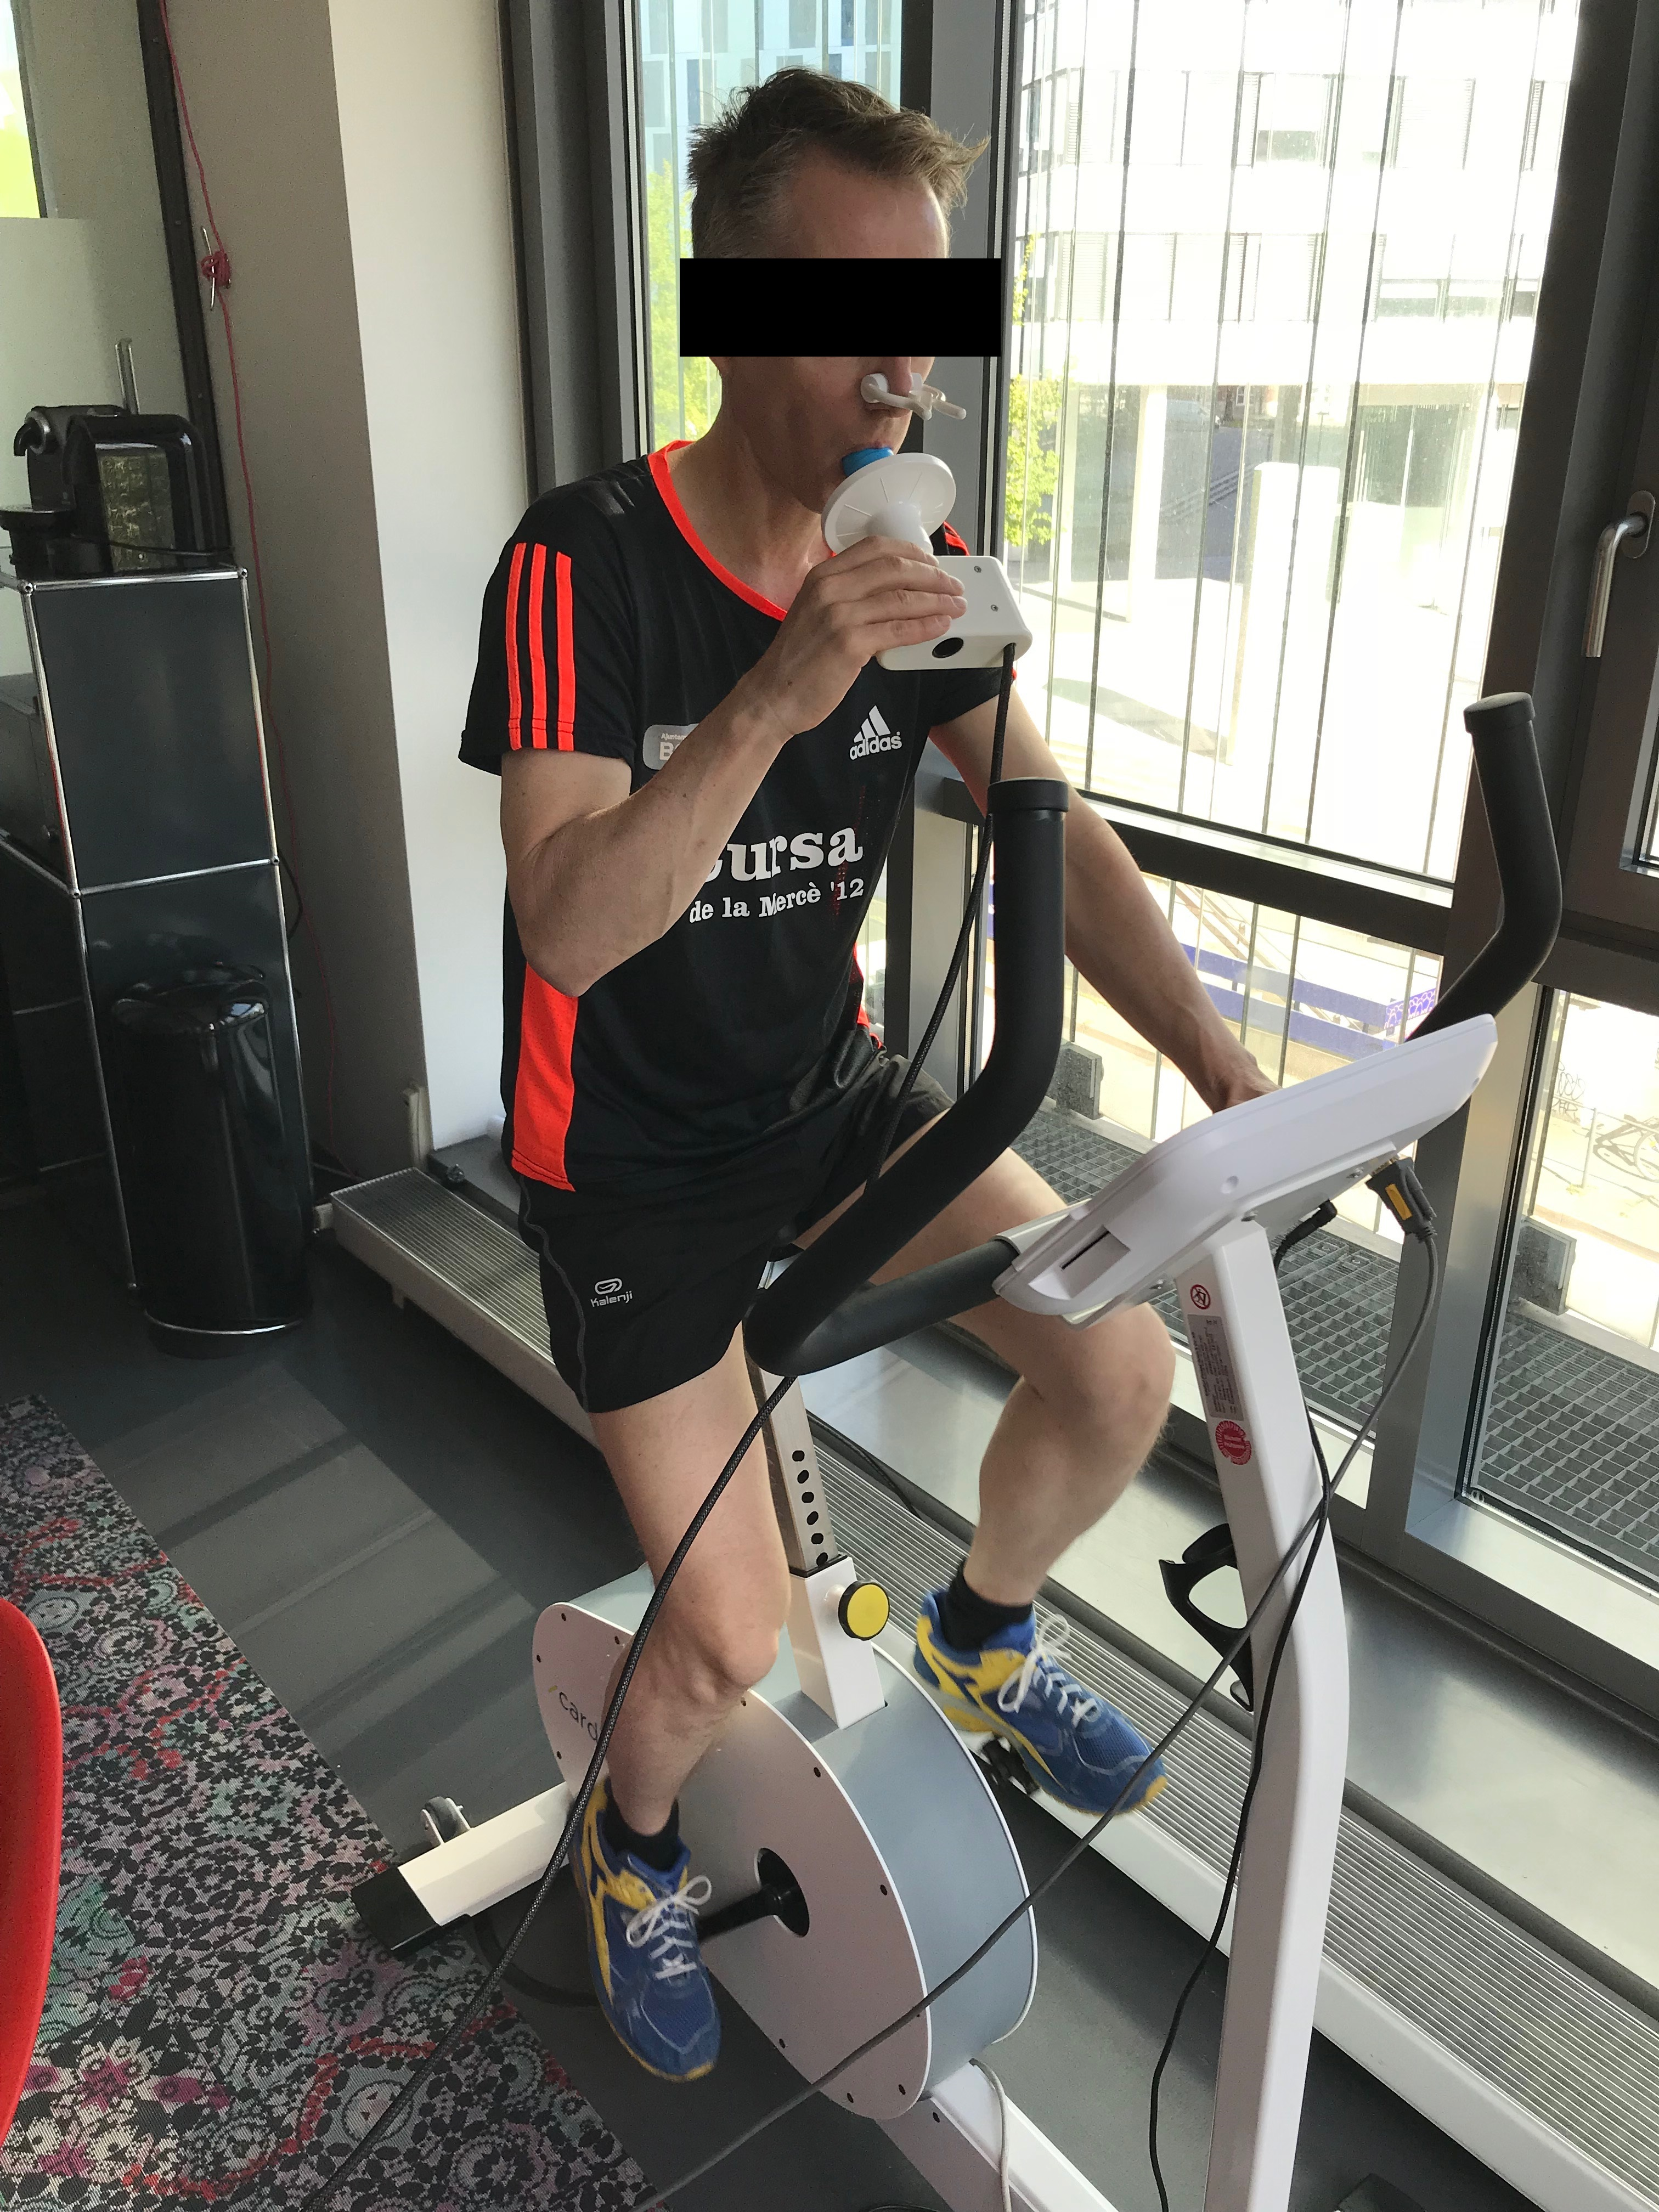
\includegraphics[width=90mm]{Bilder/proband.jpg}
	\caption{Proband während der Spiroergometrie}
	\label{pic:pic11}
\end{figure}

Abb. \ref{pic:pic11} zeigt beispielhaft eine Messung mit einem männlichen Probanden. Darauf zu erkennen sind das verwendete Fahrradergometer, das Atemmodul, der Filter, das Mundstück und die Nasenklammer. Grundsätzlich war es den Probanden freigestellt, ob sie das Mundstück mit der Hand halten oder mit dem Kiefer. Eventuelle Auswirkungen des Handlings auf die Durchführung oder Ergebnisse werden in dieser Arbeit nicht behandelt.\\
In Abb. \ref{pic:pic12} ist die Oberfläche der \acs{CCPS} zu sehen, wie sie während einer Spiroergometrie auf dem Laptop dargestellt ist. Der Bildausschnitt zeigt die Graphen und Messwerte sowie den besagten Timer (oben in schwarzer Schrift) innerhalb eines Interfaces. Der obere rechte Plot zeigt die aktuell gemessene Durchflussrate des Flowsensors. Ist diese >0, handelt es sich um eine Exspiration. Bei Werten <0 ist die Inspiration betroffen.

\begin{figure}[H]
	\centering
	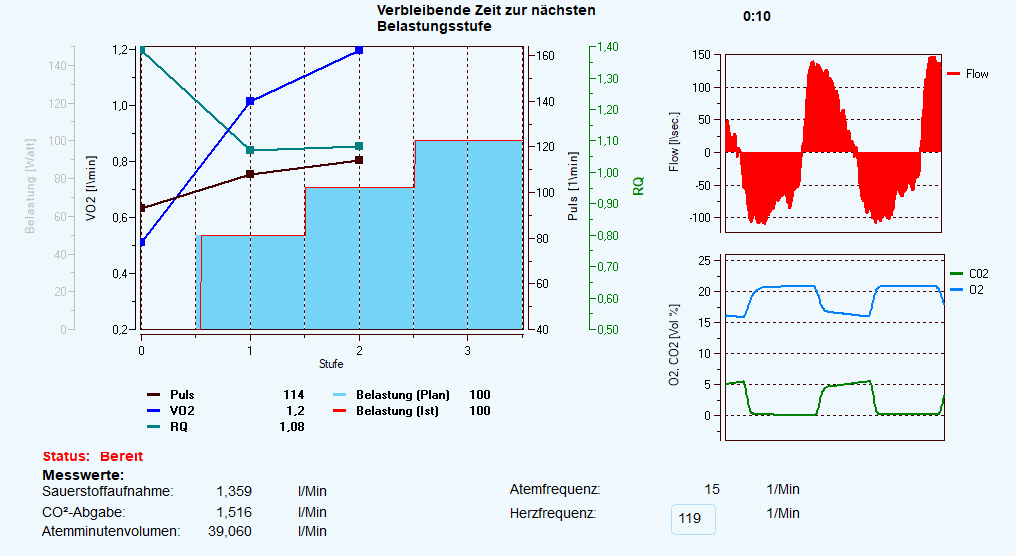
\includegraphics[width=\textwidth]{Bilder/sw_screen.png}
	\caption[Software-Oberfläche während einer Spiroergometrie]{Beispielhafte Darstellung der \acs{CCPS}-Oberfläche während einer Spiroergometrie}
	\label{pic:pic12}
\end{figure}

Unten rechts ist mit drei Sekunden Latenz ein Plot mit den \acs{O2}- und \acs{CO2}-Konzentrationen eines Atemzugs eingebunden. Der blaue Graph stellt die \acs{O2}-, der grüne die \acs{CO2}-Konzentration dar. Das große Fenster links oben bildet eine Verlaufsdarstellung bestimmter Parameter ab, die innerhalb einer Stufe gemittelt wurden. Anhand der X-Achse des Koordinatensystems sind Stufennummerierungen zu erkennen. Die Y-Achse ist mehrfach definiert und unterschiedlich skaliert. Dargestellt werden in verschiedenen Farben die pro Stufe ermittelten Durchschnittswerte für die \acs{VO2} (blau), den Puls bzw. die \acs{HF} (braun) und den \acs{RQ} (türkis) in Form eines Graphen sowie die während einer Stufe eingestellten Belastungsintensitäten als Balkendiagramm (hellblau). Durch einen roten Graphen wird auch die Steigerung der Intensität zu Stufenbeginn mit einem zeitlichen Bezug angedeutet. Unterhalb des Plots werden die Durchschnittswerte für besagte Parameter visualisiert, die bei der zuletzt abgeschlossenen Stufe durch die Software ausgewertet wurden. Außerdem werden im unteren Abschnitt des hellblauen Interfaces die während des letzten erkannten Atemzugs berechneten Werte für die \ac{VO2}, \ac{VCO2}, das \ac{AMV} und die \ac{AF} mitgeschrieben. Außerdem wird die vom Pulsgurt, via Ergometer an die Software übermittelte \ac{HF} angezeigt. Mithilfe dieses Interfaces konnte der Verlauf der Spiroergometrie überwacht und verfolgt werden. Der Timer half bei der korrekten Durchführung der Atemzugerfassung und die Graphen gaben Aufschluss darüber, ob diese korrekt funktionierte. Die Rohdaten der Sensoren wurden im Hintergrund aufgezeichnet, in \acs{CSV}-Dateien abgespeichert und konnten anschließend mit MATLAB ausgewertet werden.

\section{Datenverarbeitung \& Generierung der Plots}

\begin{figure}[H]
	\centering
	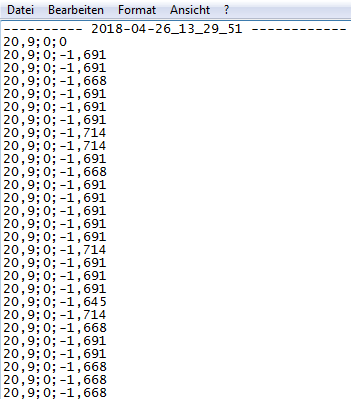
\includegraphics[width=55mm]{Bilder/breathdata.png}
	\caption[Rohdaten des metabolicscan]{Bildausschnitt einer Beispiel-CSV-Datei mit Rohdaten des metabolicscan}
	\label{pic:pic14}
\end{figure}

In Abb. \ref{pic:pic14} ist ein Ausschnitt des Anfangs einer CSV-Textdatei zu sehen, die nach Abschluss einer Messung durch die \acs{CCPS} gespeichert wurde. Die Messwerte des \acs{O2}-, \acs{CO2}- und Flowsensors werden von links nach rechts in drei durch Semikolons getrennten Spalten gespeichert. Die Datenmenge war je nach Gesamtdauer einer Leistungsdiagnostik unterschiedlich groß und manche Dateien bestanden aus Zeilen im fünfstelligen Bereich. Durch ein MATLAB-Skript wurden die Sensor-Rohdaten eingelesen und zur weiteren Verarbeitung vorbereitet. Anschließend durchliefen die Daten ein Unterprogramm, mit denen die einzelnen Atemzüge anhand des Flows identifiziert wurden. Das Ventilationsmuster eines Menschen ist allerdings sehr individuell und enthält häufig Artefakte, beispielsweise wenn die Atmung beim Schluckreflex unterbrochen wird. Rechen-Filter sorgten deshalb dafür, dass ein Flow-Intervall erst dann als ein neuer Atemzug gespeichert wurde, wenn bestimmte Schwellwerte überschritten wurden. Weitere Funktionen dienten der Zuordnung der entsprechenden \acs{O2}- und \acs{CO2}-Werte zu einem Atemzug, da die Sensoren diese erst nach ca. drei Sekunden Verzögerung liefern. Mit diesen Atemzugwerten wurde anschließend ein Mittelwert für jede bewältigte Belastungsstufe `{a} \SI{2}{\minute} berechnet. Die Mittelwerte wurden anschließend in mehreren Bezugssystemen grafisch aufgetragen. Am Ende der Ausführung des MATLAB-Skriptes wurden die Graphen für V-Slope, \acs{EQO2}/\acs{EQCO2}, \acs{VE}/\acs{VCO2}, \acs{RQ}, \acs{VE}/\acs{W} und \acs{VO2}/\acs{W} sowie eine übersichtliche und vereinfachte 6-Felder-Grafik als Bild-Dateien gespeichert. 

\section{Auswertung \& Referenzierung der Ergebnisse}

Schlussendlich wurden alle Plots zunächst subjektiv ausgewertet und die ventilatorischen Schwellen händisch bestimmt. Dabei wurden die Grafiken auf in Kapitel 1.2.2 genannte Indikatoren für die Schwellen analysiert. Da in der klinischen Spiroergometrie zumeist nach dem Mehr-Augen-Prinzip ausgewertet wird, analysierte unabhängig eine zweite Person die Ergebnisse, deren Ansichten in dieser Arbeit als Referenz dienen. Da cardioscan die Schwellenbestimmung auch in Zukunft automatisiert durch die Software durchführen lassen möchte, wurde das MATLAB-Programm durch Algorithmen für die automatische Auswertung der Graphen erweitert und als dritte Instanz hinzugefügt. Als Referenz für die Ergebnisse der Software dienten die Erkenntnisse der HUNT 3 Fitnessstudie von Loe et al. aus dem Jahre 2014~\cite{Loe.2014}. Im Zuge einer algorithmischen Schwellenbestimmung wurden die Ergebnisse durch die Software mit diesen Daten verglichen und auf Plausibilität überprüft. Die HUNT 3 Studie wurde zwar auf Laufbändern durchgeführt und beide Schwellen wurden ausschließlich mit der V-Slope-Methode bestimmt, jedoch bestand sie aus einer breit gefächerten Teilnehmergruppe mit 4631 Probanden. Daher bezeichnen Loe et al. ihre Erkenntnisse als größte europäische Referenzdaten-Sammlung für kardiorespiratorische Werte bei gesunden Männern und Frauen. Die Ergebnisse galt es anschließend zu vergleichen und auf Übereinstimmungen bzw. Differenzen zu analysieren.

\section{Probandendaten}

Tab. \ref{tab:tabelle3} listet die Probanden-Daten Geschlecht, Gewicht in \si{\kilogram}, Körpergröße in \si{\centi\metre}, Alter in Lebensjahren, sportliche Aktivität in \si{\hour} pro Woche und die eigene Aussage, ob man Raucher ist oder nicht, auf. Unter den 28 Probanden waren zwölf Frauen und 16 Männer sowie fünf Raucher. Das Gesamtdurchschnittsalter betrug 33 Jahre. Das durchschnittliche Alter der Männer lag bei 35, das der Frauen bei 29 Jahren. Unter den Testpersonen befanden sich fünf Leistungssportler, von denen einer Olympionik ist. Im Mittel lag die wöchentliche sportliche Aktivität der Männer bei sieben, die der Frauen bei sechs Stunden. Anzumerken ist, dass es sich bei diesen Zahlen um subjektive Einschätzungen der Personen handelt und eventuell nicht die realen Gegebenheiten widerspiegeln. Dies liegt daran, dass "`sportliche Aktivität"' nicht eindeutig definiert ist und einige Probanden keine festen Trainingszeiten besitzen und daher unregelmäßig zum Sport gehen. Die Angaben wurden genutzt, um das Belastungsprotokoll, wie in Kapitel 2.2.1 beschrieben, anzupassen.

\begin{table}[H]
	\centering
	\caption{Daten und Eigenschaften der getesteten Probanden}
	\medskip
	\begin{tabulary}{\textwidth}{L C C C C C C}
		\toprule
		ID & Geschlecht & Gewicht in \si{\kilogram} & Größe in \si{\centi\metre} & Alter & Raucher & Akt. in \si{\hour\per Woche} \\
		\midrule
		\midrule
		1w & w & 65 & 171 & 40 & nein & 3,5 \\
		2w & w & 66 & 166 & 21 & ja & 2,5 \\
		3w & w & 70 & 163 & 31 & nein & 18 \\
		4m & m & 71 & 174 & 48 & nein & 5,5 \\
		5w & w & 56 & 167 & 25 & nein & 2 \\
		6w & w & 75 & 168 & 45 & ja & 6 \\
		7m & m & 86 & 178 & 37 & nein & 3 \\
		8m & m & 79 & 185 & 29 & nein & 13 \\
		9m & m & 94 & 178 & 44 & nein & 4 \\
		10w & w & 64 & 161 & 28 & nein & 11,5 \\
		11m & m & 75 & 176 & 26 & nein & 4 \\
		12m & m & 71 & 181 & 32 & nein & 6 \\
		13m & m & 93 & 171 & 29 & nein & 8 \\
		14m & m & 84 & 181 & 25 & nein & 35 \\
		15m & m & 97 & 187 & 28 & nein & 8 \\
		16w & w & 81 & 169 & 28 & ja & 1,5 \\
		17w & w & 49 & 155 & 20 & nein & 9 \\
		18w & w & 67 & 172 & 19 & nein & 8 \\
		19w & w & 50 & 156 & 47 & nein & 2 \\
		20m & m & 63 & 178 & 21 & ja & 2 \\
		21m & m & 105 & 184 & 21 & nein & 2 \\
		22m & m & 85 & 171 & 43 & ja & 0 \\
		23w & w & 64 & 174 & 40 & nein & 6 \\
		24m & m & 72 & 173 & 49 & nein & 5 \\
		25m & m & 68 & 174 & 58 & nein & 5 \\
		26m & m & 76 & 183 & 34 & nein & 7,5 \\
		27m & m & 101 & 192 & 34 & nein & 5 \\
		28w & w & 69 & 169 & 33 & nein & 3 \\
		\bottomrule
	\end{tabulary}
	\label{tab:tabelle3}
\end{table}
	\chapter{Resultate}
%
Zu Beginn dieses Kapitels werden einige Plots präsentiert, die für die Auswertung verwendet wurden. Anschließend werden Unterschiede zwischen den Ergebnissen aufgezeigt, die im nächsten Kapitel für die Evaluierung der Methoden diskutiert werden. Alle Messungen wurden ohne Störungen oder Fehler von außerhalb erfolgreich durchgeführt.\\
Die nachfolgende Tab. \ref{tab:tabelle4} zeigt zu jeder Testperson die vorab ermittelte Ruhe-\gls{HF}, die während der Leistungsdiagnostik \gls{HFmax} sowie die \gls{Wstart}, die \gls{Wmax} und die \acrfull{VO2max}. 16 von 28 Personen mussten die Belastungsphase laut eigener Aussage wegen Beinschwäche beenden. Zehn Probanden erreichten nach Selbsteinschätzung ihr konditionales Maximum. Zwei Personen klagten in der letzten Stufe über Atemnot und mussten den Test deshalb abbrechen.
%
\begin{table}[H]
	\centering
		\caption{Originäre Messergebnisse der Tests}
		\medskip
		\begin{tabulary}{\textwidth}{L C C C C C}
			\toprule
			ID & Ruhe-\gls{HF} in \si{\per\minute} & \gls{HFmax} in \si{\per\minute} & \gls{Wstart} in \si{\watt} & \gls{Wmax} in \si{\watt} & \gls{VO2max} in \si{\litre\per\minute} \\
			\midrule
			\midrule
			1w & 65 & 175 & 40 & 215 & 2,4 \\
			2w & 63 & 183 & 35 & 185 & 2,1 \\
			3w & 53 & 158 & 50 & 225 & 2,7 \\
			4m & 49 & 164 & 50 & 300 & 3,6 \\
			5w & 85 & 187 & 40 & 165 & 2,15 \\
			6w & 65 & 178 & 30 & 205 & 2,55 \\
			7m & 78 & 176 & 55 & 280 & 3,3 \\
			8m & 76 & 195 & 90 & 315 & 4 \\
			9m & 64 & 181 & 40 & 340 & 4,05 \\
			10w & 62 & 168 & 40 & 215 & 2,78 \\
			11m & 90 & 178 & 40 & 215 & 2,6 \\
			12m & 61 & 180 & 75 & 325 & 4 \\
			13m & 62 & 176 & 75 & 275 & 3,45 \\
			14m & 63 & 179 & 100 & 325 & 3,85 \\
			15m & 87 & 193 & 80 & 330 & 4,05 \\
			16w & 84 & 198 & 40 & 240 & 2,98 \\
			17w & 78 & 194 & 50 & 175 & 2 \\
			18w & 68 & 182 & 50 & 225 & 2,7 \\
			19w & 66 & 172 & 40 & 165 & 2,13 \\
			20m & 68 & 197 & 60 & 210 & 2,83 \\
			21m & 92 & 195 & 50 & 275 & 3,4 \\
			22m & 72 & 159 & 50 & 225 & 3,05 \\
			23w & 67 & 173 & 40 & 265 & 3,18 \\
			24m & 94 & 174 & 50 & 250 & 2,83 \\
			25m & 62 & 167 & 50 & 250 & 3,15 \\
			26m & 77 & 169 & 60 & 285 & 3,5 \\
			27m & 86 & 193 & 60 & 285 & 3,58 \\
			28w & 78 & 220 & 40 & 190 & 2,5 \\
			\bottomrule
		\end{tabulary}
		\label{tab:tabelle4}
\end{table}
%
\section{Grafiken zur Bestimmung der Schwellen}
%
\subsection{Manuelle Bestimmung}
%
\begin{figure}[H]
	\centering
	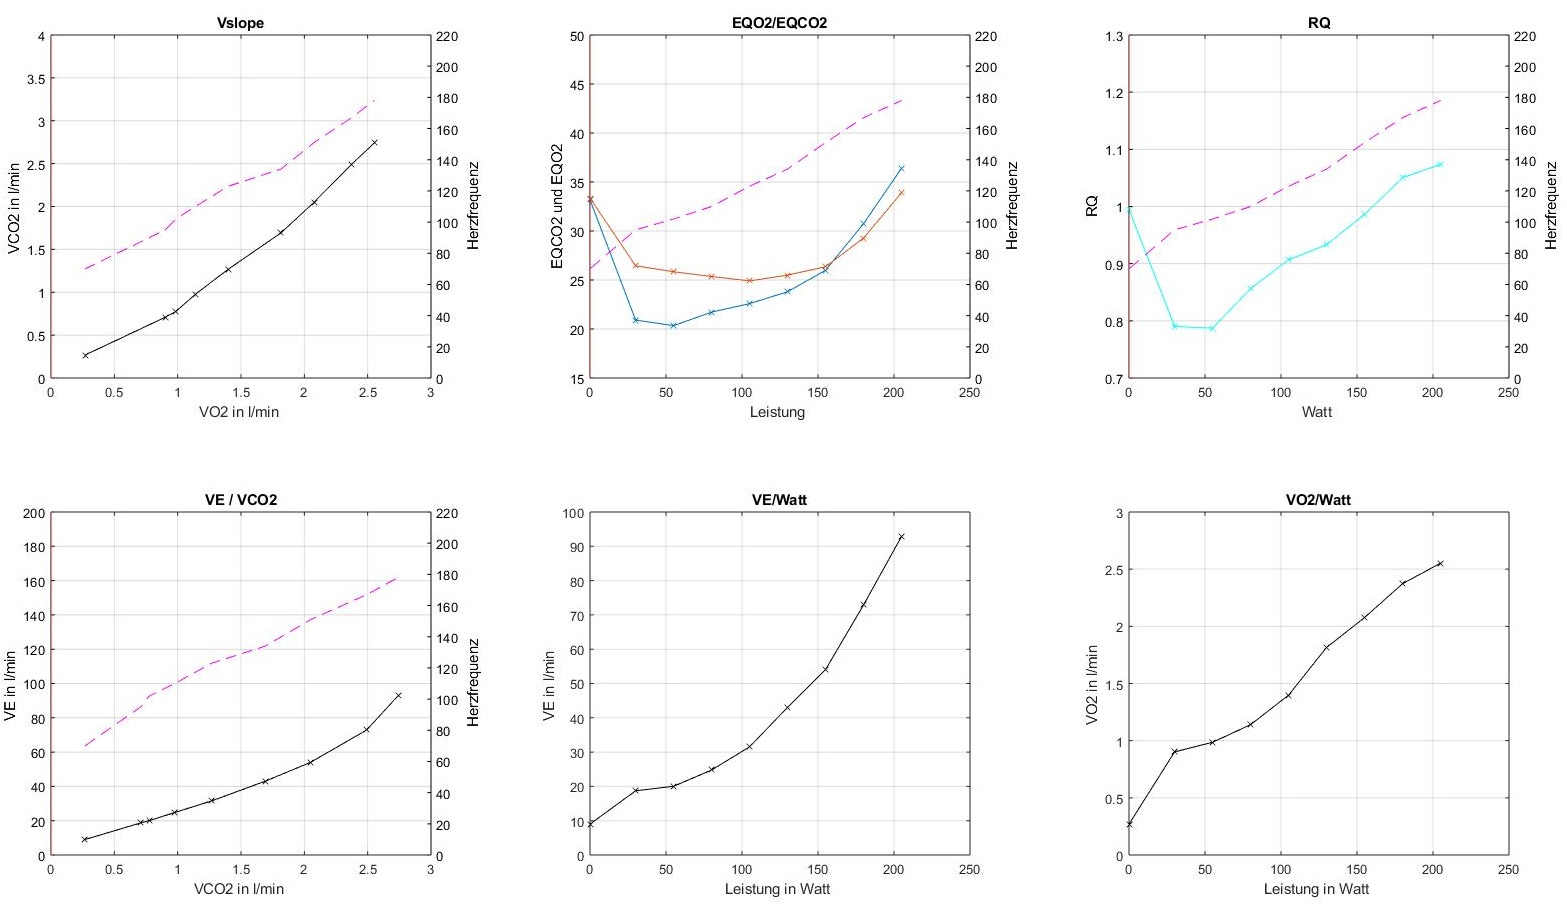
\includegraphics[width=\textwidth]{Bilder/plot_6w.jpg}
	\caption[6-Felder-Grafik von Probandin 6w]{6-Felder-Grafik von Probandin 6w; Feld 1: \gls{VCO2} in \si{\litre\per\minute} gegenüber der \gls{VO2} in \si{\litre\per\minute}; Feld 2: \gls{EQO2} in blau und \gls{EQCO2} in orange gegenüber der Leistung in \si{\watt}; Feld 3: \gls{RQ} gegenüber der Leistung in \si{\watt}; Feld 4: \gls{VE} in \si{\litre\per\minute} gegenüber der \gls{VCO2} in \si{\litre\per\minute}; Feld 5: \gls{VE} in \si{\litre\per\minute} gegenüber der Leistung in \si{\watt}; Feld 6: \gls{VO2} in \si{\litre\per\minute} gegenüber der Leistung in \si{\watt}; rosa gestrichelte Linie in Feld 1-4: \gls{HF} in \si{\per\minute}}
	\label{pic:pic15}
\end{figure}
%
Beginnend mit Abb. \ref{pic:pic15} für Probandin 6w werden beispielhaft Grafiken verschiedener Probanden vorgestellt, anhand derer die ventilatorischen Schwellen von den menschlichen Ratern subjektiv bestimmt wurden. Sie bestehen insgesamt aus sechs Feldern. Die ersten vier Felder stellen jeweils eine Methode zur Bestimmung der Schwellen dar. Sie enthalten zur erleichterten optischen Auswertung den Verlauf der \gls{HF} als rosafarbenen gestrichelten Graphen. Je nach Skalierung der Achsen, nimmt diese unterschiedliche Formen an und dient nur zum Vergleich mit den Graphen in demselben Feld. Sie wird durch die rechte Y-Achse skaliert. In Feld 5 und 6 werden die \gls{VE} sowie \gls{VO2} mit der Leistung (hier als "`Watt"' bezeichnet) in Relation gesetzt. Diese Plots wurden erstellt, um den Messungserfolg evaluieren zu können. Die Kreuze in den Kurven stellen die Mittelwerte einer Stufe dar und spiegeln in ihrer Menge die Anzahl der gefahrenen Belastungsstufen wider.
%
\begin{figure}[H]
	\centering
	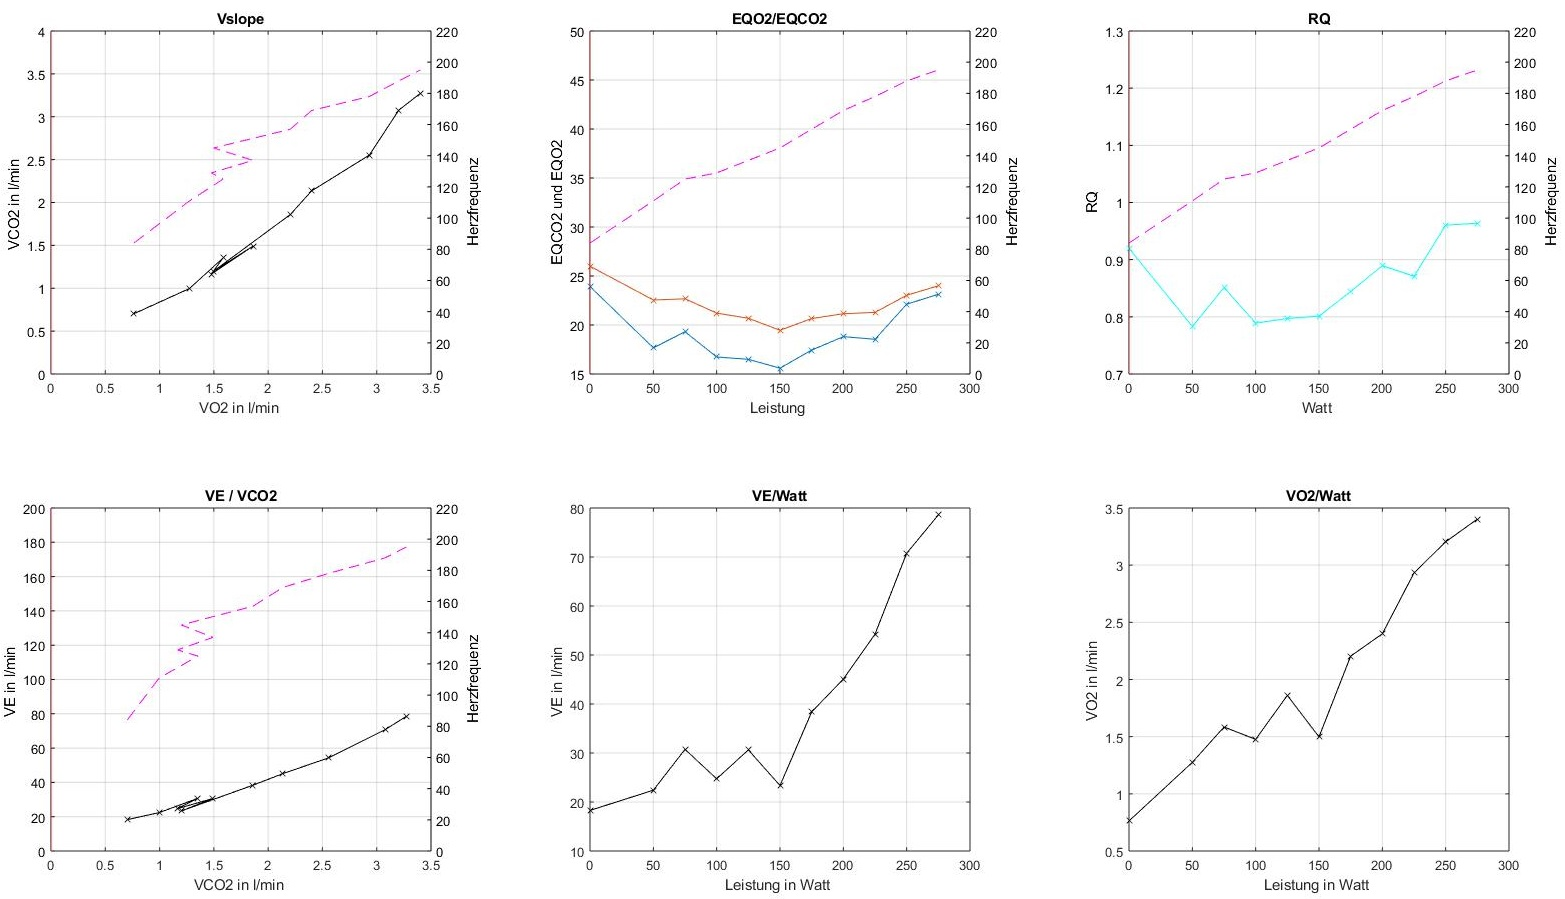
\includegraphics[width=\textwidth]{Bilder/plot_21m.jpg}
	\caption[6-Felder-Grafik von Proband 21m]{6-Felder-Grafik von Proband 21m; Feld 1: \gls{VCO2} in \si{\litre\per\minute} gegenüber der \gls{VO2} in \si{\litre\per\minute}; Feld 2: \gls{EQO2} in blau und \gls{EQCO2} in orange gegenüber der Leistung in \si{\watt}; Feld 3: \gls{RQ} gegenüber der Leistung in \si{\watt}; Feld 4: \gls{VE} in \si{\litre\per\minute} gegenüber der \gls{VCO2} in \si{\litre\per\minute}; Feld 5: \gls{VE} in \si{\litre\per\minute} gegenüber der Leistung in \si{\watt}; Feld 6: \gls{VO2} in \si{\litre\per\minute} gegenüber der Leistung in \si{\watt}; rosa gestrichelte Linie in Feld 1-4: \gls{HF} in \si{\per\minute}}
	\label{pic:pic16}
\end{figure}
%
Abb. \ref{pic:pic16} zeigt eine weitere 6-Felder-Grafik von Proband 21m. Diese beinhaltet unregelmäßige Graphen und es ist zu sehen, dass der RQ (hellblau) während des Tests den Wert eins nicht überschritten hat. Außerdem tritt in der \gls{EQCO2}-Kurve kein signifikanter Anstieg zum Ende der Leistungsdiagnostik auf. Die Graphen im 5. und 6. Feld besitzen in Abb. \ref{pic:pic15} stetige Steigungen. In Abb. \ref{pic:pic16} schwanken die Kurven zwischen einzelnen Messpunkten. Die übrigen Plots weisen an den betroffenen Stufen Analogien zu diesen Schwankungen auf. In Kapitel 4 werden diese Eigenschaften genauer erörtert.
%
\subsection{Algorithmische Bestimmung}
%
In diesem Abschnitt werden weitere Grafiken präsentiert, die zusätzlich eine algorithmische Schwellenbestimmung des MATLAB-Programms enthalten. Hierdurch wurde für jeden Probanden eine zweite Bilddatei erstellt, welche die VT1 und VT2 bereits in Form von vertikalen Linien beinhaltet und durch eine Angabe für die \gls{HF} an der jeweiligen Schwelle ergänzt ist. In Feld 5 dieser Plots wurde im Vergleich mit der \gls{VE} die Leistung durch die \gls{HF} ersetzt und es wurden bereits Trainingsbereiche eingefügt, die ebenfalls durch farbige vertikale Linien gekennzeichnet und in einer Legende mit Wertebereichen beschrieben sind. Es werden \gls{REKOM}, \gls{GA1}, \gls{GA2}, \gls{EW} und Leistung als Trainingszonen definiert. Dies diente dem Testlauf eines neuen Modells zur Trainingssteuerung. Die Entwicklung und Implementierung dieses Modells basierte auf den Erkenntnissen zur Schwellenbestimmung und wurde nachträglich eingefügt. Im Kapitel 5 wird näher darauf eingegangen.
%
\begin{figure}[H]
	\centering
	\noindent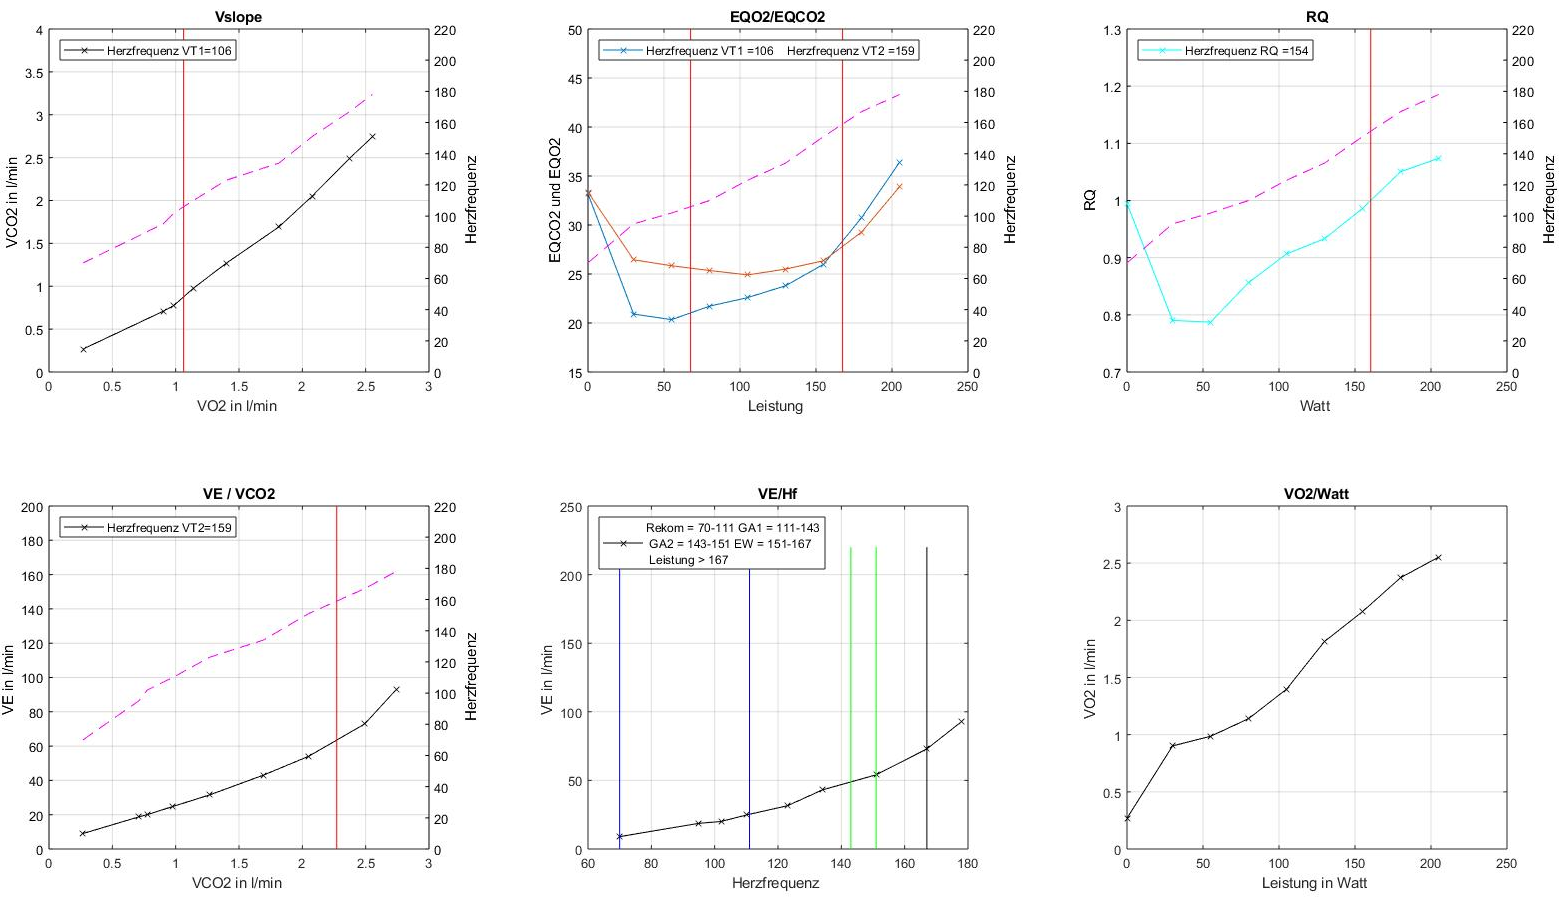
\includegraphics[angle=0,width=\linewidth,keepaspectratio]{Bilder/auto_6}
	\caption[6-Felder-Grafik von Probandin 6w mit algorithmischen Schwellenmarkierungen]{6-Felder-Grafik von Probandin 6w mit algorithmischen Schwellenmarkierungen in Form vertikaler roter Linien: \textsl{V-Slope} = \SI{106}{\per\minute}, \textsl{\gls{EQO2}} = \SI{106}{\per\minute}, \textsl{\gls{EQCO2}} = \SI{159}{\per\minute}, \textsl{\gls{VE}/\gls{VCO2}} = \SI{159}{\per\minute}\\Feld 5: \gls{VE} in \si{\litre\per\minute} gegenüber der \gls{HF} in \si{\per\minute} mit eingefügten Trainingszonen \gls{REKOM}, \gls{GA1}, \gls{GA2}, \gls{EW} und Leistung, abgegrenzt durch vertikale farbige Linien}
	\label{pic:pic17}
\end{figure}
%
Die Plots in Abb. \ref{pic:pic17} zeigen die detektierten Schwellen für Probandin 6w nach acht Stufen, bei der jeweils beide Methoden für die VT1 sowie VT2 identische Ergebnisse brachten. Im blauen \gls{EQO2}-Graphen ist zu sehen, dass VT1 zwischen Tiefpunkt und darauffolgendem Messpunkt bestimmt wurde. Am \gls{EQCO2} ist erkennbar, dass die VT2 beim ersten signifikanten Kurvenanstieg markiert wurde. Bei der Probandin stieg in der 7. Stufe der RQ über eins hinaus. Die mithilfe dieser Methode erhobene VT2 liegt bei einer \gls{HF} von \SI{154}{\per\minute}.
%
\begin{figure}[H]
	\centering
	\noindent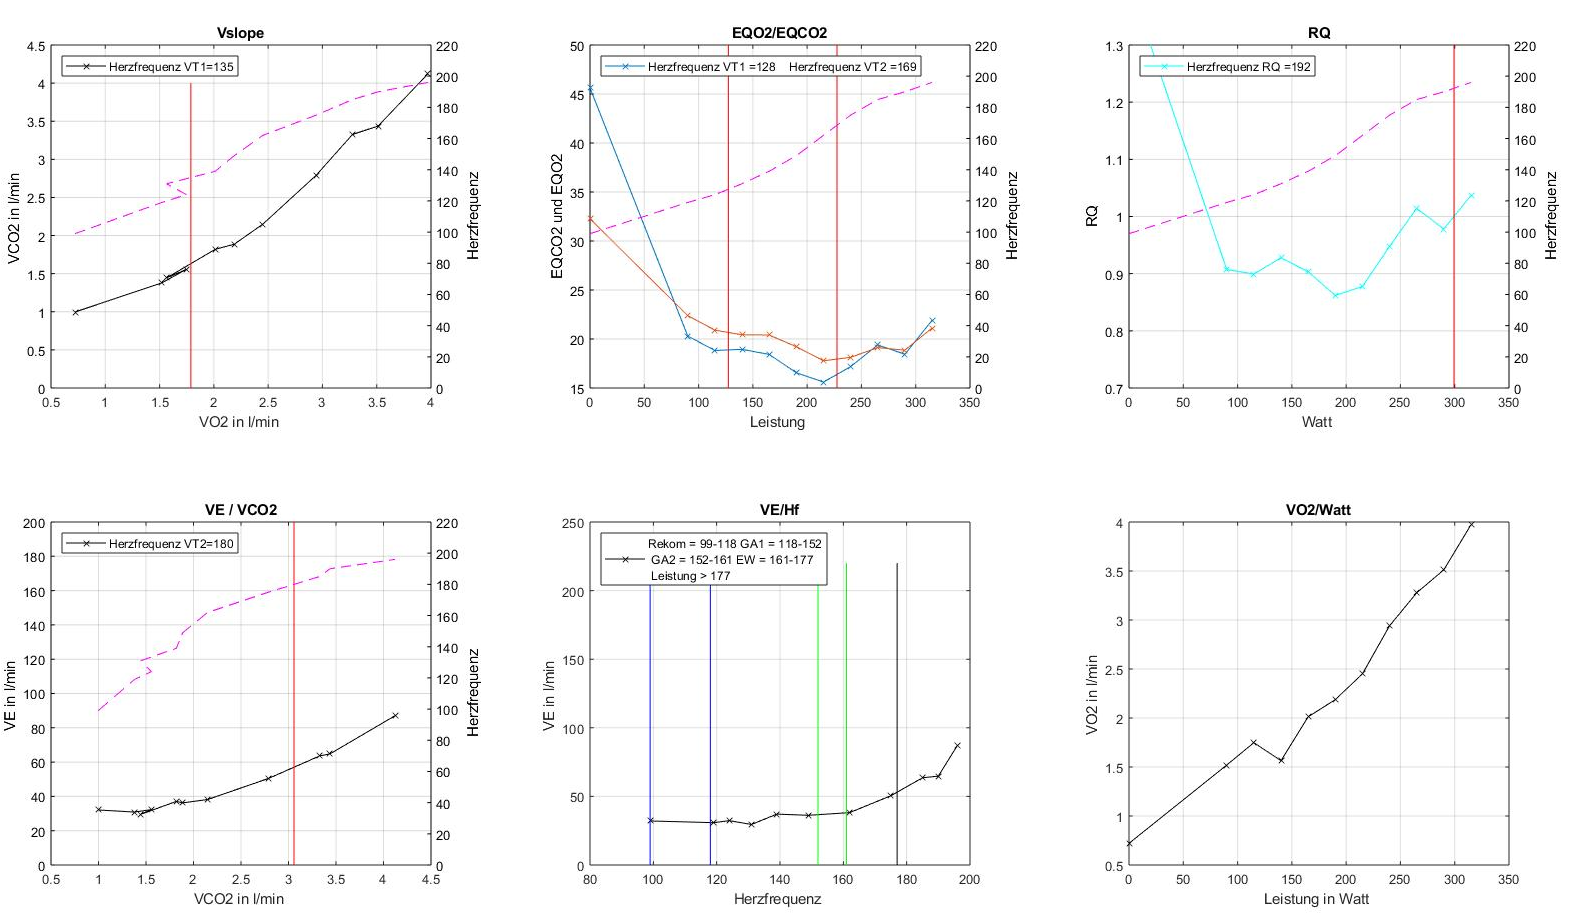
\includegraphics[angle=0,width=\linewidth,keepaspectratio]{Bilder/auto_8}
	\caption[6-Felder-Grafik von Proband 8m mit algorithmischen Schwellenmarkierungen]{6-Felder-Grafik von Proband 8m mit algorithmischen Schwellenmarkierungen: \textsl{V-Slope} = \SI{135}{\per\minute}, \textsl{\gls{EQO2}} = \SI{126}{\per\minute}, \textsl{\gls{EQCO2}} = \SI{169}{\per\minute}, \textsl{\gls{VE}/\gls{VCO2}} = \SI{180}{\per\minute}}
	\label{pic:pic18}
\end{figure}
%
In Abb. \ref{pic:pic18} ist die Grafik für Proband 8m erkennbar. Die \gls{HF} und der V-Slope in Feld 1 sowie \gls{VE}/\gls{VCO2} in Feld 4 sind zwischen Stufe 2 und 4 nicht differenzierbar. Die \gls{VO2} fällt im 6. Feld zwischen diesen Stufen. Der RQ schwankt zwischen den letzten zwei Messungen um den Wert eins herum und die Software bestimmte den zweiten Anstieg über eins bei \SI{192}{\per\minute} als VT2.\\
Abb. \ref{pic:pic19} stellt das Ergebnis von Proband 9m dar, der sogar 13 Belastungsstufen bewältigte. Mit RQ~=~1 wurde in der letzten Stufe bei \SI{173}{\per\minute} die VT2 markiert. In Feld 5 und 6 sind Schwankungen im Anstieg der \gls{VE} und \gls{VO2} in Relation zur \gls{HF} bzw. Belastung erkennbar.
%
\begin{figure}[H]
	\centering
	\noindent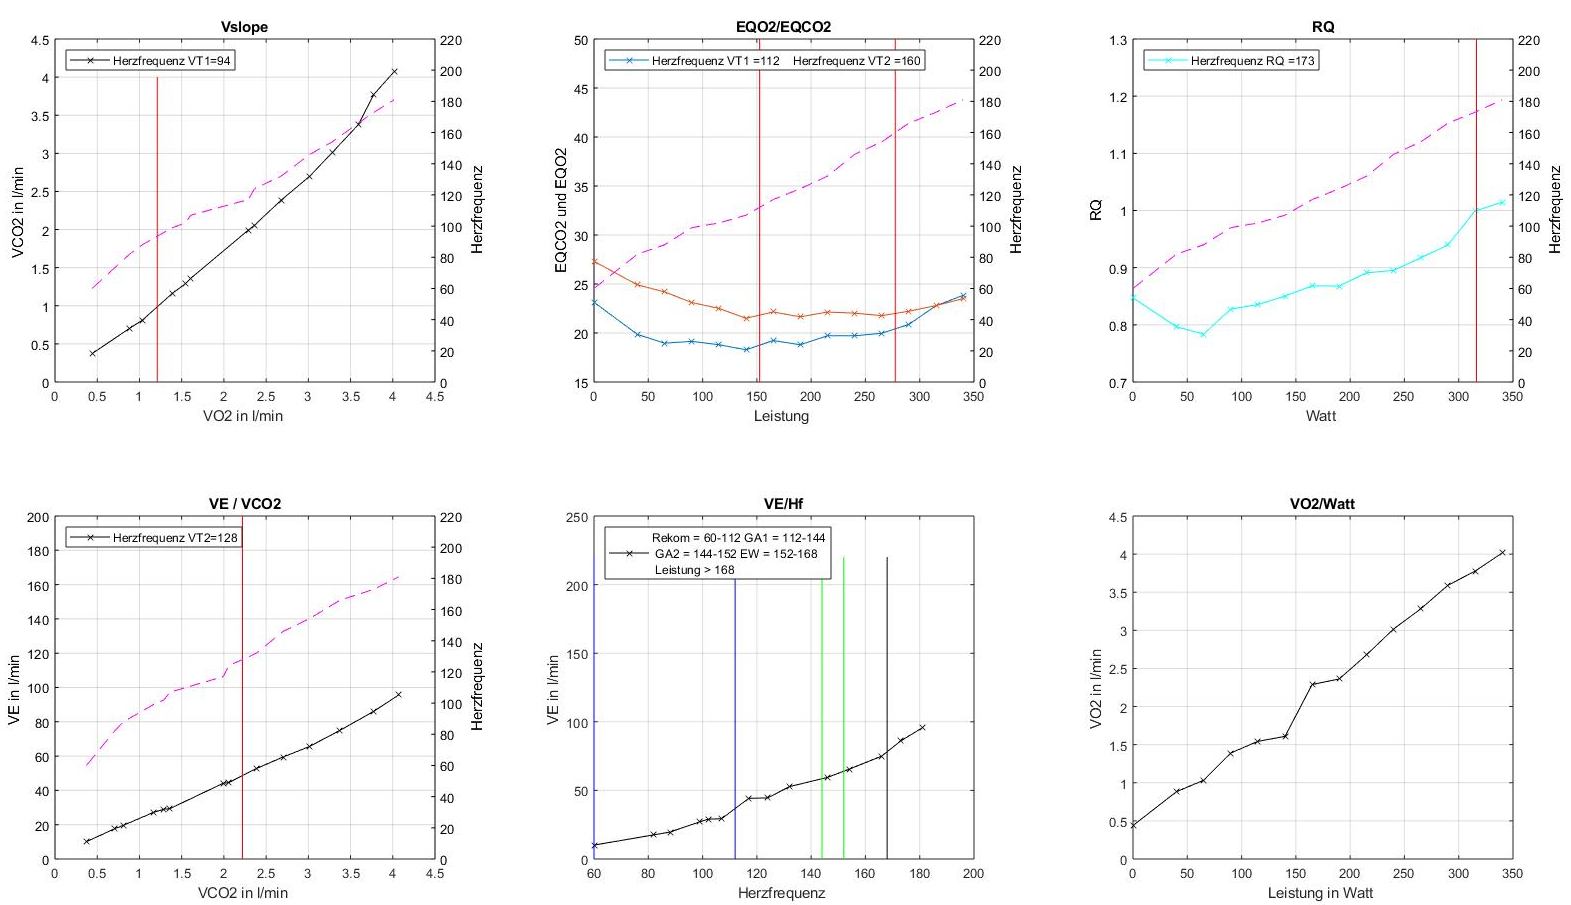
\includegraphics[angle=0,width=\linewidth,keepaspectratio]{Bilder/auto_9}
	\caption[6-Felder-Grafik von Proband 9m mit algorithmischen Schwellenmarkierungen]{6-Felder-Grafik von Proband 9m mit algorithmischen Schwellenmarkierungen: \textsl{V-Slope} = \SI{94}{\per\minute}, \textsl{\gls{EQO2}} = \SI{112}{\per\minute}, \textsl{\gls{EQCO2}} = \SI{160}{\per\minute}, \textsl{\gls{VE}/\gls{VCO2}} = \SI{128}{\per\minute}}
	\label{pic:pic19}
\end{figure}
%
\begin{figure}[H]
	\centering
	\noindent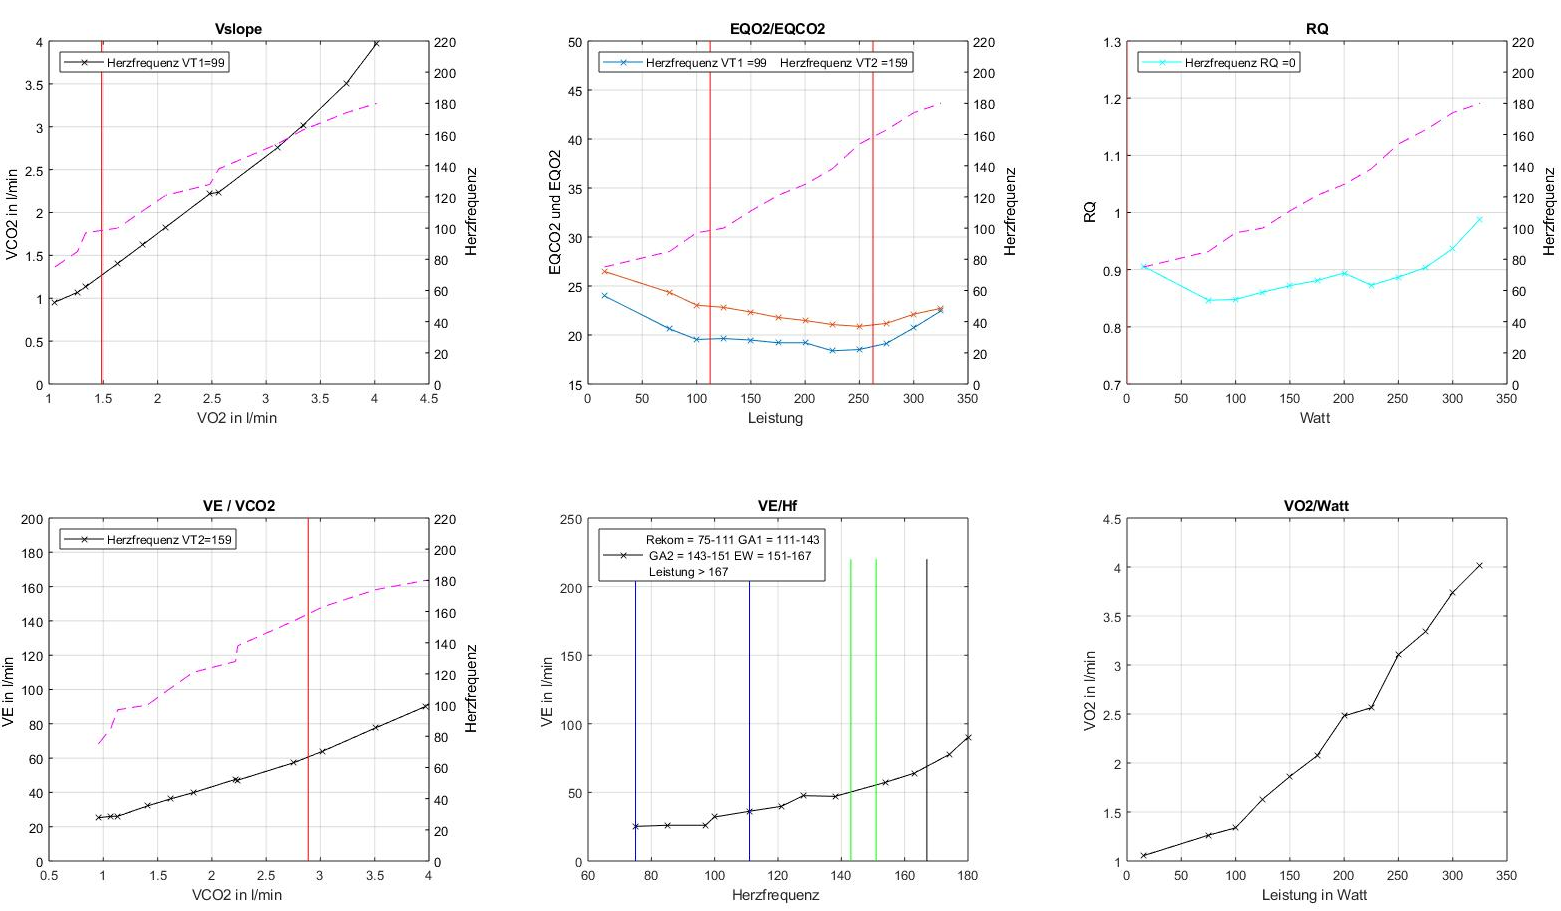
\includegraphics[angle=0,width=\linewidth,keepaspectratio]{Bilder/auto_12}
	\caption[6-Felder-Grafik von Proband 12m mit algorithmischen Schwellenmarkierungen]{6-Felder-Grafik von Proband 12m mit algorithmischen Schwellenmarkierungen: \textsl{V-Slope} = \SI{99}{\per\minute}, \textsl{\gls{EQO2}} = \SI{99}{\per\minute}, \textsl{\gls{EQCO2}} = \SI{159}{\per\minute}, \textsl{\gls{VE}/\gls{VCO2}} = \SI{159}{\per\minute}}
	\label{pic:pic20}
\end{figure}
%
In Abb. \ref{pic:pic20} ist eine Auswertung für Proband 12m zu sehen, welcher wiederum insgesamt elf Belastungsstufen absolvierte. Hier wurden die VT1 und VT2 ebenfalls mit beiden jeweiligen Methoden gleich bestimmt. Der RQ in Feld 3 stieg nicht über eins. Da die VT2 durch diese Methode vom Algorithmus nicht bestimmt werden konnte, ist der Wert null in der Legende angegeben. Im V-Slope sind mehrere Knickpunkte zu erkennen. Im 2. Feld tritt der Tiefpunkt des \gls{EQO2} erst in der 7. Stufe auf. Das \gls{EQCO2} sinkt an diesem Punkt noch, steigt jedoch ab der nächsten Stufe an. Im \gls{VO2}/Watt-Vergleich ist ein Knickpunkt mit geringerer Steigung ebenfalls nach der 7. Stufe zu sehen.
%
\begin{figure}[H]
	\centering
	\noindent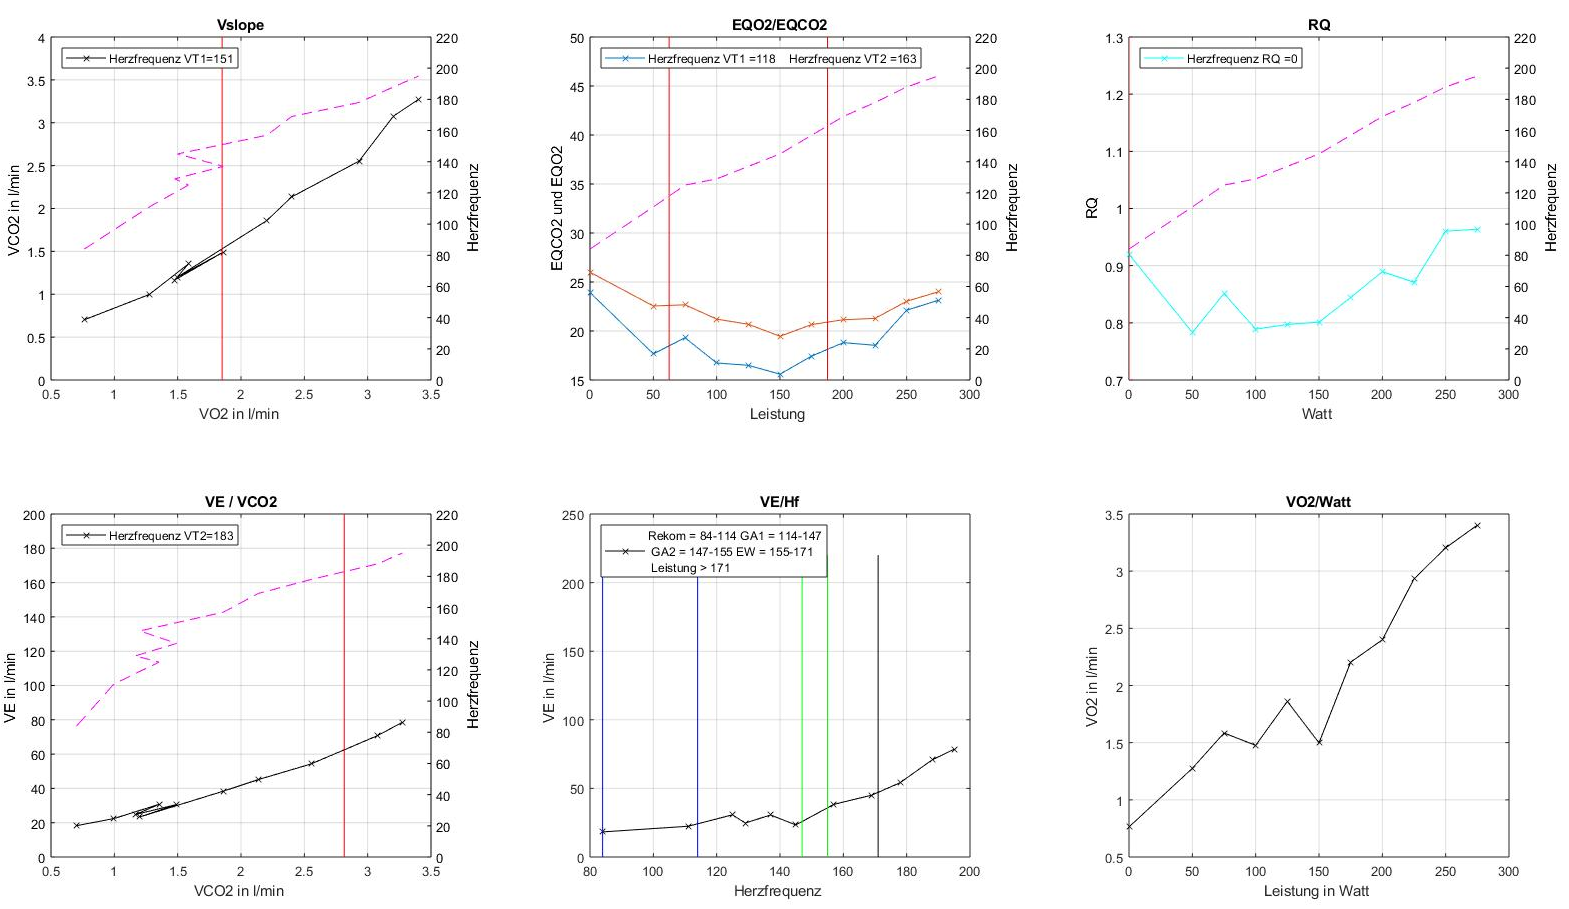
\includegraphics[angle=0,width=\linewidth,keepaspectratio]{Bilder/auto_21}
	\caption[6-Felder-Grafik von Proband 21m mit algorithmischen Schwellenmarkierungen]{6-Felder-Grafik von Proband 21m mit algorithmischen Schwellenmarkierungen: \textsl{V-Slope} = \SI{151}{\per\minute}, \textsl{\gls{EQO2}} = \SI{118}{\per\minute}, \textsl{\gls{EQCO2}} = \SI{163}{\per\minute}, \textsl{\gls{VE}/\gls{VCO2}} = \SI{183}{\per\minute}}
	\label{pic:pic21}
\end{figure}
%
Die vierte Beispielgrafik in Abb. \ref{pic:pic21} zeigt die Ergebnisse des Probanden 21m analog zu Abb. \ref{pic:pic16} inklusive der Schwellenbestimmung der Software. Dieser Proband bewältigte zehn Belastungsstufen. Im 6. Feld ist eine schwankende Steigung der \gls{VO2} in Relation zur Belastung zwischen Stufe 2 und 5 erkennbar. Diese Schwankungen tauchen auch im V-Slope und bei \gls{VE}/\gls{VCO2} sowie beim RQ auf. Auch hier unterscheiden sich die Bestimmungen für die VT1 durch den V-Slope und das \gls{EQO2} sowie jene für die VT2 anhand des \gls{EQCO2} oder \gls{VE}/\gls{VCO2}. Wie bereits in Abschnitt 3.3.1 erwähnt, erreichte der RQ dieses Probanden nicht den Wert eins.
%
\section{Ergebnisse der Schwellenbestimmung}
%
\subsection{Ergebnisse für die VT1}
%
\begin{table}[H]
	\begin{center}
		\caption{Ergebnisse für die \gls{HF} in \si{\per\minute} bei der VT1}
		\medskip
		\begin{tabulary}{\textwidth}{L@{\hspace{3em}} C C C C C C}
			\toprule
			& \multicolumn{2}{c}{\textbf{Rater 1}} & \multicolumn{2}{c}{\textbf{Rater 2}} & \multicolumn{2}{c}{\textbf{Software}} \\
			\midrule
			ID & V-Slope & \gls{EQO2} & V-Slope & \gls{EQO2} & V-Slope & \gls{EQO2} \\
			\midrule
			\midrule
			1w & 109 & 133 & 133 & 130 & 101 & 132 \\
			2w & 119 & 120 & 126 & 126 & 121 & 121 \\
			3w & 115 & 116 & 118 & 116 & 97 & 117 \\
			4m & 98 & 99 & 100 & 100 & 98 & 98 \\
			5w & 118 & 120 & 115 & 122 & 124 & 124 \\
			6w & 102 & 106 & 106 & 109 & 106 & 106 \\
			7m & 105 & 115 & 105 & 145 & 105 & 114 \\
			8m & 120 & 126 & 155 & 168 & 135 & 128 \\
			9m & 110 & 115 & 92 & 116 & 94 & 112 \\
			10w & 118 & 117 & 118 & 118 & 117 & 117 \\
			11m & 114 & 115 & 135 & 135 & 114 & 135 \\
			12m & 142 & 140 & 148 & 158 & 99 & 99 \\
			13m & 115 & 116 & 116 & 116 & 116 & 116 \\
			14m & 116 & 118 & 129 & 132 & 134 & 110 \\
			15m & 118 & 118 & 145 & 146 & 146 & 120 \\
			16w & 130 & 150 & 152 & 153 & 130 & 130 \\
			17w & 138 & 138 & 135 & 138 & 136 & 136 \\
			18w & 135 & 137 & 138 & 138 & 102 & 140 \\
			19w & 122 & 122 & 138 & 152 & 135 & 126 \\
			20m & 116 & 116 & 110 & 110 & 114 & 114 \\
			21m & 118 & 115 & 160 & 152 & 151 & 118 \\
			22m & 108 & 108 & 109 & 110 & 110 & 101 \\
			23w & 110 & 120 & 110 & 146 & 111 & 87 \\
			24m & 113 & 115 & 115 & 117 & 117 & 111 \\
			25m & 100 & 100 & 100 & 135 & 104 & 104 \\
			26m & 140 & 140 & 141 & 140 & 112 & 142 \\
			27m & 110 & 130 & 130 & 132 & 134 & 134 \\
			28w & 103 & 120 & 108 & 120 & 109 & 122 \\
			\bottomrule
		\end{tabulary}
		\label{tab:tabelle5}
	\end{center}
\end{table}
%
In Tab. \ref{tab:tabelle5} werden die Ergebnisse der VT1-Bestimmung der Rater und der Software für alle 28 Testpersonen verglichen. In sechs Spalten wird, geordnet nach Methode und Rater, die \gls{HF} aufgeführt, die an Stelle der VT1 abgelesen bzw. durch die Software bestimmt wurden. Es werden dabei auch nebeneinander die Methoden in direkte Relation gesetzt. Bei einigen Probanden sind zwischen den jeweiligen Ratern bzw. den beiden Methoden Differenzen zu sehen. Zur Visualisierung der Übereinstimmungen bzw. Unterschiede zwischen den VT1-Ergebnissen von Ratern und Software wurde deshalb für jede Methode ein Netzdiagramm erstellt.\\
Abb. \ref{pic:pic22} zeigt die Netzdiagramme für die VT1. Abb. \ref{subpic:pic1} vergleicht dabei die \gls{HF} für die VT1, die von Ratern und Software durch den V-Slope bestimmt wurden. In Abb. \ref{subpic:pic2} ist das gleiche für das \gls{EQO2} dargestellt. Eine orthogonale Skala definiert die \gls{HF}, die an konzentrischen Kreisen abgelesen werden kann. Der äußerste Kreis stellt eine zweite Skala dar, welche mit den IDs der Probanden beschriftet ist. Radial sind zu jeder ID die Messwerte in den Diagrammen eingesetzt. Zusammen bilden die Messpunkte ein farbig schraffiertes Netz. Die graue Schraffur visualisiert das Netz des 1. Raters, die rote das des 2. Raters und die grüne die der Software. Unterschiedliche Kontraste markieren Bereiche, in denen sich die individuellen Schwellenbestimmungen überlappen. Überlappen sich rot und schwarz, stimmte die entsprechende VT1 beider Rater weitestgehend überein, bei rot und grün waren die Ergebnisse von Rater 2 und Software gut vergleichbar und bei schwarz und grün lagen Rater 1 und Software dicht beieinander.
%
\begin{figure}[H]
	\centering
	\begin{subfigure}[c]{0.45\textwidth}
		\centering
		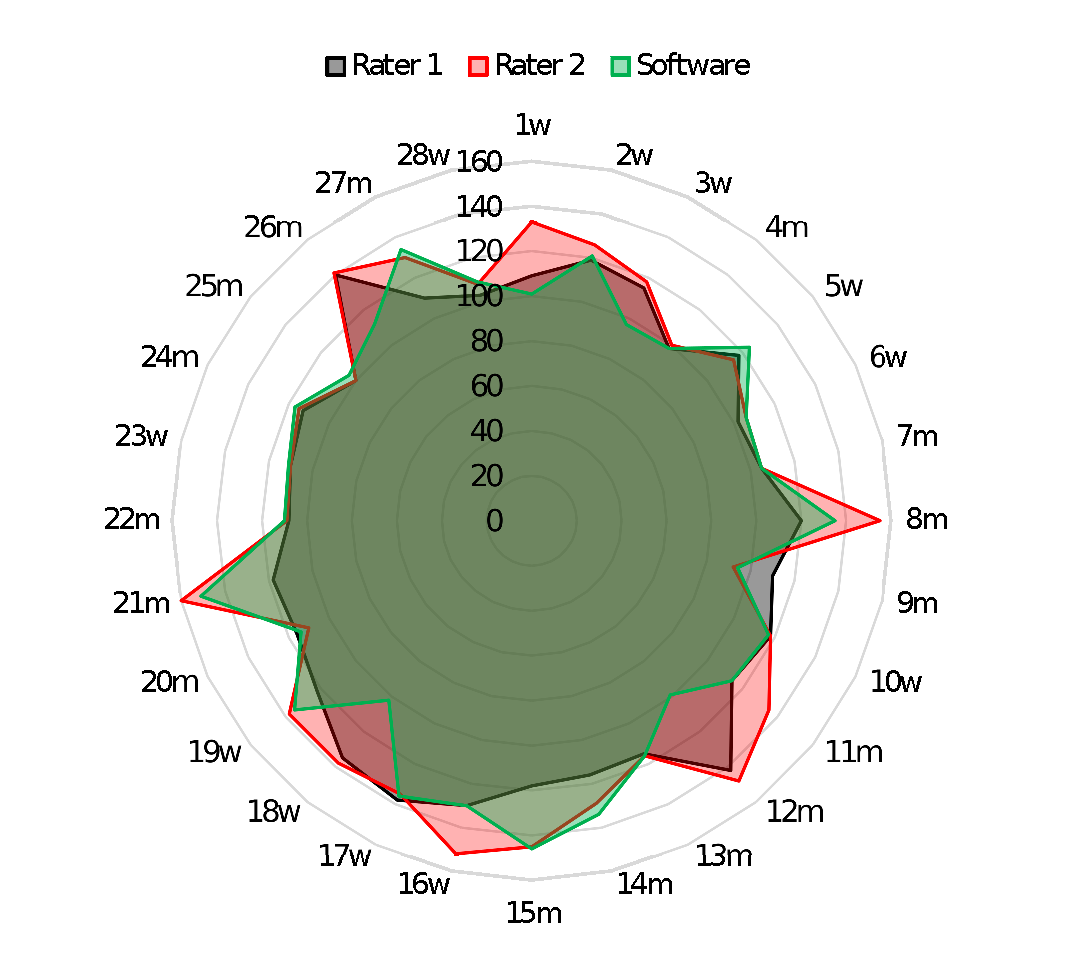
\includegraphics[scale=0.4]{Bilder/v-slope_net.eps}
			\subcaption[Vergleich der VT1-Bestimmungen durch V-Slope]{Vergleich der VT1-Bestimmungen durch V-Slope zwischen Ratern und Software; Intervall: \SIrange{0}{160}{\per\minute}}
			\label{subpic:pic1}
	\end{subfigure}%
	\hfil
	\begin{subfigure}[c]{0.45\textwidth}
		\centering
		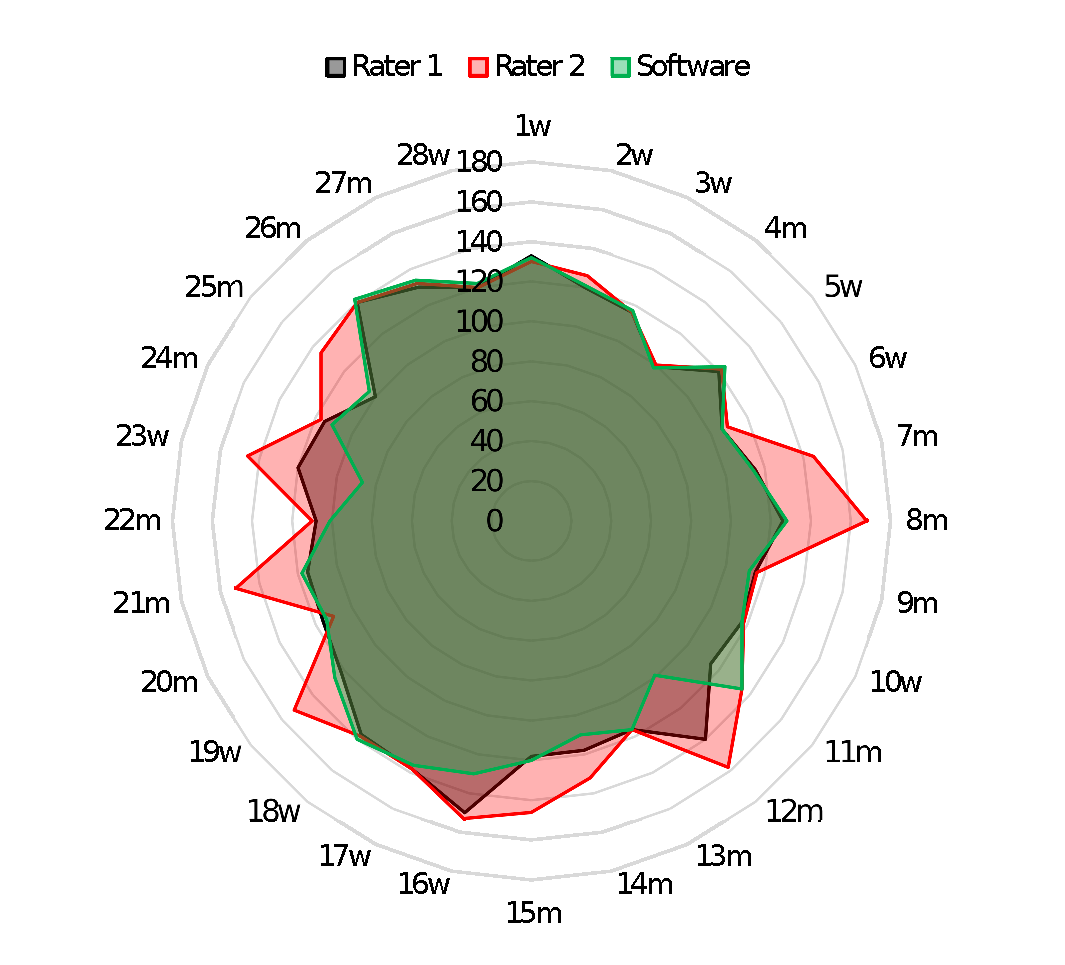
\includegraphics[scale=0.4]{Bilder/eqo2_net.eps}
			\subcaption[Vergleich der VT1-Bestimmungen durch das \gls{EQO2}]{Vergleich der VT1-Bestimmungen durch das \gls{EQO2} zwischen Ratern und Software; Intervall: \SIrange{0}{180}{\per\minute}}
			\label{subpic:pic2}
	\end{subfigure}
\caption[Grafische Darstellung der Übereinstimmung für die VT1]{Darstellung der Übereinstimmung zwischen Ratern und Software bei Bestimmung der VT1; Grau: Rater 1; Rot: Rater 2; Grün: Software; Kontrastierungen stellen Übereinstimmungen dar}
\label{pic:pic22}
\end{figure}
%
\begin{figure}[H]
	\centering
	%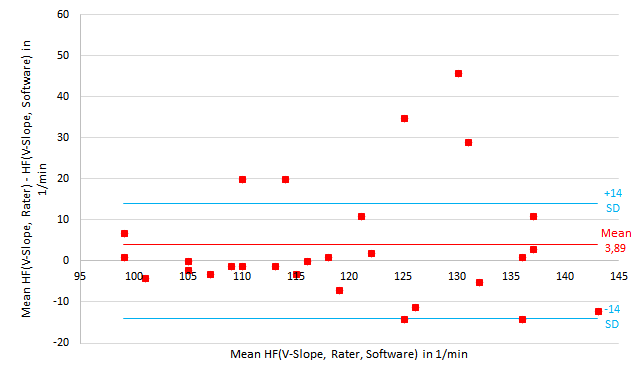
\includegraphics[scale=0.7]{Bilder/mean_vslope}
	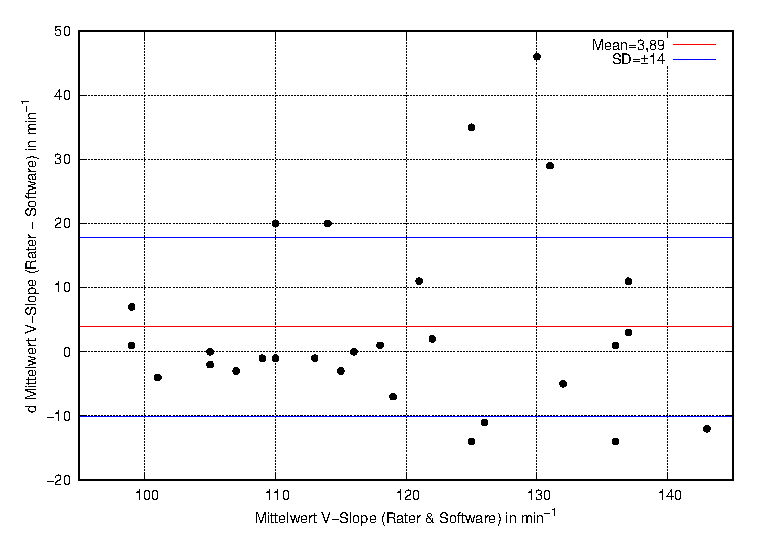
\includegraphics[scale=0.95]{Bilder/vslope.eps}
	\caption[Differenzen der V-Slope-Ergebnisse zwischen Ratern und Software]{Differenzen zwischen den Mittelwerten für die VT1 von Ratern und Software durch V-Slope; Mean = Mittelwert von $\Delta$ Rater-Software, SD~=~Standardabweichung}
	\label{pic:pic23}
\end{figure}
%
\begin{figure}[H]
	\centering
	%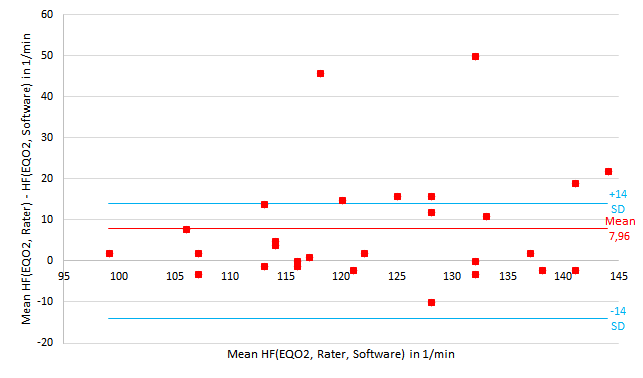
\includegraphics[scale=0.7]{Bilder/mean_eqo2}
	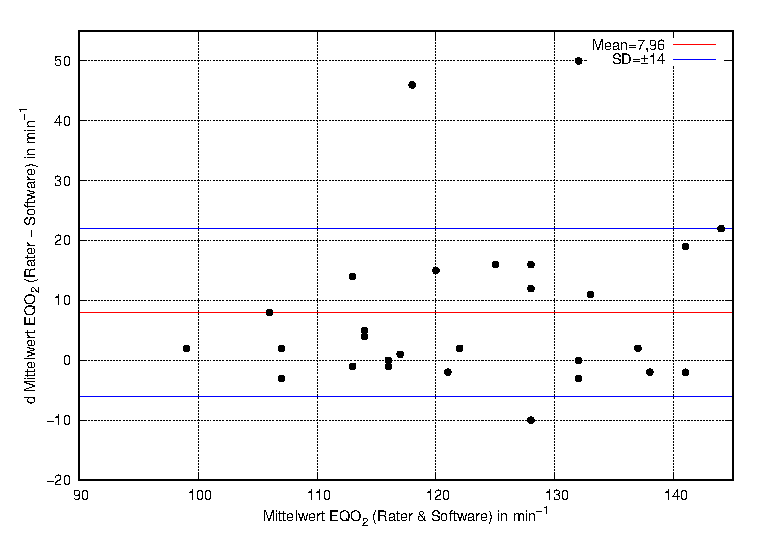
\includegraphics[scale=0.95]{Bilder/eqo2.eps}
	\caption[Differenzen der \gls{EQO2}-Ergebnisse zwischen Ratern und Software]{Differenzen zwischen den Mittelwerten für die VT1 von Ratern und Software durch das \gls{EQO2}; Mean = Mittelwert von $\Delta$ Rater-Software, SD~=~Standardabweichung}
	\label{pic:pic24}
\end{figure}
%
Um zu analysieren, wie stark die Ergebnisse der Rater von denen der Software im Mittel differieren, wurden für beide Methoden Punktdiagramme erstellt, in denen die Differenzen aus den gemittelten VT1-Werten der Rater und der Software gegen die Gesamtmittelwerte für alle 28 Personen aufgetragen wurden. In Abb. \ref{pic:pic23} ist das Diagramm für die V-Slope-Methode abgebildet. Der Mittelwert der Differenzen zwischen Ratern und Software ist als rote Linie ins Diagramm einfügt. Die Werte für die VT1, die von Ratern und Software mittels V-Slope bestimmt wurden, unterscheiden sich durchschnittlich um $3,89$ $\pm$14 Schläge pro Minute.\\
Abb. \ref{pic:pic24} zeigt das Diagramm für die \gls{EQO2}-Methode mit den Differenzen zwischen Ratern und Software. Dort beträgt diese im Mittel \SI{7,98}{\per\minute} $\pm$14 \si{\per\minute}.
%
\subsection{Ergebnisse für VT2}
%
\begin{table}[H]
	\begin{center}
		\caption{Ergebnisse für die \gls{HF} in \si{\per\minute} bei VT2}
		\medskip
		\begin{tabulary}{\textwidth}{L@{\hspace{3em}} C C C C C C C}
			\toprule
			& \multicolumn{2}{c}{\textbf{Rater 1}} & \multicolumn{2}{c}{\textbf{Rater 2}} & \multicolumn{3}{c}{\textbf{Software}} \\
			\midrule
			ID & \gls{EQCO2} & \gls{VE}/\gls{VCO2} & \gls{EQCO2} & \gls{VE}/\gls{VCO2} & \gls{EQCO2} & \gls{VE}/\gls{VCO2} & RQ=1 \\
			\midrule
			\midrule
			1w & 163 & 162 & 160 & 163 & 162 & 162 & 166 \\
			2w & 161 & 159 & 161 & 173 & 161 & 177 & 155 \\
			3w & 143 & 145 & 142 & 145 & 155 & 143 & - \\
			4m & 143 & 145 & 140 & 140 & 144 & 144 & - \\
			5w & 158 & 158 & 160 & 171 & 172 & 182 & 177 \\
			6w & 130 & 130 & 158 & 159 & 159 & 159 & 154 \\
			7m & 150 & 150 & 150 & 162 & 151 & 161 & 166 \\
			8m & 163 & 163 & 180 & 170 & 169 & 180 & 192 \\
			9m & 160 & 160 & 160 & 161 & 160 & 128 & 173 \\
			10w & 161 & 161 & 162 & 162 & 164 & 164 & 152 \\
			11m & 149 & 160 & 160 & 164 & 162 & 162 & 172 \\
			12m & 165 & 168 & 168 & 169 & 159 & 159 & - \\
			13m & 150 & 149 & 151 & 150 & 160 & 150 & - \\
			14m & 158 & 162 & 166 & 164 & 165 & 165 & 171 \\
			15m & 186 & 185 & 187 & 187 & 188 & 187 & - \\
			16w & 170 & 170 & 169 & 169 & 171 & 185 & 181 \\
			17w & 160 & 159 & 159 & 178 & 172 & 187 & 155 \\
			18w & 170 & 172 & 168 & 169 & 170 & 170 & 180 \\
			19w & 158 & 159 & 156 & 158 & 157 & 168 & 156 \\
			20m & 162 & 163 & 169 & 169 & 168 & 168 & 189 \\
			21m & 150 & 155 & 152 & 182 & 163 & 183 & - \\
			22m & 130 & 140 & 151 & 152 & 141 & 141 & - \\
			23w & 145 & 143 & 149 & 145 & 158 & 146 & - \\
			24m & 160 & 159 & 160 & 159 & 160 & 170 & 113 \\
			25m & 137 & 137 & 152 & 153 & 144 & 153 & - \\
			26m & 158 & 158 & 157 & 158 & 157 & 157 & 168 \\
			27m & 158 & 158 & 175 & 178 & 159 & 188 & 191 \\
			28w & 212 & 213 & 208 & 210 & 213 & 213 & 209 \\
			\bottomrule
		\end{tabulary}
		\label{tab:tabelle6}
	\end{center}
\end{table}
%
In Tab. \ref{tab:tabelle6} sind die Werte für die \gls{HF} eingetragen, an denen Rater und Software die VT2 bestimmt haben. In dieser Tabelle wurde die Software-Spalte zusätzlich mit der Referenzmethode RQ~=~1 ergänzt. Bei 9 von 28 Testmessungen konnte mit dieser Methode keine VT2 bestimmt werden, da die betroffenen Probanden dauerhaft einen RQ~<~1 besaßen.
%
\begin{figure}[H]
	\centering
	\begin{subfigure}[c]{0.45\textwidth}
		\centering
		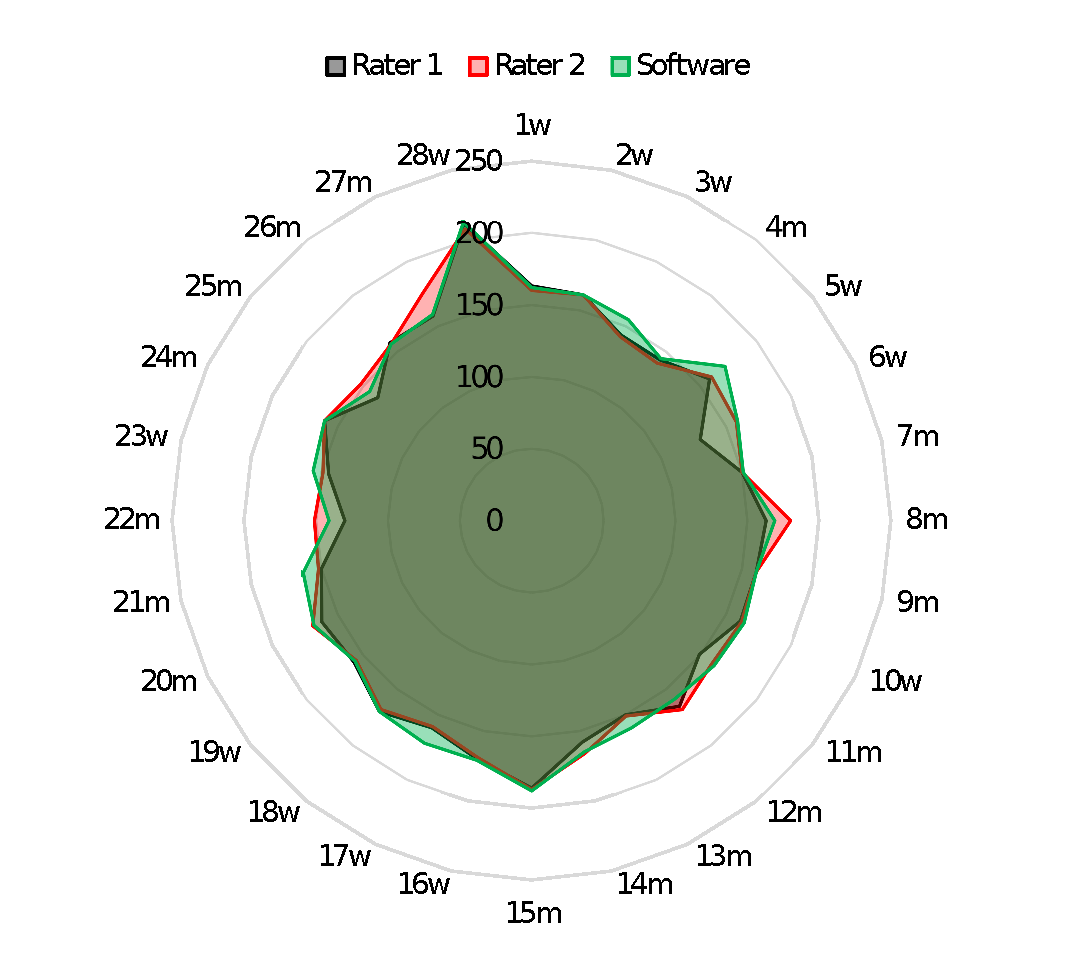
\includegraphics[scale=0.4]{Bilder/eqco2_net.eps}
		\subcaption[Vergleich der VT2-Bestimmungen durch das \gls{EQCO2}]{Vergleich der VT2-Bestimmungen durch das \gls{EQCO2} zwischen Ratern und Software; Intervall: \SIrange{0}{250}{\per\minute}}
		\label{subpic:pic3}
	\end{subfigure}%
	\hfil
	\begin{subfigure}[c]{0.45\textwidth}
		\centering
		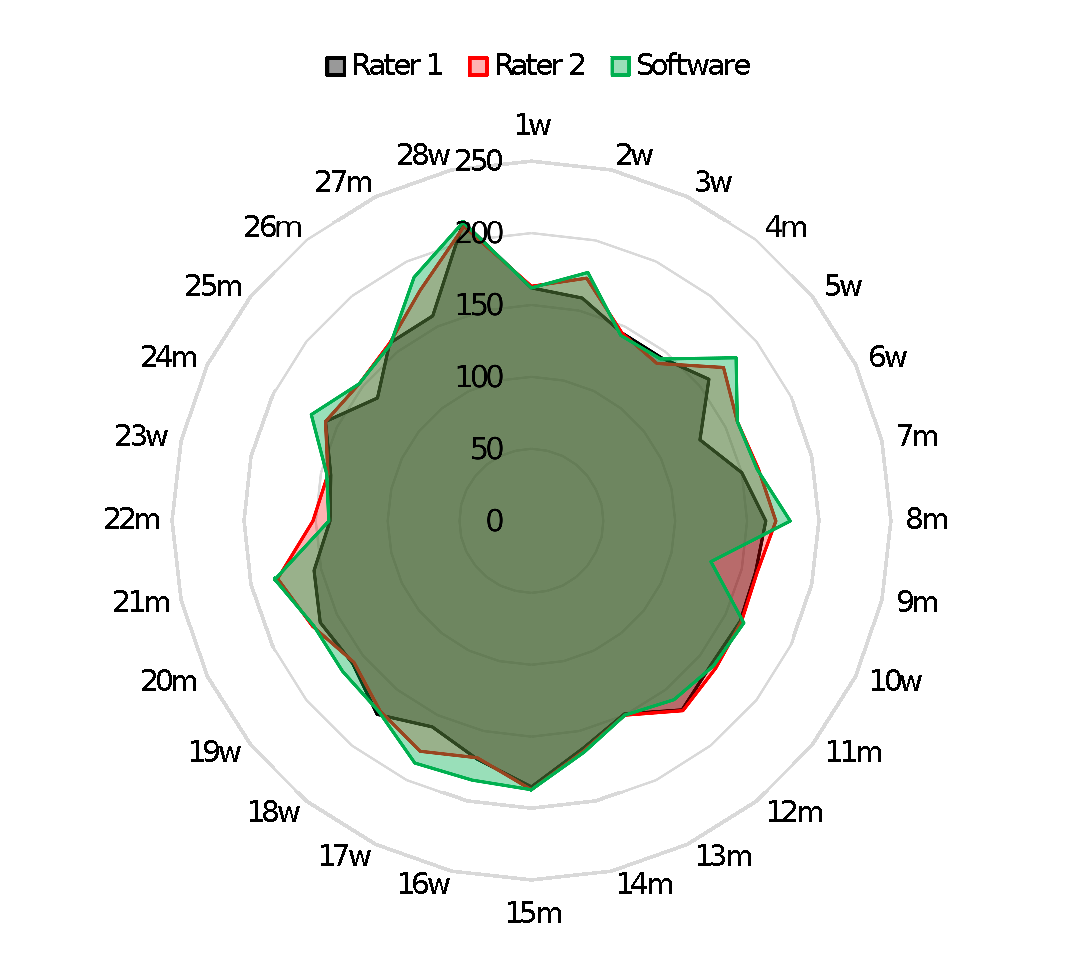
\includegraphics[scale=0.4]{Bilder/vevco2_net.eps}
		\subcaption[Vergleich der VT2-Bestimmungen durch \gls{VE}/\gls{VCO2}]{Vergleich der VT2-Bestimmungen durch \gls{VE}/\gls{VCO2} zwischen Ratern und Software; Intervall: \SIrange{0}{250}{\per\minute}}
		\label{subpic:pic4}
	\end{subfigure}
	\caption[Grafische Darstellung der Übereinstimmung für die VT2]{Darstellung der Übereinstimmung zwischen Ratern und Software bei Bestimmung der VT2; Grau: Rater 1; Rot: Rater 2; Grün: Software; Kontrastierungen stellen Übereinstimmungen dar}
	\label{pic:pic25}
\end{figure}
%
Abb. \ref{pic:pic25} zeigt die Netzdiagramme für die VT2-Ergebnisse durch das \gls{EQCO2} und \gls{VE}/\gls{VCO2}.

\begin{figure}[H]
	\centering
	%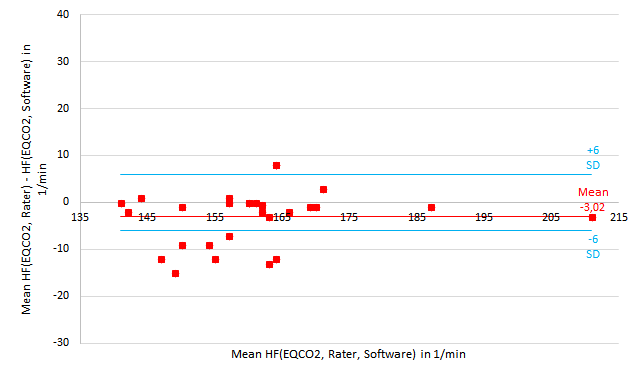
\includegraphics[scale=0.7]{Bilder/mean_eqco2}
	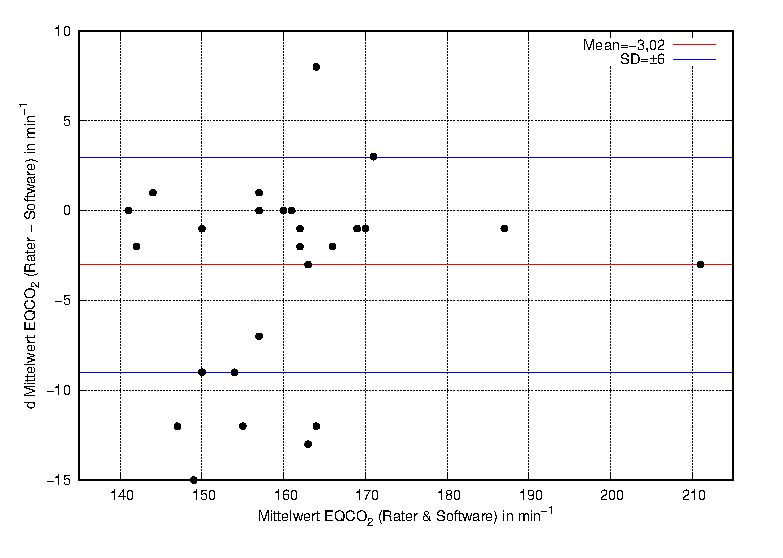
\includegraphics[scale=0.95]{Bilder/eqco2.eps}
	\caption[Differenzen der \gls{EQCO2}-Ergebnisse zwischen Ratern und Software]{Differenzen zwischen den Mittelwerten für die VT1 von Ratern und Software durch das \gls{EQCO2}; Mean = Mittelwert von $\Delta$ Rater-Software, SD~=~Standardabweichung}
	\label{pic:pic26}
\end{figure}
%
In Abb. \ref{pic:pic26} ist die Streuung der \gls{EQCO2}-Methode dargestellt. Die durchschnittliche Differenz für die VT2, basierend auf dem \gls{EQCO2}, beträgt \SI{-3,02}{\per\minute} $\pm$6 \si{\per\minute}.
%
\begin{figure}[H]
	\centering
	%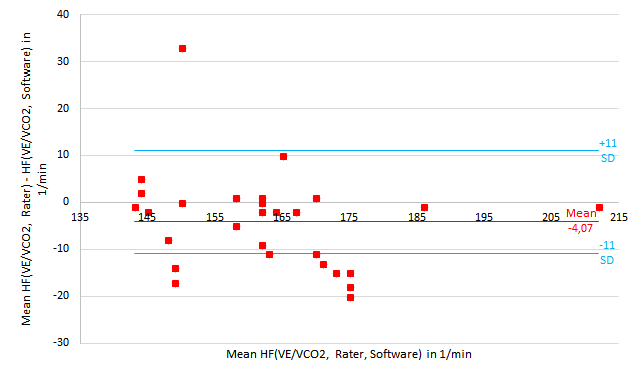
\includegraphics[scale=0.7]{Bilder/mean_vevco2}
	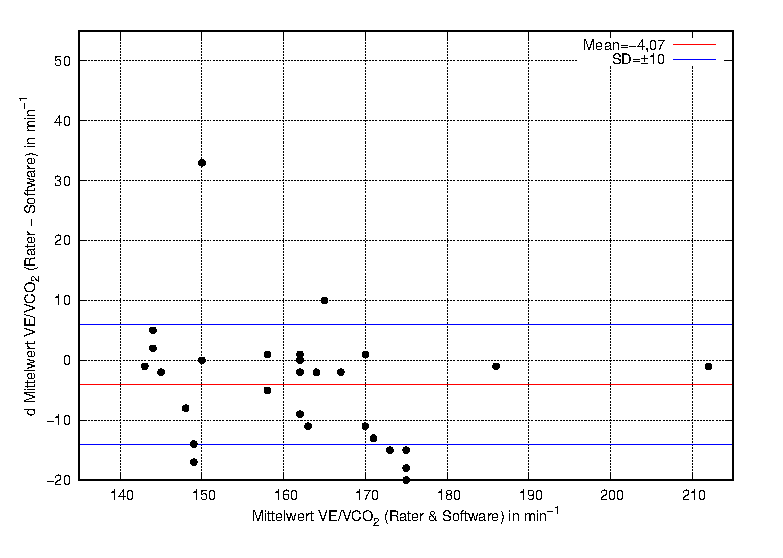
\includegraphics[scale=0.95]{Bilder/vevco2.eps}
	\caption[Differenzen der \gls{VE}/\gls{VCO2}-Ergebnisse zwischen Ratern und Software]{Differenzen zwischen den Mittelwerten für die VT1 von Ratern und Software durch \gls{VE}/\gls{VCO2}; Mean = Mittelwert von $\Delta$ Rater-Software, SD~=~Standardabweichung}
	\label{pic:pic27}
\end{figure}
%
Abb. \ref{pic:pic27} zeigt die Abweichungen der Ergebnisse für \gls{VE}/\gls{VCO2}. Hier differieren Rater und Software um durchschnittlich \SI{-4,07}{\per\minute} bei einer \gls{SD} von $\pm$10 \si{\per\minute}.
	\chapter{Diskussion}

In diesem Kapitel wird analytisch auf die vorangegangenen Resultate eingegangen und die Schwellenbestimmung der Rater und Software evaluiert. Im Zuge dessen werden die in Kapitel 1.3 aufgeführten Fragen chronologisch beantwortet:
%
\begin{tabbing}
	Ist die Spiroergometrie mit dem metabolicscan durchzuführen?\\
	Welche Methode zur Schwellenbestimmung ist optimal?\\
	Kann die VT2 mit den neuen Methoden genauer bestimmt werden, als mit RQ~=~1?
\end{tabbing}
%
Anschließend werden potentielle Fehlerquellen sowie eventuelle Defizite der Durchführung und Limitationen behandelt und diesbezüglich einige Vorschläge für die Firma cardioscan präsentiert.
%

\section{Spiroergometrie mit dem metabolicscan}

Da nach den Spiroergometrie-Tests für alle Probanden Plots generiert wurden, in denen die Veränderungen der \gls{VE}, \gls{VO2} und \gls{VCO2} erkennbar und nachvollziehbar waren, kann geschlussfolgert werden, dass der metabolicscan in Verbindung mit der \gls{CCPS} und Fahrradergometern grundsätzlich zur Durchführung der Spiroergometrie genutzt werden kann. Während der Messungen wurden keine Störungen oder Fehler der verbauten Sensoren festgestellt. Die maximal gemessene \gls{AF} bei den Testmessungen betrug \SI{52,5}{\per\minute} und liegt damit innerhalb der Grenzen des \gls{O2}-Sensors. Mit \SI{136,27}{\litre\per\minute} befindet sich auch die maximal gemessene \gls{VE} unterhalb des Maximums des Flowsensors. Der metabolicscan wurde vor dem Projekt mithilfe eines Lungensimulators bei Atemfrequenzen zwischen \SIlist{6;50}{\per\minute} und unterschiedlichen Gaskonzentrationen kalibriert, weswegen ausgeschlossen werden kann, dass die Sensoren fehlerhaft waren. Zudem wird jeder produzierte metabolicscan mithilfe einer Ausgleichskurve für die Flowmessung angepasst, die in die Gerätekalibrierung zu Beginn einer Messung implementiert ist. Dennoch können Abweichungen in der Messtechnik nicht vollkommen ausgeschlossen werden.\\
\clearpage
Alle Grafiken wurden bezüglich ihrer Qualität zunächst subjektiv und unbeeinflusst von anderen Personen in die Kategorien Gut und Kritisch einsortiert, um zu überprüfen, ob mit den Rohdaten des metabolicscan hinreichende Plots zur Schwellenbestimmung erstellt werden. Plots, die optisch mithilfe einer jeweiligen Methode direkt auszuwerten waren und außerdem keine schwerwiegenden Artefakte aufwiesen, wurden als gut deklariert. In die Rubrik Kritisch kamen jene Graphen, die beispielsweise unregelmäßige Kurvenverläufe aufwiesen und dadurch nur sehr differenziert evaluiert werden konnten. Tab. \ref{tab:tabelle7} zeigt die Kategorien und Zuordnungen.
%
\begin{table}[H]
	\begin{center}
		\caption{Kategorisierung der Plots nach Qualität}
		\medskip
		\begin{tabulary}{\textwidth}{L L C C}
			\toprule
			& & Gut & Kritisch \\
			\midrule
			\midrule
			\multirow{3}{1.5cm}{\textbf{VT1}} & V-Slope & 7 & 21 \\
			& \gls{EQO2} & 13 & 15 \\
			\cmidrule{2-4}
			& \textsl{Summe} & 20 (36 \%) & 36 (64 \%) \\
			\midrule
			\multirow{3}{1.5cm}{\textbf{VT2}} & \gls{EQCO2} & 21 & 7 \\
			& \gls{VE}/\gls{VCO2} & 15 & 13 \\
			\cmidrule{2-4}
			& \textsl{Summe} & 36 (64 \%) & 20 (36 \%) \\
			\bottomrule
		\end{tabulary}
		\label{tab:tabelle7}
	\end{center}
\end{table}
%
Mit 64~\% wurde der Großteil aller Plots zur Bestimmung der VT1 als kritisch bewertet. 21 von 28 und damit 75~\% der V-Slope-Graphen war optisch schwierig auszuwerten. Mit 15 von 28 bzw. 54~\% wurde auch die absolute Mehrheit der \gls{EQO2}-Kurven so bewertet. Bei den Methoden zur VT2-Bestimmung fiel die Wertung andersherum aus und 75~\% der \gls{EQCO2}- und 54~\% der \gls{VE}/\gls{VCO2}-Plots wurden in die Kategorie Gut eingeordnet. Insgesamt waren 64~\% der VT2-Plots gut auszuwerten.
%
\subsection{Kriterien für die optische Bewertung der Plots}
%
Nachfolgend werden Eigenschaften aufgelistet, anhand derer ein einzelner Plot als gut deklariert wurde. Um gut auswerten zu können, mussten die V-Slope-Kurven und die dazugehörigen \gls{HF}-Kurven differenzierbar sein. Nur so konnte der überproportionale Anstieg der \gls{VCO2} erkannt werden. War diese Eigenschaft nicht erfüllt, wenn es beim V-Slope für einen X-Wert mehrere Y-Werte gab, so wurde der Graph als kritisch bezeichnet. Einige V-Slopes besaßen allerdings auch sehr dicht beieinander gelegene Messpunkte, sodass Steigungsänderungen optisch schwierig zu erkennen waren. Auch diese Plots wurden als kritisch kategorisiert.\\
Bei guten \gls{EQO2}-Kurven wurde für die VT1-Bestimmung erwartet, dass sie einen eindeutig zu detektierenden Tiefpunkt besaßen, auf den eine von dort an stetige Zunahme folgte. Wenn die Kurven jedoch Schwankungen innehatten oder aber mehrere, optisch auf relativ gleicher Höhe liegende Tiefpunkte aufwiesen, waren sie kritisch.\\
Ähnliches galt für die VT2-Bestimmung mittels \gls{EQCO2}. Gut waren die Graphen, die eine annähernd Badewannen-ähnliche Form besaßen, sodass im fortgeschrittenen Messverlauf ein deutlich sichtbarer Anstieg zu erkennen war. Es wurden bei den Tests jedoch auch Plots generiert, in denen diese Kurven ebenfalls Schwankungen aufwiesen, sodass mehrere, potentiell als VT2 assoziierbare \gls{EQCO2}-Steigungen existierten. Diese Grafiken galten als kritisch.\\
Für \gls{VE}/\gls{VCO2} wurden ähnliche Voraussetzungen gestellt, wie für den V-Slope. Auch diese Graphen mussten differenzierbar sein und durften keine zackigen Verläufe annehmen. Auch hier sorgten einige Messpunkte mit optisch geringem Abstand für eine erschwerte, kritische Schwellenbestimmung. 
%
\section{Evaluierung der Methoden zur Schwellenbestimmung}
%
Die Kategorisierung wurde aus zeitlichen Gründen mit der ersten Version der grafischen Auswertung der Rohdaten vorgenommen. In Folge der Analyse der erstellten Grafiken wurde ein Fehler im MATLAB-Skript bei der Berechnung der \gls{AF} anhand des gemessenen Flows festgestellt. Es sollten zukünftig neue Testmessungen bzw. eine erneute Auswertung der neu generierten Plots durchgeführt werden, da die Erkenntnisse dadurch abweichen können. Dies lies allerdings der zeitliche Rahmen der Arbeit nicht zu.
%
\subsection{\gls{EQCO2} als optimale Methode}
%
75~\% der mit der ersten Algorithmus-Version generierten \gls{EQCO2}-Grafiken wurden jedoch bereits als gut kategorisiert. Die Ergebnisse dieser Methode brachte im Vergleich zwischen den Ratern sowie diesen und der Software die geringste Durchschnittsabweichung der VT2 mit \SI{-3,02}{\per\minute} $\pm$\SI{6}{\per\minute} hervor (siehe. Abb. \ref{pic:pic26}). Als zusätzliches Vergleichsinstrument wurde aus den Ergebnissen von Ratern und Software der Korrelationskoeffizient $r$ für jede Methode bestimmt. Je dichter $r$ am Wert eins liegt, desto mehr korrelieren die Schwellenbestimmungen und desto eindeutiger ist die Methode zur Schwellenbestimmung anwendbar. Mit $0,912$ ist der Korrelationskoeffizient für das \gls{EQCO2} sehr nah am Wert eins und im Vergleich mit den anderen Methoden am besten.
%
\begin{figure}[H]
	\centering
	%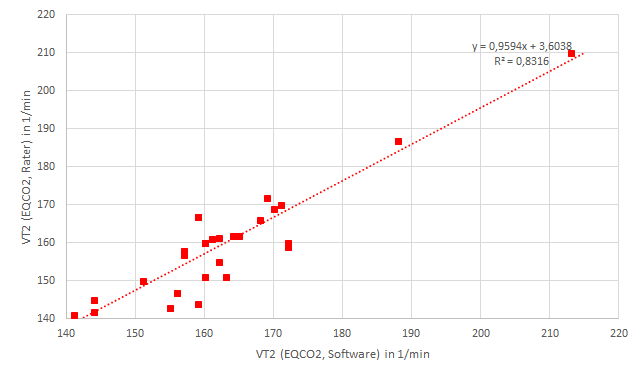
\includegraphics[scale=0.7]{Bilder/r_eqco2}
	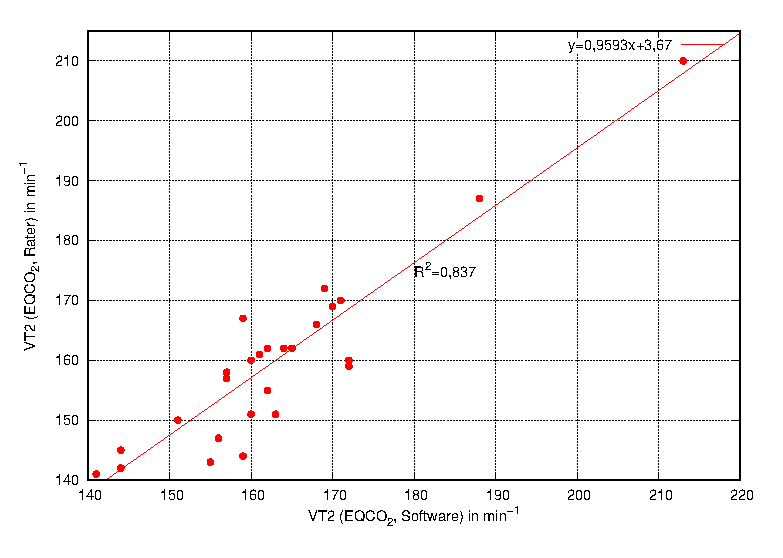
\includegraphics[scale=0.95]{Bilder/korr_eqco2.eps}
	\caption[Korrelation der \gls{EQCO2}-Werte von Ratern und Software]{Korrelation der mit dem \gls{EQCO2} bestimmten VT2 von Ratern und Software in Form einer Regressionsgeraden; aufgetragen wird die gemittelte VT2 der Rater gegenüber der VT2 der Software in \si{\per\minute}}
	\label{pic:pic28}
\end{figure}
%
Die Regressionsgerade in Abb. \ref{pic:pic28} zeigt die hohe Korrelation mit dem Bestimmheitsmaß $R^2 = 0,83$ zwischen Ratern und Software bei der mit \gls{EQCO2} bestimmten VT2 noch einmal grafisch.\\
Einen guten Plot stellt beispielhaft Abb. \ref{pic:pic20} dar, bei der ein deutlicher Anstieg der \gls{EQCO2}-Kurve beobachtet werden kann. In Abb. \ref{subpic:pic3} ist zu sehen, dass die Differenzen zwischen den beiden Ratern und auch zwischen den Ratern und der Software im Allgemeinen dennoch relativ gering waren. Die drei Netze liegen, im Ganzen betrachtet, relativ häufig sehr nah übereinander. Abb. \ref{pic:pic26} zeigt dazu, dass bei lediglich fünf Probanden Differenzen >\SI{10}{\per\minute} zu beobachten sind.\\
Interessant ist allerdings, dass in Abb. \ref{pic:pic17} bei Probandin 6w ein solch eindeutiger Anstieg des \gls{EQCO2} zu sehen ist, Abb. \ref{subpic:pic3} jedoch entnehmbar ist, dass zwischen Rater 1 und Rater 2 sowie der Software eine relativ große Differenz bei der Schwellenbestimmung existiert. Rater 1 detektierte die VT2 eine Stufe früher, wo in Abb. \ref{pic:pic17} bereits ein \gls{EQCO2}-Anstieg in der orangen Kurve zu sehen ist. Dieser war für Rater 2 eventuell noch nicht signifikant. Die Software bestimmte die VT2 später, da der Wert mit den Referenzdaten der HUNT 3 Studie mehr übereinstimmte. Die Mittelung der Werte je Stufe könnte hier zu einem leichten Anstieg zwischen zwei Messpunkten führen, der noch nicht auf das Exzess-\gls{CO2} zurückzuführen ist. Die Oxygen Delay Time $\tau$ zwischen Steigerung der Leistung zu Beginn einer neuen Stufe und der respiratorischen Reaktion beträgt bei kleinen Inkrementen ca. \SI{45}{\second}~\cite{Kroidl.2015}. Bei einer Stufendauer von \SI{2}{\minute} ist somit annehmbar, dass die physiologische Reaktion auf die Leistungssteigerung zu Beginn der Respirationsmessung nach \SI{90}{\second} bereits eingetreten ist und der Anstieg des \gls{EQCO2} könnte auf das Exzess-\gls{CO2} zurückzuführen sein. Vergleicht man die VT2 von Rater 1 bei \SI{130}{\per\minute} mit der \gls{HFmax} der Probandin bei \SI{178}{\per\minute}, entspricht die Schwelle 73~\%~\gls{HFmax}. Laut der HUNT 3 Studie liegt die durchschnittliche VT2 für gesunde Frauen zwischen 40 und 49 Jahren bei 90~\%~\gls{HFmax}$\pm$6~\%. Dementsprechend ist die VT2 von Rater 1 zu früh bestimmt worden.\\
Es gab wenige kritische \gls{EQCO2}-Kurven, in denen wechselnde Schwankungen zwischen positiver und negativer Steigung auftraten, sodass bei der optischen Auswertung die entscheidende \gls{EQCO2}-Zunahme nicht einfach erkennbar war. Dies ist beispielsweise bei Proband 8m in Abb. \ref{pic:pic18} der Fall. Die Kurve steigt im letzten Drittel des Plots zweimal an und fällt dazwischen einmal. Infolgedessen kam es zu unterschiedlichen Bestimmungen der VT2 durch die Rater, wie Abb. \ref{subpic:pic3} zeigt.
%
\subsection{\gls{VE}/\gls{VCO2} als geeignete Referenzmethode}
%
Die Abweichungen zwischen Ratern und Software beträgt für diese Methode im Mittel \SI{-4,07}{\per\minute} und die \gls{SD} $\pm$\SI{11}{\per\minute}. Verglichen mit der \gls{EQCO2}-Methode weisen die Ergebnisse größere Unterschiede auf und die Schwellenbestimmungen geschahen weniger eindeutig. Der Korrelationskoeffizient $r$ nimmt den Wert $0,816$ an. 15 von 28 Kurven für diese Methode waren gut. Ein Beispiel bietet Abb. \ref{pic:pic20} von Proband 20m. In der ersten Hälfte der Messung sind zwar einige sehr dicht gelegene Messpunkte zu erkennen, doch in der zweiten Hälfte, in der die VT2 angenommen werden kann, ist die Zunahme der \gls{VCO2} deutlich zu sehen. Rater und Software kamen bei dieser Grafik zu sehr ähnlichen Ergebnissen.\\
Einige Kurven waren jedoch kritisch, da nicht differenzierbar. Bei dieser Methode wirkten diese Artefakte sich allerdings nicht so stark auf die Schwellenbestimmung aus, da sie, wie z.B. in Abb. \ref{pic:pic21} zu erkennen, ausschließlich in der ersten Messhälfte auftraten. Im Bereich der VT2 waren die Verläufe der Graphen meistens gut auszuwerten.\\
Jedoch traten auch in Feld 4 häufiger Plots auf, bei denen die Messpunkte dicht beieinander lagen und nicht genau ersichtlich war, in welcher Stufe der erste Anstieg auftrat. Hier kann beispielhaft Abb. \ref{pic:pic19} von Proband 9m gesichtet werden. Da der Graph in Feld 4 recht linear verläuft, war die subjektive Auswertung erschwert und die Rater bestimmten die VT2 später als die Software, die erneut den Vorteil der mathematischen Detektion der Steigung innehat.\\
Für die Auswertung von \gls{VE}/\gls{VCO2} lässt sich schlussfolgern, dass sie in Verbindung mit Mittelwerten und Stufentests erschwert wird, da der Graph anfällig für Artefakte ist. Eine \gls{SD} von $\pm$11 \si{\per\minute} zeigt, dass häufig keine eindeutigen Ergebnisse erzielt werden und diese auch um die mittlere Abweichung sehr stark streuen. Die Software birgt auch bei dieser Methode allerdings den Vorteil, dass die mathematische Bestimmung von Steigungsänderungen gut gelingt und die Methode somit für Vergleiche nutzbar wird. Eine erneute Auswertung mit einem optimierten Algorithmus könnte zu verbesserten und mehr korrelierenden Ergebnissen führen. Gegebenenfalls kann diese Methode künftig als Referenzmethode für die VT2-Bestimmung in die Software integriert werden.
%
\subsection{Problematik bei der Bestimmung der VT1}
%
\subsubsection{V-Slope-Methode}
%
Wenn die V-Slopes und die zugeordneten \gls{HF}-Kurven nicht differenzierbar waren, wie beispielsweise ist den Plots in Abb. \ref{pic:pic18} und Abb. \ref{pic:pic21} erkennbar ist, war die subjektive Bestimmung der VT1 erschwert und die Grafik kritisch. Diese Problematik trat relativ häufig auf und wurde auch vom 2.~Rater moniert. Es lagen jedoch auch Grafiken vor, bei denen die Plots zwar differenzierbar waren, aber dennoch mehrere Schwankungen aufwiesen.\\
Ein Beispiel hierfür ist die Grafik von Proband 8m. In Abb. \ref{pic:pic18} ist ein nicht differenzierbarer V-Slope zu sehen, der mehrere Knickpunkte enthält. Eine Vielzahl an solchen Punkten begünstigt eine große Varianz an Werten für die VT1. Während Rater~1 den ersten Anstieg in der 2. Stufe bei \SI{120}{\per\minute} beobachtete, wurde er laut Rater~2 erst nach den Schwankungen der Werte in Stufe 6 bei \SI{155}{\per\minute} erkennbar. Die kritische Bewertung des Plots wird dadurch belegt. Abb. \ref{subpic:pic1} zeigt hierzu, dass Rater~1 und Rater~2 häufiger, wie bei Proband 8m, zu unterschiedlichen Ergebnissen kamen.\\
Auch differenzierbare und stetig steigende V-Slopes, die jedoch viele Messpunkte besaßen und dadurch stärker geglättet wurden, brachten ungleiche Ergebnisse durch Rater und Software hervor. Für Proband 9m bestimmte Rater~1 die VT1 früher als Rater~2 und die Software. Bei Betrachtung von Abb. \ref{pic:pic19} fällt auf, dass die Kurvenverläufe allgemein recht eben sind. Hier wird ein Vorteil der algorithmischen Auswertung deutlich, da die Software die größte Steigungsänderung mathematisch und daher eindeutig bestimmt. Allerdings erkennt sie Software keine eventuellen Ausreißer und kann den Trainingszustand einer Person nicht bewerten, der die Rater dazu veranlassen konnte, die VT1 im späteren Messverlauf zu vermuten.\\
21 von 28 V-Slope-Grafiken waren aufgrund dieser Gründe kritisch, was durch das Diagramm in Abb. \ref{subpic:pic1} und die darin sichtbaren Abweichungen zwischen den Schwellen belegt werden kann. Es ist durch recht viele hellrote Schraffuren im Diagramm zu erkennen, dass der 2.~Rater die VT1 meistens später bzw. bei höheren \gls{HF} bestimmte. Dadurch, dass die beiden Rater häufig zu ungleichen Ergebnissen kamen, gibt es bei den Mittelwerten oft große Streuungen, sodass die Differenz zwischen Ratern und Software größer wird (siehe Abb. \ref{pic:pic23}). Der Korrelationskoeffizient $r$ liegt bei $0,526$, was als mangelhaft zu werten ist. Die durchschnittliche Differenz zwischen Ratern und Software mit \SI{3,89}{\per\minute} (siehe. Abb. \ref{pic:pic23}) ist zwar recht niedrig, doch da bei einigen Plots sehr hohe Unterschiede zwischen den Ergebnissen auftraten, ist die \gls{SD} mit $\pm$\SI{14}{\per\minute} vergleichsweise hoch.
%
\subsubsection{\gls{EQO2}-Methode}
%
Abb. \ref{pic:pic17} zeigt beispielhaft eine Grafik, mit der die VT1 eindeutig bestimmbar war. Auf den Tiefpunkt nach der 2. Stufe folgt ein stetiger Kurvenanstieg, sodass dort der Bereich der VT1 assoziiert werden kann. Rater und Software kamen zu sehr ähnlichen Ergebnissen die maximal um \SI{4}{\per\minute} differierten (siehe. Tab. \ref{tab:tabelle5}).\\
Mit 15 Plots wies allerdings die Mehrheit aller generierten Grafiken Schwankungen im 2. Feld auf. Hierfür kann die Grafik von Proband 8m als Beispiel verwendet werden. Der Tiefpunkt der \gls{EQO2}-Kurve liegt in Abb. \ref{pic:pic18} erst zwischen Stufe 6 und 7. Hier bestimmte Rater 2 dementsprechend auch die VT1. Da allerdings an diesem Punkt auch die \gls{EQCO2}-Kurve ansteigt und ein sehr leichter Anstieg der \gls{EQO2}-Kurve bereits nach Stufe 2 auftritt, wo das \gls{EQCO2} noch nicht zunimmt, wurde die VT1 von Rater 1 und auch von der Software dort identifiziert.\\
Ein weiteres Beispiel einer solchen Differenz zwischen den Ratern liegt bei Proband 21m vor (siehe Abb. \ref{subpic:pic2}). Erneut kann diese durch die Schwankungen des \gls{EQO2} in der entsprechenden Abb. \ref{pic:pic21} begründet werden. Rater 1 und Software nahmen hier auch den ersten \gls{EQO2}-Anstieg als die VT1 an, während Rater 2 die Schwelle am tatsächlichen Wertetiefpunkt der Kurve bestimmte.\\
Obwohl die optische Bewertung der \gls{EQO2}-Kurven positiver ausfiel und mehr Plots als gut kategorisiert wurden, fällt $r$ mit $0,464$ schlechter aus, als beim V-Slope. Dies liegt daran, dass bei einigen Plots bzw. Probanden die Differenzen zwischen Ratern und Software sehr groß waren. Dementsprechend kann auch diese Methode nicht als gut bezeichnet werden. Die durchschnittliche Differenz der Ergebnisse beträgt \SI{7,96}{\per\minute} (siehe Abb. \ref{pic:pic24}) und ist im Vergleich mit den anderen Methoden am höchsten.
%
\subsubsection{Fazit zur VT1}
%
Letztlich zeigen die behandelten Beispielplots und die Diagramme in Abb. \ref{pic:pic23} und \ref{pic:pic24}, dass die Ergebnisse häufiger stark differieren und oftmals kein eindeutiger Bereich für die VT1 mittels V-Slope und \gls{EQO2} bestimmt werden kann, da viele Plots aufgrund von Schwankungen kritisch waren. Die Ergebnisse beider Methoden weisen jeweils eine \gls{SD} von $\pm$14 \si{\per\minute} auf. Die gemittelte Differenz zwischen Ratern und Software fällt bei der \gls{EQO2}-Methode größer aus, was an zwei sehr großen Differenzen mit \SIlist{46,50}{\per\minute} liegt, die den Gesamtdurchschnitt bei 28 Probanden stark beeinflussen. Die beiden Korrelationskoeffizienten liegen relativ mittig von null und eins und belegen somit, dass die algorithmischen sowie durch Rater bestimmten VT1 der Testmessungen aufgrund der häufig starken Differenzen nur bedingt in Zusammenhang zu bringen sind und die verwendeten Methoden dementsprechend mit dieser Art der Durchführung einer Leistungsdiagnostik nicht optimal sind.\\
Die Artefakte, welche sowohl in den V-Slope- als auch in den \gls{VE}/\gls{VCO2}-Plots auftraten, jedoch beim V-Slope wesentlich signifikanter waren, da sie im Bereich der annehmbaren VT1 entstanden, können inzwischen auf die fehlerhafte Berechnung der \gls{AF} durch den MATLAB-Algorithmus zurückgeführt werden. Eine Analyse der anhand der Rohdaten erstellten Matrizen in MATLAB im Falle von Proband 21 (siehe Abb. \ref{pic:pic21}) ergab, dass während der betroffenen Stufen 4 und 5 nur jeweils drei Atemzüge durch den Algorithmus erkannt wurden. Da sich die \gls{AF} auf die Berechnung der \gls{VCO2} und \gls{VO2} auswirkt, kam es dementsprechend zu verfälschten Werten. Der Algorithmus wurde in Bezug auf die Auswertung der Flow-Rohdaten angepasst und könnte inzwischen andere Plots generieren. Die Überprüfung dieser These steht allerdings aus und ist nicht Teil dieser Arbeit.
%
\subsection{Problematik von RQ = 1}
%
Tab. \ref{tab:tabelle6} belegt, dass die Methode RQ = 1 zur alleinigen Bestimmung der VT2 nicht sinnvoll ist. In Kapitel 1.3 wurde erwähnt, dass der RQ einst häufig zu früh den Wert eins überschritt und die Schwellenbestimmung dadurch fehlerhaft wurde. Dieser Fall trat bei den Ergebnissen der 28 Tests nicht auf. Dies ist jedoch dadurch begründet, dass bereits Ausgleichsgeraden durch die Entwicklungsabteilung in den Algorithmus implementiert wurden. Darüber hinaus wurde vor Start des Projektes ein Befehl aus der Ansteuerung der metabolicscan entfernt, der bewirkt hatte, dass dieser sich zwischen den einzelnen Belastungsstufen rekalibriert. Da jedoch bei einer Spiroergometrie durch den Probanden mehr \gls{CO2} exspiriert wird und die Räumlichkeiten währenddessen nicht belüftet werden, um Störungen des Flowsensors zu vermeiden, steigt entsprechend die \gls{CO2}-Konzentration der Luft. Dies konnte gemessen werden und wirkte sich somit auf die Kalibrierung des Geräts aus, sodass ungewollte Drifts in der RQ-Kurve entstanden.\\
Bei 9 von 28 Personen stieg der Wert stattdessen gar nicht über eins, sodass die VT2 gar nicht bestimmt werden konnte. Dennoch wurde bei diesen neun Probanden mit \gls{EQCO2} sowie \gls{VE}/\gls{VCO2} die VT2 detektiert. Bei zehn Personen, bei denen mit der Referenzmethode eine VT2 definiert werden konnte, weichen die Werte jedoch von den übrigen Methoden mit \SI{10}{\per\minute} oder mehr ab. Auch die Ausgleichskurven sorgten nicht dafür, dass die Mehrheit der Messergebnisse mit den übrigen Methoden vergleichbar wird. Der Algorithmus wird künftig aus der \gls{CCPS} entfernt und durch die genauere \gls{EQCO2}-Methode ersetzt.
%
\section{Plausibilitätsprüfung der Messwerte}
%
Für die Spiroergometrie existieren keine validen Methoden zur Plausibilitätskontrolle der Messwerte, weswegen sämtliche Rohdaten der Spiroergometrie nicht überprüft werden konnten. Empfohlen wird stattdessen zur groben Abschätzung der Vergleich von \gls{VE}-, \gls{VO2}- und Belastungszunahme, da zwischen diesen Parametern bis zum Erreichen der VT1 eine gewisse physiologische Proportionalität besteht. Für diese Abschätzung sollen zwei Faustformeln in der klinischen Spiroergometrie nutzbar sein, wobei $n$ die Anzahl der gefahrenen Stufen sei~\cite{Ruehle.2012}:
%
\begin{flalign}
\dot{V}E_{max}\hspace{1mm} \text{in \si{\litre\per\minute}} &= \SI{9}{\litre\per\minute} + n * \SI{9}{\litre\per\minute} \pm 10 \%
\label{eq:formel14}\\[1em]
\dot{V}O_{2max}\hspace{1mm} \text{in \si{\milli\litre\per\minute}} &= 5 * \left\lbrace m\right\rbrace \text{in \kilogram} * W_{max}\hspace{1mm} \text{in \watt} * \SI{10}{\milli\litre\per\minute} \pm 10 \%
\label{eq:formel15}
\end{flalign}
%
\gls{VE} und \gls{VO2} sollen demnach einen idealerweise linearen Verlauf über die Leistung annehmen. Da die Berechnungen jedoch kaum anthropometrischen Daten oder individuellen Trainingszustände einbeziehen, wurde auf die mathematische Art der Überprüfung wegen der großen Varianz an Trainingszuständen in dieser Arbeit verzichtet. Allerdings kann mithilfe eines grafischen Vergleichs der Parameter der Verlauf einer Messung analysiert und bewertet werden.\\
In den Feldern 5 und 6 der in Kapitel 3 abgebildeten 6-Felder-Grafiken wurden die \gls{VE} und die \gls{VO2} hierfür jeweils der \gls{W} gegenübergestellt. Einige dieser Felder weisen allerdings analoge Schwankungen zu denen in Feld 1 und 4 auf und können empirisch ebenfalls mit der fehlerhafte Atemzugerkennung erklärt werden. Als alternative Plausibilitätskontrolle wurde stattdessen der Vergleich mit den Daten der HUNT 3 Studie angestellt, wie in Tab. \ref{tab:tabelle8} aufgeführt.\\
In der Tabelle werden die gemessenen \gls{VO2max}-Werte der einzelnen Probanden mit den Referenzwerten der entsprechenden Alterklasse sowie des Geschlechts aus der HUNT 3 Studie verglichen~\cite{Loe.2014}. Von 28 Probanden lagen 13 ober- oder unterhalb des entsprechenden Durchschnitts. Es muss jedoch hier berücksichtigt werden, dass die HUNT 3 Studie auf Laufbändern durchgeführt wurde. Bei der Laufbandergometrie liegt die \gls{VO2max} generell höher, da die Muskelgruppen und deren Wirkungsgrad sich zur Fahrradergometrie unterscheiden~\cite{Kroidl.2015}. Unter diesem Aspekt besteht eine geringere Vergleichbarkeit, da die restlichen 15 Probanden sich jedoch innerhalb des Durchschnittsbereichs bzw. der \gls{SD} befanden, kann diese Kontrolle zumindest differenziert einen Aufschluss über den hinreichenden Abschluss einer Spiroergometrie geben. 
%
\begin{table}[H]
	\centering
	\caption{Vergleich der innerhalb der Testmessungen erhobenen \gls{VO2max} mit Daten der HUNT 3 Studie, abhängig von Geschlecht und Alter}
	\medskip
	\begin{tabulary}{\textwidth}{L C C C}
		\toprule
		ID & \gls{VO2max} in \si{\litre\per\minute} & Ref.-\gls{VO2max} in \si{\litre\per\minute} $\pm$\gls{SD} & Vergleich \\
		\midrule
		\midrule
		1w & 2,4 & 2,62 $\pm$0,44 & unterer Durchschnitt \\
		2w & 2,1 & 2,77 $\pm$0,47 & niedriger \\
		3w & 2,7 & 2,74 $\pm$0,5 & Durchschnitt \\
		4m & 3,6 & 4,0 $\pm$0,62 & unterer Durchschnitt \\
		5w & 2,15 & 2,77 $\pm$0,47 & niedriger \\
		6w & 2,55 & 2,62 $\pm$0,44 & unterer Durchschnitt \\
		7m & 3,3 & 4,2 $\pm$0,65 & niedriger \\
		8m & 4,0 & 4,3 $\pm$0,73 & unterer durchschnitt \\
		9m & 4,05 & 4,0 $\pm$0,62 & oberer Durchschnitt \\
		10w & 2,78 & 2,77 $\pm$0,47 & oberer Durchschnitt \\
		11m & 2,6 & 4,3 $\pm$0,73 & niedriger \\
		12m & 4,0 & 4,2 $\pm$0,65 & unterer Durchschnitt \\
		13m & 3,45 & 4,3 $\pm$0,73 & niedriger \\
		14m & 3,85 & 4,3 $\pm$0,73 & unterer Durchschnitt \\
		15m & 4,05 & 4,3 $\pm$0,73 & unterer Durchschnitt \\
		16w & 2,98 & 2,77 $\pm$0,47 & oberer Durchschnitt \\
		17w & 2,0 & 2,77 $\pm$0,47 & niedriger \\
		18w & 2,7 & 2,77 $\pm$0,47 & Durchschnitt \\
		19w & 2,13 & 2,62 $\pm$0,44 & niedriger \\
		20m & 2,83 & 4,3 $\pm$0,73 & niedriger \\
		21m & 3,4 & 4,3 $\pm$0,73 & niedriger \\
		22m & 3,05 & 4,0 $\pm$0,62 & niedriger \\
		23w & 3,18 & 2,62 $\pm$0,44 & höher \\
		24m & 2,83 & 4,0 $\pm$0,62 & niedriger \\
		25m & 3,15 & 3,61 $\pm$0,6 & unterer Durchschnitt \\
		26m & 3,5 & 4,2 $\pm$0,65 & niedriger \\
		27m & 3,58 & 4,2 $\pm$0,65 & unterer Durchschnitt \\
		28w & 2,5 & 2,74 $\pm$0,5 & unterer Durchschnitt \\
		\bottomrule
	\end{tabulary}
	\label{tab:tabelle8}
\end{table}
%
\section{Potentielle Fehlerquellen bei der Spiroergometrie}
%
\subsection{Probandenbedingte Faktoren}
%
Bei der Spiroergometrie können Probanden die Ergebnisse negativ beeinflussen, indem sie ihre Atmung durch die ungewohnten Bedingungen stark verändern, sodass diese unphysiologisch wird. Bei wenigen Personen konnte mithilfe von Feld 5 und 6 beobachtet werden, dass sie zu Beginn der Leistungsdiagnostik eine recht hohe \gls{VE} besaßen und die \gls{AF} schnell zunahm. Da eine erneute Kompilierung z.B. bei Proband 21m nicht für bessere Plots in Feld 5 und 6 sorgte, resultiert dies aus einem anderen Fehler. Dieser kann auf das Mundstück bzw. den Bakterienfilter zurückgeführt werden. Durch diesen erhöht sich der Atemwiderstand, dessen Höhe von jeder Person subjektiv anders wahrgenommen wird. 7 der 28 Probanden empfanden die Ergonomie des Mundstücks als unangenehm und deuteten nach dem Test an, dass dieses die Atmung gerade zu Beginn einer Messphase erschwert habe. Dadurch neigten die Probanden dazu, tiefer und gleichzeitig schneller zu atmen. Infolgedessen stieg die \gls{VE} relativ zur \gls{VO2} höher, da der Körper zu diesem Zeitpunkt noch nicht die große Menge an aufgenommenem \gls{O2} verwerten konnte. Des Weiteren können Fehler entstehen, wenn Personen das Mundstück nicht rechtzeitig zu Munde führen. Einer Probandin rutschte das Mundstück bei erhöhter Belastung sogar mehrmals aus dem Mund. Die Dauer der Messphase beträgt stets \SI{30}{\second}. Zu Beginn einer Leistungsdiagnostik bei geringer Leistung ist die \gls{AF} bei den meisten gesunden Menschen noch recht niedrig. Die durchschnittliche \gls{AF} eines Erwachsenen in Ruhe beträgt ca. \SIrange{7}{20}{\per\minute}~\cite{Larsen.2017}. Kommt es zu Problemen mit dem Mundstück, sodass gewisse Schwellwerte bei der Atemzugerkennung der Software nicht überschritten und weniger Atemzüge erfasst werden, wird die gemittelte \gls{AF} und dadurch auch die \gls{VE} kleiner. Das wiederum kann zu veränderten Plots führen, wenn auf einen kleineren Mittelwert in der nächsten Stufe ein normaler folgt, wodurch die Steigung zwischen diesen zwei Punkten verfälscht wird und nicht mehr den ventilatorischen Reaktionen des Körpers entspricht. Zuletzt muss die Ernährung unmittelbar vor einer Spiroergometrie berücksichtigt werden (siehe Kapitel 2.1.2). Zwar wird zukünftig der RQ nicht mehr für die Schwellenbestimmung verwendet, jedoch sollte der Grund-Laktat-Gehalt nicht durch erhöhte Zuckerzufuhr erhöht werden, um die Ausgangsbedingungen in Bezug auf die \gls{VCO2} zu normalisieren.
%
\subsection{Anwenderbedingte Faktoren}
%
Durch den Anwender der Spiroergometrie können ebenfalls Fehler verursacht werden. Beispielsweise kann oben genannter zeitlicher Verzug auch entstehen, wenn der Anwender dem Probanden das Mundstück zu spät reicht, sodass die Atemzugerfassung ebenfalls verfälscht wird. Schon eine falsche Vorbereitung der Belastungsphase kann zu Fehlern führen, wenn z.B. die Sattelhöhe nicht korrekt justiert oder ein unpassendes Belastungsprotokoll bestimmt wurde. Es ist wichtig, dass der Anwender im Vorwege den Trainingszustand einer Person korrekt einschätzen kann, um entsprechende Anpassungen am Protokoll vorzunehmen. Allerdings ist hier auch die deutliche Kommunikation mit dem Probanden zwingend erforderlich.
%
\subsection{Umweltbedingte Faktoren}
%
Wie in Kapitel 2.1.2 erwähnt, sind die Messbedingungen für eine Respirationsanalyse einzuhalten. Raumtemperatur und \gls{CO2}-Gehalt in der Luft wirken sich auf die \gls{HF} und \gls{La-}-Kinetik aus, was ebenfalls im Falle einer Nichtbeachtung zu Fehlern führt. Jedoch wurde der Raum vor jedem Test belüftet und die Temperatur im Toleranzbereich zwischen \SIrange{18}{22}{\degreeCelsius} gehalten. Die \gls{CO2}-Belastung der Atemluft in $10^{-6}$ (parts per million) wurde durch ein Messgerät sehr genau überprüft, um sicherzustellen, dass die Kalibrierung des metabolicscan vor jedem Test auf denselben Grundbedingungen basierte.
%
\section{Limitation}
%
Das Projekt war limitiert durch eine relativ kleine Teilnehmerzahl und dadurch sehr ungleiche Verteilung der unterschiedlichen Probandengruppen. Um die Aussagekraft der Ergebnisse zu erhöhen und diese beispielsweise besser mit der HUNT 3 Studie vergleichen zu können, wäre eine deutlich größere Probandengruppe notwendig gewesen. Die HUNT 3 Studie ist jedoch auch nicht optimal, da die Werte für Fahrrad- und Laufergometrie, wie bereits angedeutet, verschieden sind. Verlässliche Studien zur Fahrradergometrie mit großer Probandenzahl liegen jedoch momentan nicht vor.\\
Die Evaluierung war auch durch eine kleine Menge an wertenden Personen und einen gleichzeitigen Mangel an validen Referenzwerten eingeschränkt. Generell sind Normwerte im Bereich der Sportwissenschaft schwer zu definieren, da die Individualität an Zuständen zu groß ist. Dies bedeutet, dass bei der Analyse der individuellen Leistungsfähigkeit noch sensibler auf eventuelle Einflussfaktoren eingegangen werden muss, als beispielsweise bei einer rein medizinischen Lungenfunktionsmessung, der einige Normbereiche für z.B. die \gls{FEV1} oder \gls{FVC} zu Grunde liegen, welche anatomisch abgegrenzt sind.
%
\section{Ausblick und Handlungsempfehlung}
%
Ausgehend von den Ergebnissen dieser Arbeit wurde mit dem \gls{EQCO2} eine neue Methode für die VT2-Bestimmung erarbeitet, welche weiter optimiert zukünftig als Algorithmus die Basis für die Auswertung durch die \gls{CCPS} darbieten kann. In Verbindung mit dem Trainingszonenmodell nach Wilfried Kindermann können mit dieser Methode die Ziele der Firma cardioscan umgesetzt werden. Das Leistungsdiagnostik-Setup bietet jedoch Optimierungsmöglichkeiten. Zum Ersten wären eventuell Alternativen zu dem Mundstück, z.B. in Form einer Maske sinnvoll, da die Ergonomie des Mundstücks moniert wurde. Hier könnten weitere Tests mit alternativen Komponenten durchgeführt werden. Zum Zweiten gestaltet sich die Mittelung der Messwerte über die Gesamtanzahl an Atemzügen pro Stufe als nicht optimal, da dadurch die vorangegangen beschriebenen Verfälschung der Plots auftreten können. Eine gänzliche "`breath-by-breath"'-Auswertung jedes Atemzugs sollte wegen der zu großen Datenmenge zwar auch nicht in Betracht bezogen werden, jedoch könnten alternative Mittelungsverfahren (z.B. die "`gleitende"' Mittelung~\cite{Kroidl.2015}) getestet werden.\\
Die algorithmische Auswertung könnte für die anschließende Interpretation optimiert werden, indem z.B. ein Algorithmus programmiert wird, der ein Abflachen der \gls{HF}-Kurve zum Ende einer Leistungsdiagnostik überprüft. Dies könnte den Anwender dabei unterstützen, zu bewerten, ob eine Person tatsächlich ausbelastet ist. In der HUNT 3 Studie wurde ermittelt, bei wie viel Prozent der \gls{HFmax} die VT2 einer Person erreicht worden war. Eine abflachende \gls{HF}-Kurve wäre ein Indikator für das Erreichen der \gls{HFmax}. Durch einen Vergleich der \gls{HF} bei der VT2 und der \gls{HFmax} könnten Ergebnisse zusätzlich evaluiert werden.\\
Zum Abschluss bleibt zu erwähnen, dass trotz algorithmischer Auswertung einer Spiroergometrie eine Interpretation der Ergebnisse seitens einer Person mit Fachwissen unabdingbar ist. Die gezeigten Grafiken, anhand derer die Schwellen bestimmt wurden, bieten lediglich die Grundlage und müssen in ein optimiertes Interface der \gls{CCPS} implementiert werden. Die komplette Thematik der Atemgasanalyse ist im Allgemeinen sehr komplex und sollte daher nicht von ungeschultem Personal behandelt werden. cardioscan betreibt für alle diagnostischen Anwendungen eine Academy, welche in regelmäßigen Intervallen Seminare und Workshops durch Schulungsreferenten und -referentinnen beim Kunden durchführen lässt. Bei diesen Seminaren sollten auch die Details der Vorbereitung behandelt werden. Die Software könnte die Anwender auch auf diesem Wege unterstützen, indem z.B. der Timer im Interface durch einen Hinweis ergänzt wird, der daran erinnert, das Mundstück zur Messung vorzubereiten, um Messfehler zu reduzieren.
%
\nocite{*}

%\printnomenclature

%\bibliography{Referenzen}
\printbibliography


		
	\appendix
	\chapter{Technische Daten des Flowsensors}
\includepdf[pages=3]{Anhang/FS6122H.pdf}

\chapter{Technische Daten des \acrshort{CO2}/\acrshort{O2}-Sensor-Moduls}
\includepdf[pages=3-7]{Anhang/AION.pdf}

\chapter{Programmcode des MATLAB-Programms}
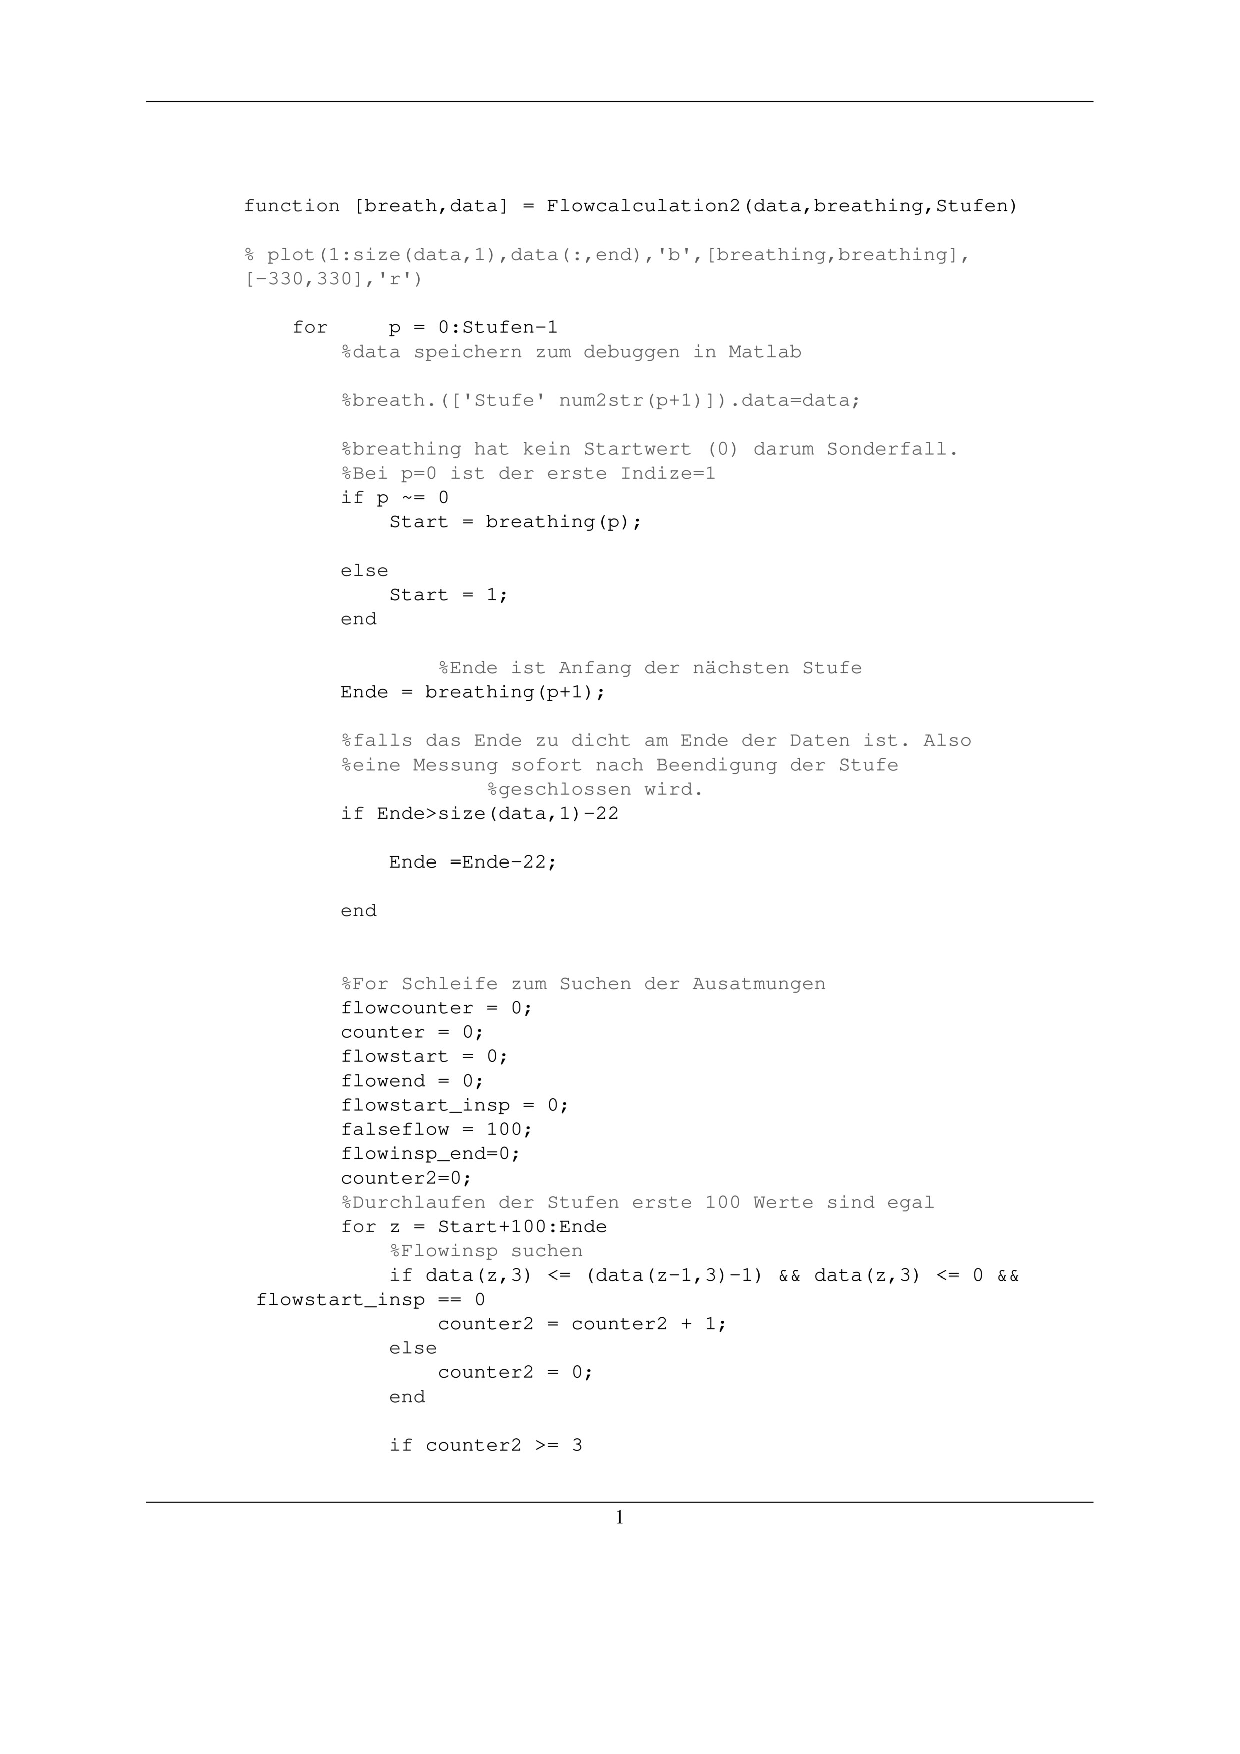
\includepdf[pages=-]{Anhang/Flowcalculation2.pdf}
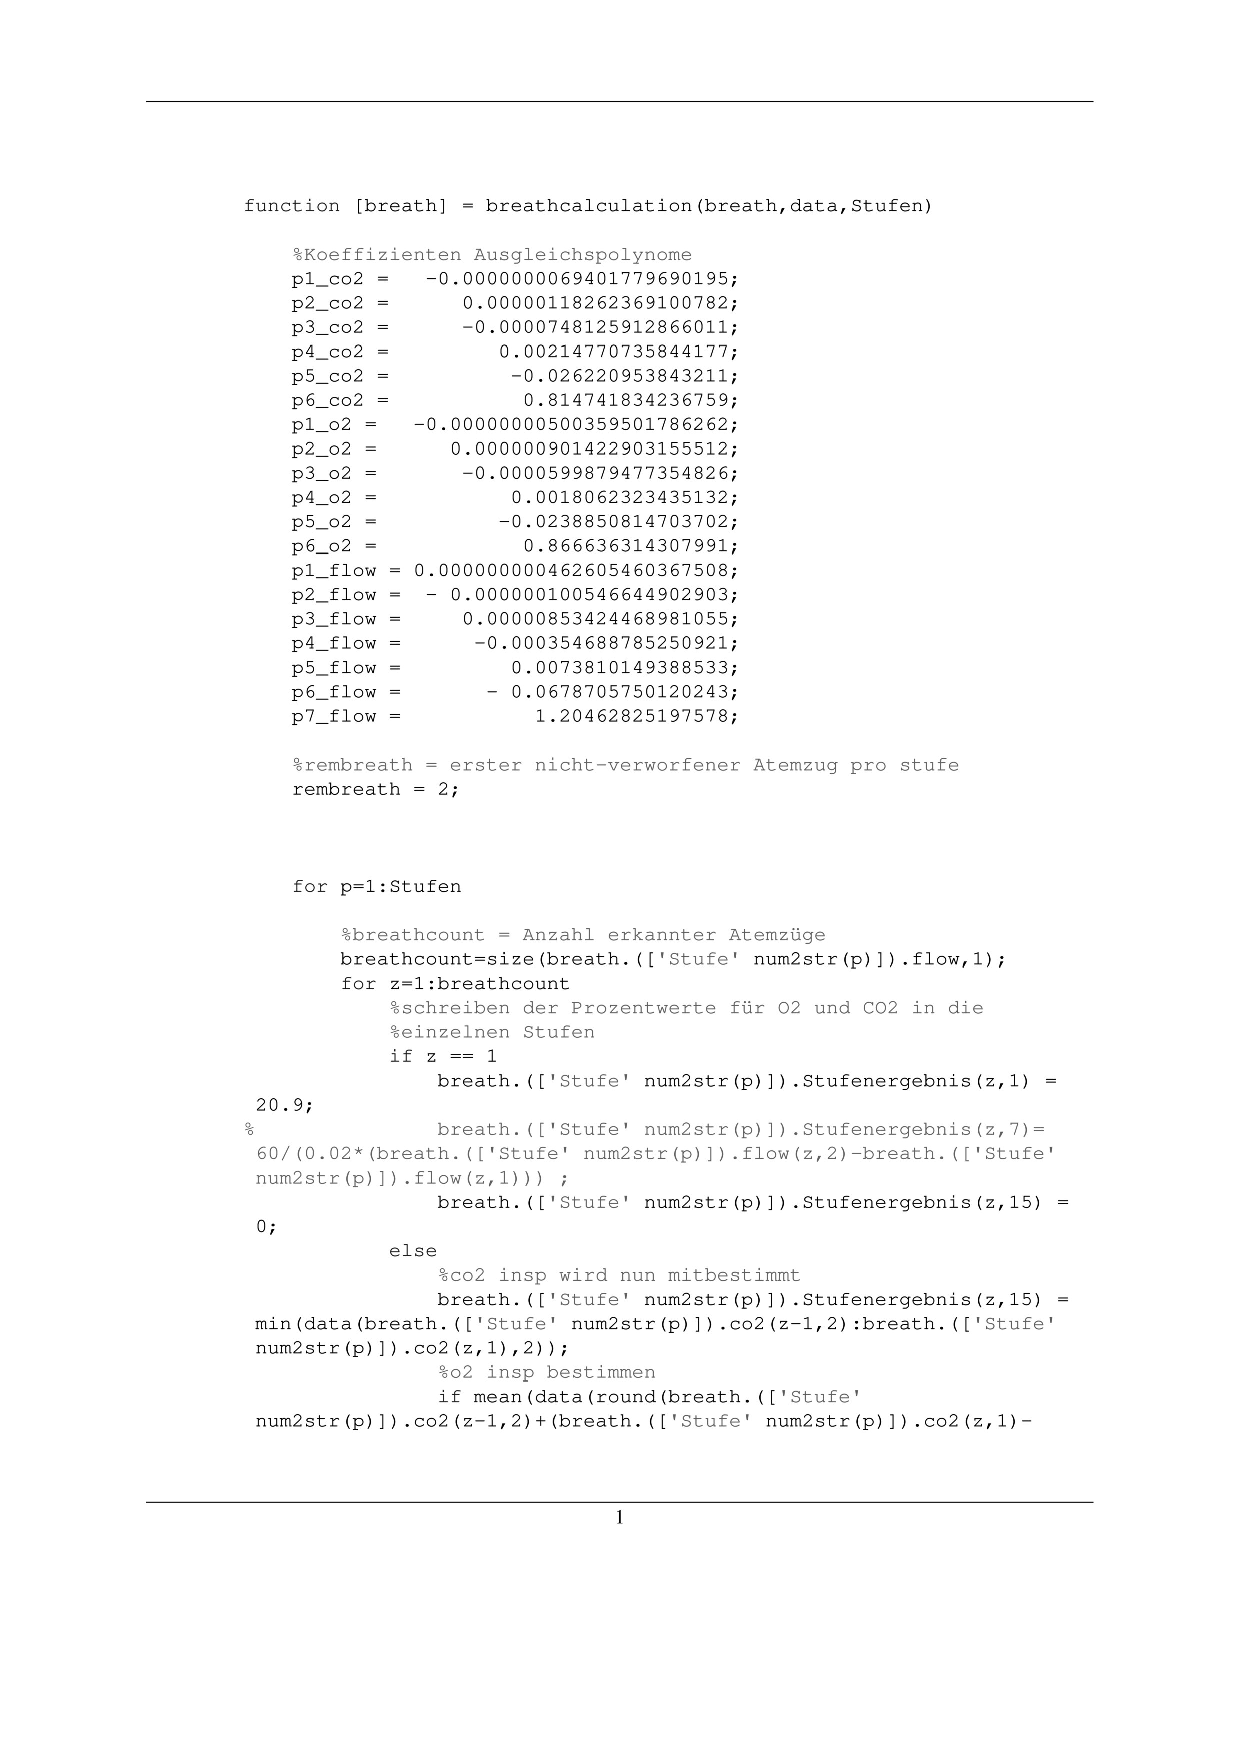
\includepdf[pages=-]{Anhang/breathcalculation.pdf}
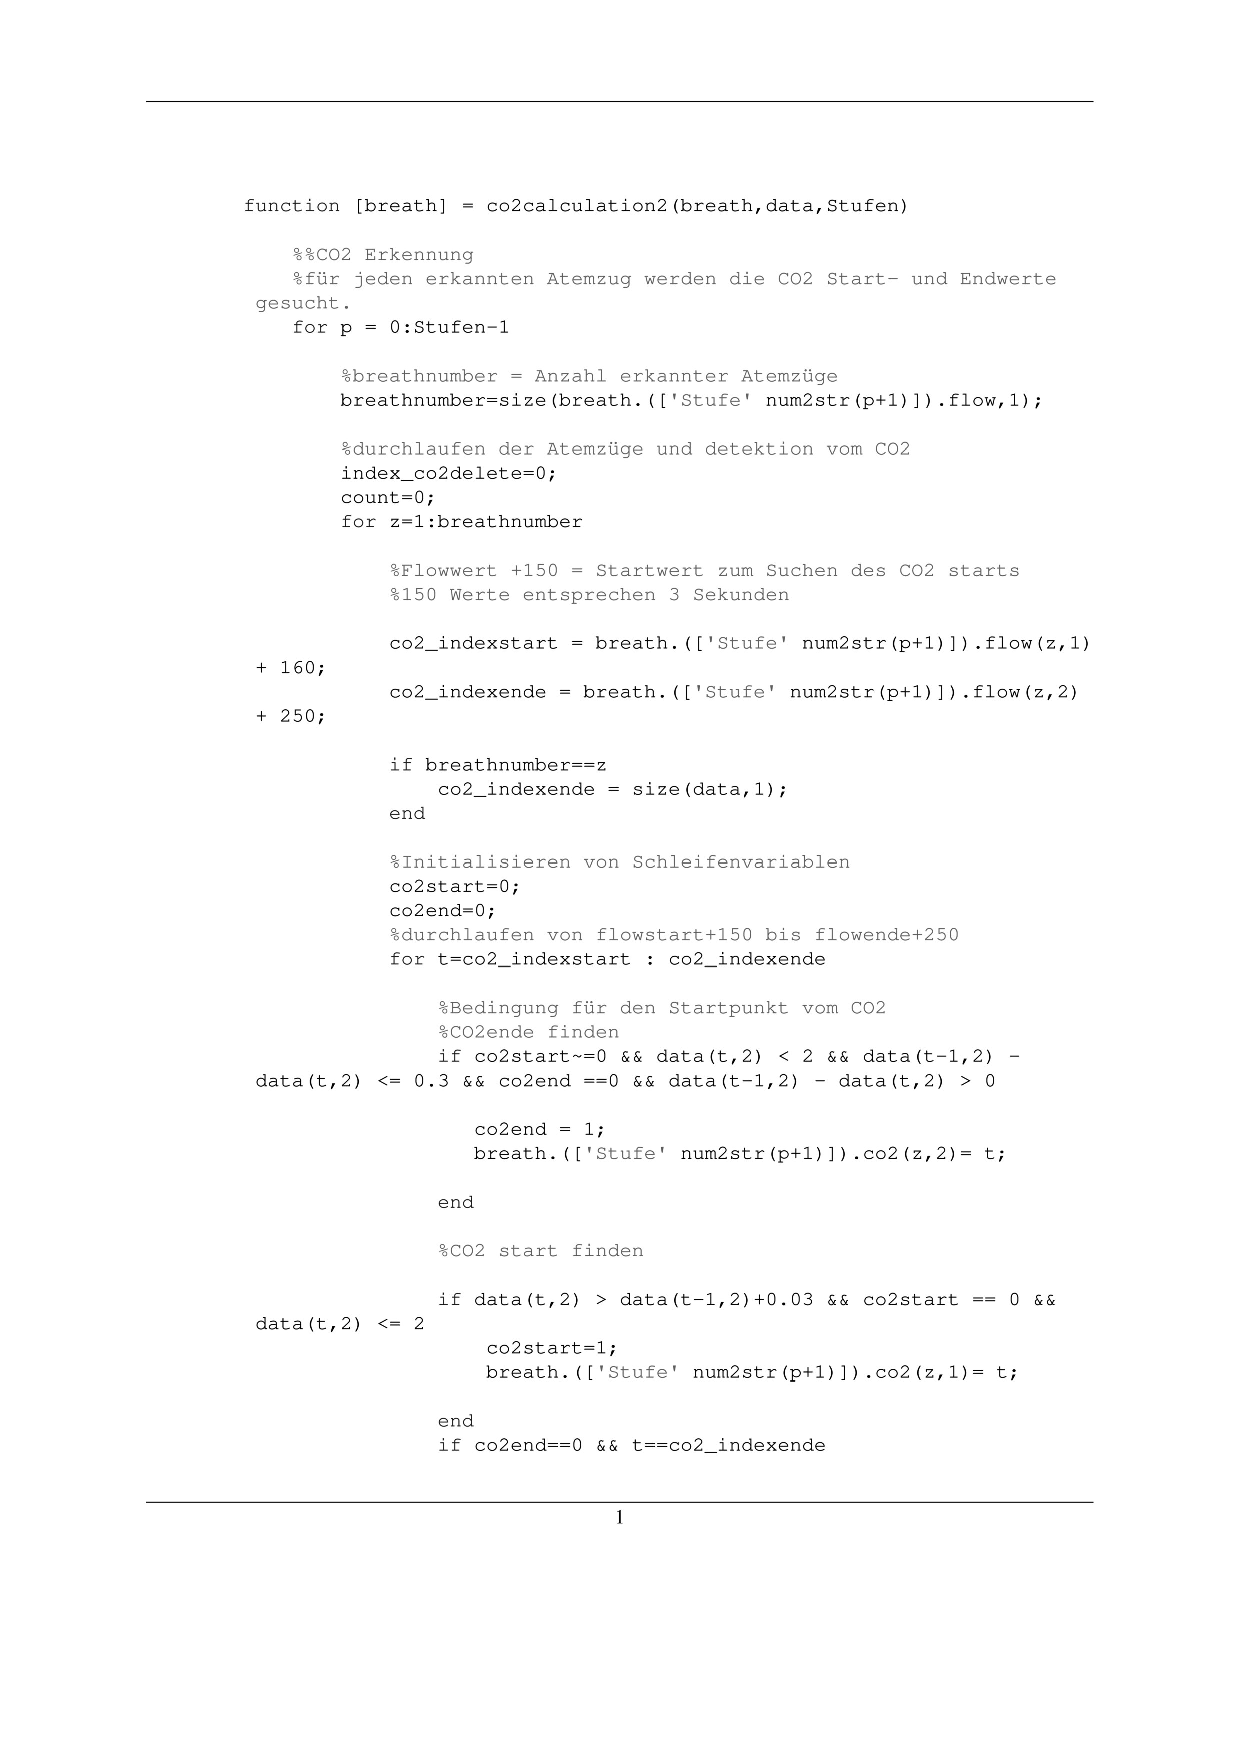
\includepdf[pages=-]{Anhang/co2calculation2.pdf}
%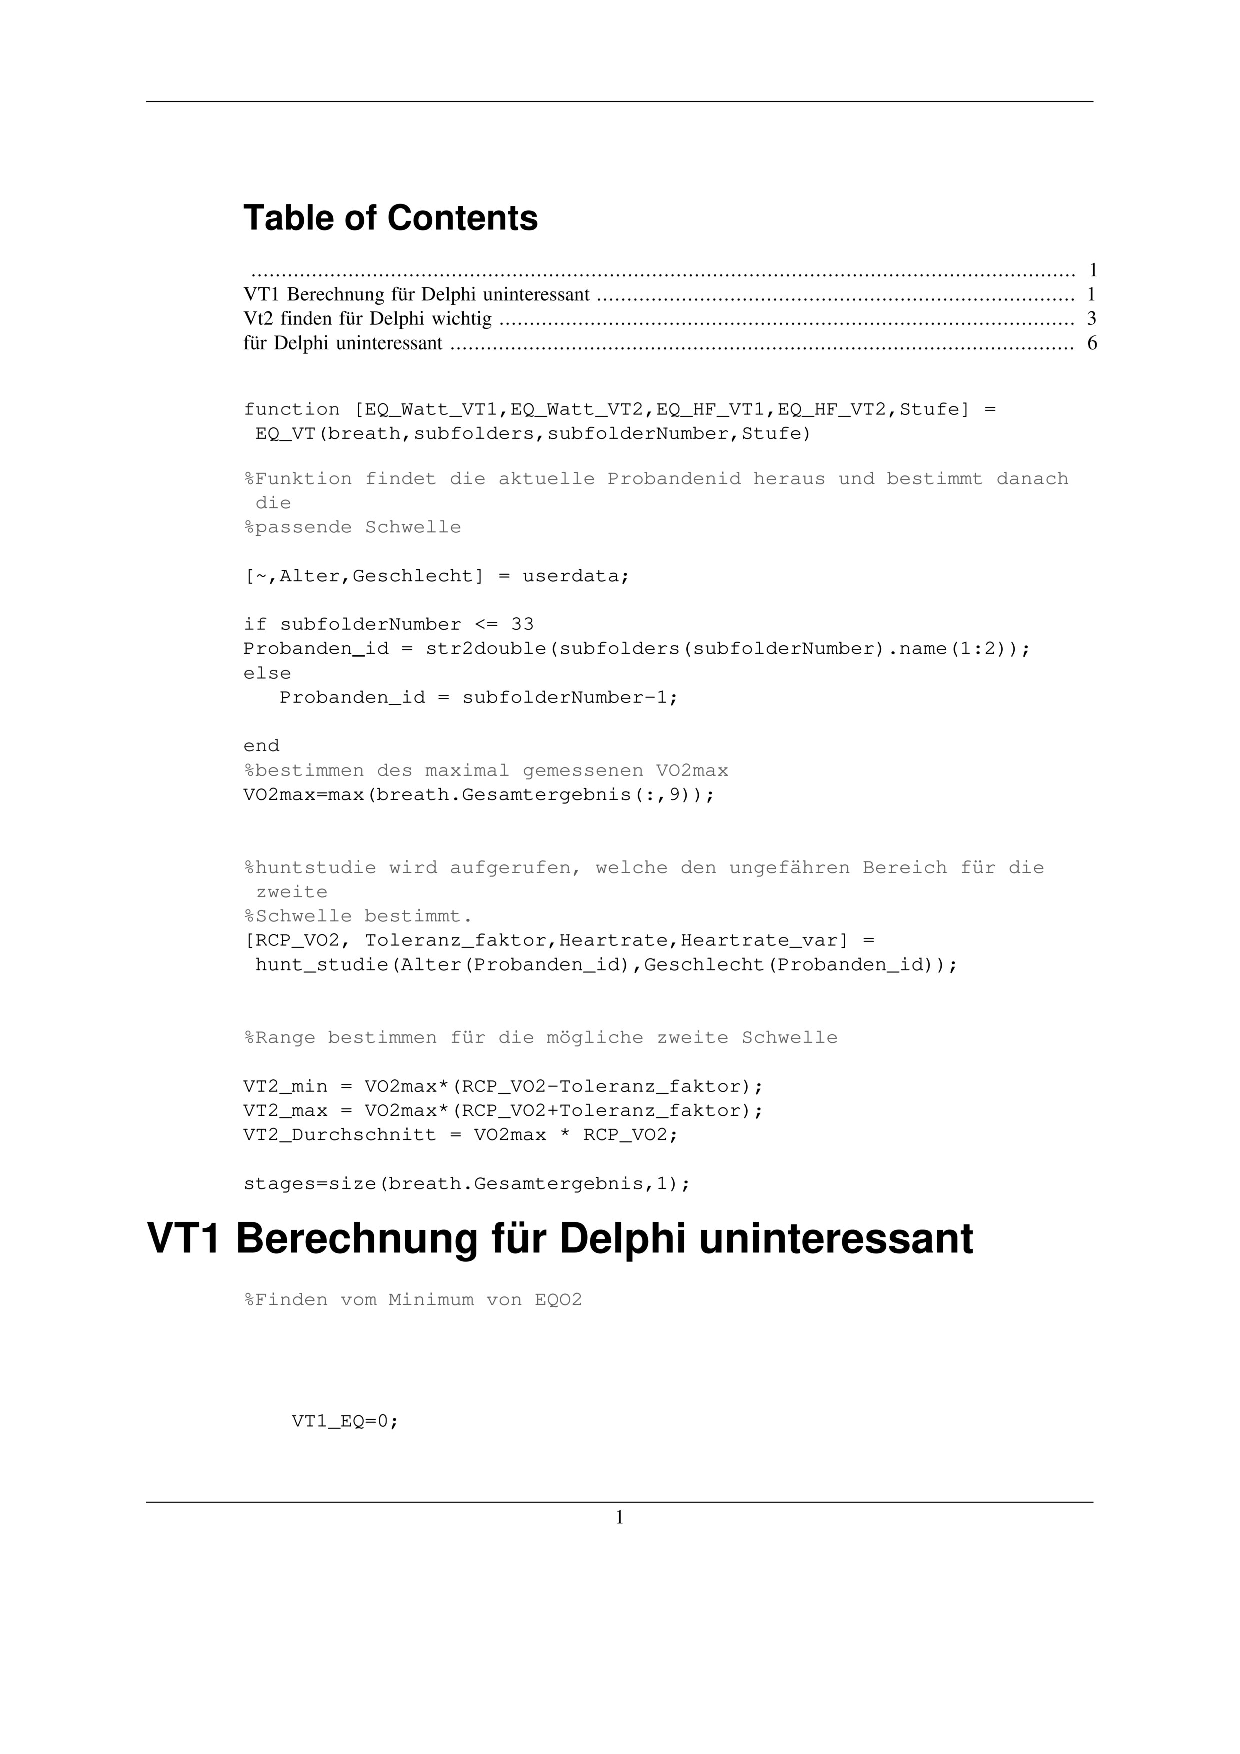
\includepdf{Anhang/EQ_VT.pdf}
	
	\backmatter
%	\subsubsection*{Danksagungen}%\addcontentsline{toc}{chapter}{Danksagungen}

Ich danke meinen Betreuern Prof. Dr. Dipl.-Ing. Ullrich Wenkebach und M. Sc. Lucas Davenport sowie allen hilfsbereiten Kollegen der Firma cardioscan GmbH. Außerdem danke ich meiner Freundin, meiner Familie und meinen engsten Freunden für ihre moralische Unterstützung.


\endinput
	
	
\end{document}



\endinput

